\documentclass[fontsize=12pt,paper=a4,twoside=semi,parskip=half-,headsepline,headinclude]{scrreprt}
% Grundgröße 12pt, zweiseitig
\usepackage[headsepline,automark]{scrlayer-scrpage}
% Seitenköpfe automatisch 
\usepackage[ngerman]{babel}
% Sprachpaket für Deutsch (Umlaute, Trennung,deutsche Überschriften)
\usepackage{blindtext}
% macht nur den Blindtext, den Sie aktuell sehen
\usepackage{lmodern}
% schöne PDF-Schrift
\usepackage{graphicx,hyperref,amssymb}
\hypersetup{pdfborder=0 0 0}
\usepackage{float}
%Graphikeinbindung, Hyperref (alles klickbar, Bookmarks),
%Math. Symbole aus AmsTeX
\usepackage[utf8]{inputenc}
% Umlaute und über Tastatur einzugeben
\usepackage{listings}
\usepackage{xcolor}

\usepackage[table]{xcolor}
\usepackage{colortbl}      % Für Hintergrundfarben
\usepackage{array}         % Für Tabellenanpassungen
\usepackage{booktabs}      % Für \Xhline
\usepackage{tabularx} % Dynamische Anpassung von Tabellenbreiten
\usepackage{makecell}

%CSV
\usepackage{pgfplotstable}
\usepackage{csvsimple}
\usepackage{siunitx}
\sisetup{
	round-mode = places,
	round-precision = 4,
	group-separator = {,},
	group-minimum-digits = 3
}

\newcolumntype{L}[1]{>{\raggedright\arraybackslash}p{#1}}
\newcolumntype{Y}{>{\raggedright\arraybackslash}X}

\setlength{\arrayrulewidth}{0.8pt} % Globale Dicke für alle Linien in der Tabelle

% nette Listing-Formatierung
%\usepackage[backend=bibtex]{biblatex}
\usepackage[sorting=none, style=nature]{biblatex}
\addbibresource{literatur.bib}

% Festlegung Kopf- und Fußzeile     
\defpagestyle{meinstil}{%
{\headmark \hfill}
{\hfill \headmark}
{\hfill \headmark\hfill }
(\textwidth,.4pt)
}{%
(\textwidth,.4pt)
{\pagemark\hfill Philipp Ermer}
{\today \hfill \pagemark}
{\today\hfill\pagemark} 
}
\pagestyle{meinstil} 

\raggedbottom
\renewcommand{\topfraction}{1}
\renewcommand{\bottomfraction}{1}
\newcommand{\code}[1]{\texttt{#1}}

%%%%%%%%%%%%%%%%%%%%%%%%%%%%%%%%%%%%%%%%%%%%%%%%%%%%%%%%%%%%%%%%%%%%%%%%%%

\definecolor{dkgreen}{rgb}{0,0.6,0}
\definecolor{gray}{rgb}{0.5,0.5,0.5}
\definecolor{mauve}{rgb}{0.58,0,0.82}
\definecolor{blue}{rgb}{0,0,1}

% Globale Einstellungen für lstlisting
\lstset{
	frame=topbottom,                  % Nur oben und unten ein Strich (kein Kasten)
	framesep=5pt,                      % Abstand zwischen Rahmen und Text
	rulecolor=\color{gray},            % Rahmenfarbe
	backgroundcolor=\color{white},     % Weißer Hintergrund (kein grauer Hintergrund)
	basicstyle=\ttfamily\small,        % Monospace-Schriftart in kleiner Größe
	captionpos=b,                      % Überschrift unten
	xleftmargin=15pt,                  % Linker Rand
	xrightmargin=15pt,                 % Rechter Rand
	showstringspaces=false,            % Leerzeichen in Strings nicht markieren
	keywordstyle=\bfseries\color{blue}, % Optional: Hervorhebung für Schlüsselwörter (falls notwendig)
	commentstyle=\color{green!50!black}\itshape, % Optional: Stil für Kommentare
	stringstyle=\color{red!80!black},  % Optional: Stil für Strings
	breaklines=true,                   % Automatischer Zeilenumbruch
	breakatwhitespace=true,            % Zeilenumbruch an Leerzeichen
	tabsize=3,                         % Tabulatorgröße
	aboveskip=3mm,                     % Abstand vor dem Listing
	belowskip=3mm,                     % Abstand nach dem Listing
	literate=% Global literate definitions
	{ä}{{\"a}}1
	{ö}{{\"o}}1
	{ü}{{\"u}}1
	{Ä}{{\"A}}1
	{Ö}{{\"O}}1
	{Ü}{{\"U}}1
	{ß}{{\ss}}1
}

\lstdefinelanguage{Java}{
	keywords={abstract, assert, boolean, break, byte, case, catch, char, class, const, continue, default, do, double, else, enum, extends, final, finally, float, for, goto, if, implements, import, instanceof, int, interface, long, native, new, null, package, private, protected, public, return, short, static, strictfp, super, switch, synchronized, this, throw, throws, transient, try, void, volatile, while},
	keywordstyle=\color{blue}\bfseries,
	ndkeywords={@Override, @Deprecated, @SuppressWarnings},
	ndkeywordstyle=\color{gray},
	identifierstyle=\color{black},
	sensitive=true,
	comment=[l]{//},
	morecomment=[s]{/*}{*/},
	commentstyle=\color{dkgreen}\ttfamily,
	stringstyle=\color{mauve}\ttfamily,
	morestring=[b]",
	morestring=[b]',
}

\lstdefinelanguage{Kotlin}{
	keywords={package, import, as, typealias, class, interface, this, super, val, var, fun, for, null, true, false, is, in, throw, return, break, continue, object, if, else, while, do, try, when, companion, override, init, constructor, by, catch, finally, where, enum, sealed, annotation, data, inner, tailrec, operator, inline, infix, external, suspend, lateinit, vararg, reified, dynamic, public, private, protected, internal, out},
	keywordstyle=\color{blue}\bfseries,
	ndkeywords={@file, @property, @field, @get, @set, @receiver, @param, @setparam, @delegate},
	ndkeywordstyle=\color{gray},
	identifierstyle=\color{black},
	sensitive=true,
	comment=[l]{//},
	morecomment=[s]{/*}{*/},
	commentstyle=\color{dkgreen}\ttfamily,
	stringstyle=\color{mauve}\ttfamily,
	morestring=[b]",
	morestring=[b]',
}

\lstdefinelanguage{Go}{
	keywords={break, case, chan, const, continue, default, defer, else, fallthrough, for, func, go, goto, if, import, interface, map, package, range, return, select, struct, switch, type, var},
	keywordstyle=\color{blue}\bfseries,
	ndkeywords={append, cap, close, complex, copy, delete, imag, len, make, new, panic, print, println, real, recover},
	ndkeywordstyle=\color{gray},
	identifierstyle=\color{black},
	sensitive=true,
	comment=[l]{//},
	morecomment=[s]{/*}{*/},
	commentstyle=\color{dkgreen}\ttfamily,
	stringstyle=\color{mauve}\ttfamily,
	morestring=[b]",
	morestring=[b]'}

	\DeclareUnicodeCharacter{03BB}{$\lambda$}
\begin{document}    % hier gehts los
	\renewcommand{\figurename}{Abb.}
	
  \thispagestyle{empty} % Titelseite

\includegraphics[width=0.2\textwidth]{hsh_icons/Wortmarke_WI_schwarz}

   {  ~ \sffamily
  \vfill
  {\Huge\bfseries Leistungsanalyse von Thread-Abstraktionen in verschiedenen Programmiersprachen}
  \bigskip

  {\Large 
  Philipp Ermer \\[2ex]
 Master-Arbeit im Studiengang "`Angewandte Informatik"' 
 \\[5ex]
   \today } 
}
 \vfill
  
  ~ \hfill
  
\includegraphics[height=0.3\paperheight]{hsh_icons/H_WI_Pantone1665} 

\vspace*{-3cm}


\newpage 
\thispagestyle{empty}
\quad 


  \newpage \thispagestyle{empty}
 \begin{tabular}{ll}
{\bfseries\sffamily Autor} &  Philipp Ermer \\ 
            & Matrikelnummer: 1313395 \\
            & philipp.ermer@web.de \\[5ex]
{\bfseries\sffamily Erstprüfer:} & Prof. Dr. Holger Peine \\
          & Abteilung Informatik, Fakultät IV \\
         & Hochschule Hannover \\
        & holger.peine@hs-hannover.de \\[5ex]
{\bfseries\sffamily Zweitprüfer:} &Prof. Dr. Robert Garmann \\
          & Abteilung Informatik, Fakultät IV \\
         & Hochschule Hannover \\
        & robert.garmann@hs-hannover.de
\end{tabular}

\vfill

%%%%%%%%%%%%%%%%%%%%%%%%%%%%%%%%%%%%%%%%%%%%%%%%%%%%%%%%%%%%%%%%%%%%%%%%%%%%%%%
% Die folgende Lizenz kann die weitere Verwertung Ihrer Arbeit vereinfachen.
% Wenn Sie Ihre Arbeit nicht unter dem genannten Lizenzvertrag lizenzieren
% möchten, können Sie diesen Abschnitt entfernen.
% Dies hat keinerlei Einfluss auf die Bewertung Ihrer Arbeit.
Soweit nicht anders gekennzeichnet, ist dieses Werk unter einem
Creative-Commons-Lizenzvertrag Namensnennung 4.0 lizenziert.
Dies gilt nicht für Zitate und Werke, die aufgrund einer anderen Erlaubnis
genutzt werden.
Um die Bedingungen der Lizenz einzusehen, folgen Sie bitte dem Hyperlink:\\
\url{https://creativecommons.org/licenses/by/4.0/deed.de}

\vfill
%%%%%%%%%%%%%%%%%%%%%%%%%%%%%%%%%%%%%%%%%%%%%%%%%%%%%%%%%%%%%%%%%%%%%%%%%%%%%%%

\begin{center} \sffamily\bfseries Selbständigkeitserklärung \end{center}
% fett und zentriert in der minipage

Hiermit erkläre ich, dass ich die eingereichte Master-Arbeit
selbständig und ohne fremde Hilfe verfasst, andere als die von mir angegebenen Quellen
und Hilfsmittel nicht benutzt und die den benutzten Werken wörtlich oder
inhaltlich entnommenen Stellen als solche kenntlich gemacht habe. 
\vspace*{7ex}

Hannover, den \today \hfill Unterschrift


\newpage 
\thispagestyle{empty}
\quad 
\newpage


  \pdfbookmark[0]{Inhalt}{contents}
  \tableofcontents  % Inhaltsverzeichnis

\listoffigures      % Abbildungsverzeichnis

\listoftables       % Tabellenverzeichnis

\chapter{Einführung}

\section{Motivation}

In den letzten Jahren hat die Bedeutung von nebenläufigen Prozessen in der Softwareentwicklung erheblich zugenommen. Mit dem Anstieg der Anforderungen an die Performance und Effizienz von Softwareanwendungen, insbesondere im Bereich von Echtzeit- und Cloud-basierten Systemen, sind robuste und leistungsfähige Nebenläufigkeitskonzepte unerlässlich geworden. Dabei ist es nicht ungewöhnlich, dass mehr Zeit mit der Kommunikation zwischen Systemen verbracht wird, als mit den eigentlichen Berechnungen und das Systeme deshalb mehr warten als arbeiten. Dadurch entsteht die Anforderung an Anwendungen eine hohe Parallelität und Nebenläufigkeit zu gewährleisten. Programmiersprachen wie Java, Kotlin und Go tragen dieser neuen Entwicklung Rechnung und bieten unterschiedliche Ansätze zur Umsetzung von Nebenläufigkeit, die jeweils ihre eigenen Vor- und Nachteile haben. Als Motivation für diese Arbeit dient die aktuelle Veröffentlichung von Virtual Threads in Java im September 2023. Diese diente als Anlass für eine fundierte Bewertung der Performance von aktuellen Thread-Abstraktionen in den ausgewählten Programmiersprachen, da es bislang nur begrenzte vergleichende Analysen, für die Performance dieser Konzepte gibt. Diese Masterarbeit soll ein besseres Verständnis dafür schaffen, welche Technologien sich für spezifische Anwendungsfälle am besten eignen.

\section{Ziel der Arbeit}

Das Ziel dieser Arbeit ist es, eine umfassende Leistungsanalyse der verschiedenen Thread-Abstraktionen in den Programmiersprachen Java, Kotlin und Go durchzuführen. Die Auswahl ist auf diese Sprachen gefallen, da als Ausgangspunkt für diese Arbeit die aktuelle Veröffentlichung von Virtual Threads in Java diente. Als zweite Sprache wurde Kotlin gewählt, da diese ebenfalls in der Java Virtual Machine (JVM) läuft und somit eine direkte Konkurrenz zu Java darstellt. Zuletzt wurde Go als eine weitere zu untersuchende Sprache gewählt, da es sich bei Go um eine Sprache handelt die von Beginn an mit dem Fokus auf Nebenläufigkeit entwickelt wurde und somit als ein guter Vergleichspunkt für Nebenläufigkeit dient. Die zu vergleichenden Nebenläufigkeitskonzepte sind dabei im Detail: Java Threads (Platform Threads), Java Virtual Threads, Kotlin Coroutinen und Go Goroutinen. Diese unterschiedlichen Ansätze sollen hinsichtlich ihrer Effizienz, Skalierbarkeit und Ressourcennutzung verglichen werden.

Um dieses Ziel zu erreichen, werden, im Rahmen dieser Masterarbeit, spezifische Benchmarks konzeptioniert und implementiert , die die Leistung der einzelnen Neben\-läufig\-keits\-konzepte unter verschiedenen Bedingungen messen. Die Ergebnisse dieser Benchmarks sollen Aufschluss darüber geben, welches Nebenläufigkeitskonzepte für bestimmte Anwendungsfälle am besten geeignet sind und welche Vor- und Nachteile die jeweiligen Modelle bieten.

Ein weiteres Ziel dieser Arbeit ist es, praktische Empfehlungen für Entwickler zu erarbeiten, die ihnen helfen sollen, das passende Thread-Abstraktion für ihre spezifischen Anforderungen auszuwählen. Durch die Analyse der Stärken und Schwächen der einzelnen Konzepte soll ein tiefgehendes Verständnis dafür geschaffen werden, wie sich die Wahl einer Thread-Abstraktion auf die Gesamtperformance und die Effizienz einer Anwendung auswirkt.

\section{Verwandte Arbeiten}

Zwar gibt es bereits eine breite Auswahl an Arbeiten die sich mit dem Vergleich von Thread-Abstraktionen in unterschiedlichen Programmiersprachen beschäftigen. Jedoch handelt es sich dabei um Momentaufnahmen, die nur den aktuellen Stand der Technik vergleichen. So können die Ergebnisse, durch die Einführung einer neuen Technologie wie Virtual Threads, schnell überholt sein. Deshalb folgt in diesem Kapitel eine Auswahl an Arbeiten, die am nächsten mit dem Thema dieser Arbeit verwandt sind.

In dem Paper \textbf{Concurrency in Go and Java: Performance Analysis} \cite{Togashi2014} von Naohiro Togashi und Vitaly Klyuev wird die Performance von Nebenläufigkeit in Go und Java verglichen. Dafür werden als Benchmark Matrix-Multiplikationen verwendet. Go erzielt dabei deutlich bessere Ergebnisse als Java, jedoch ist das Paper aus dem Jahr 2014 und deshalb kommen bei Java klassische Threads zum Einsatz, bei Go hingegen Goroutinen. Es wird also interessant sein wie die neueren Virtual Threads im Vergleich zu den Goroutinen abschneiden werden.

In dem Paper \textbf{Comparison of Structured Concurrency Constructs in Java and Kotlin – Virtual Threads and Coroutines} \cite{Modric2022} von D. Beronić, L. Modrić, B. Mihaljević und A. Radovan werden die Nebenläufigkeitskonzepte von Threads und Coroutinen in Kotlin mit Threads und Virtual Thread in Java verglichen. Als Benchmark diente ein von den Autoren implementierter HTTP-Server, jeweils in Java und Kotlin, an welchen Anfragen gesendet werden. Als Ergebnis zeigte sich, dass sowohl Threads in Kotlin und Java, sowie Coroutinen und Virtuel Threads, jeweils dicht bei einander lagen und insgesamt die neuen Technologien deutlich besser als die alten abgeschnitten haben. Da das Paper aus dem Jahr 2022 stammt, konnte nur auf eine Vorabversion von den Virtual Threads zurückgegriffen werden. Es wird also interessant sein, ob sich die Performance von Virtual Threads beim finalen Release noch einmal geändert hat. Außerdem wurde die Performance nur anhand eines Benchmarks verglichen, es wird also ebenfalls interessant sein, wie sich die Performance bei anderen Benchmarks verhält.

Arbeiten die Goroutinen in Go mit Coroutinen in Kotlin vergleichen, konnten nicht gefunden werden, dabei könnte ein Vergleich sehr lohnenswert sein, da sie auf sehr ähnliche Konzepte zurückgreifen. Diese Masterarbeit versucht diese Lücke zu schließen.

\section{Gliederung und Aufbau}

Die vorliegende Arbeit ist in sechs Hauptkapitel gegliedert, die systematisch aufeinander aufbauen, um eine umfassende Untersuchung der Thread-Abstraktionen und ihrer Performance in den ausgewählten Programmiersprachen Java, Kotlin und Go zu ermöglichen.

\subsubsection{Kapitel 2: Thread-Abstraktionen}

Dieses Kapitel bildet die theoretische Grundlage der Arbeit. Es werden die spezifischen Thread-Abstraktionen in den für diese Arbeit ausgewählten Programmiersprachen vorgestellt: Java (Platform Threads und Virtual Threads), Kotlin (Coroutinen) und Go (Goroutinen). Abschließend erfolgt ein theoretischer Vergleich dieser Konzepte, um die Gemeinsamkeiten und Unterschiede zu verdeutlichen, die in den späteren Benchmarks untersucht werden.

\subsubsection{Kapitel 3: Testaufbau}

In diesem Kapitel wird die methodische Herangehensweise dieser Arbeit erläutert. Es beschreibt den Testaufbau, sowie die verwendeten Hard- und Software. Besondere Aufmerksamkeit wird den Performancefaktoren gewidmet, anhand derer die Leistung der Nebenläufigkeitskonzepte in den Benchmarks verglichen wird. Darüber hinaus werden die Werkzeuge zur Datenerhebung vorgestellt und ihre Funktionsweise erläutert. Dieses Kapitel stellt somit die methodische Basis für die Durchführung der Benchmarks dar und sichert die Reproduzierbarkeit der Ergebnisse.

\subsubsection{Kapitel 4: Benchmarks}

In diesem Kapitel werden die durchgeführten Benchmarks im Detail beschrieben. Für jeden Benchmark wird das zugrundeliegende Szenario vorgestellt, die Motivation für den Benchmarkt erläutert und der Aufbau des Benchmarks erklärt. Außerdem wird auf Besonderheiten bei der Implementierung der Benchmarks eingegangen. Die Ergebnisse der einzelnen Tests werden anschließend präsentiert, wobei der Fokus auf der Messung von den Performancefaktoren liegt. Um eine nachvollziehbare Übersicht über die Ergebnisse zu bieten, werden die Daten grafisch aufbereitet.

\subsubsection{Kapitel 5: Auswertung}

Auf Basis der im vorherigen Kapitel präsentierten Daten erfolgt in diesem Kapitel eine Analyse der Benchmark-Ergebnisse. Es wird untersucht, wie die unterschiedlichen Nebenläufigkeitskonzepte der Programmiersprachen die Performance beeinflussen. Besonderes Augenmerk liegt auf der Identifikation von Stärken und Schwächen der jeweiligen Konzepte in verschiedenen Anwendungsszenarien. Abschließend wird ein Vergleich zwischen den Sprachen gezogen, um allgemeine Aussagen zur Eignung der einzelnen Konzepte für bestimmte Einsatzgebiete zu treffen.

\subsubsection{Kapitel 6: Zusammenfassung und Ausblick}

Im abschließenden Kapitel werden die wesentlichen Erkenntnisse der Arbeit zusammengefasst. Es wird ein Überblick über die wichtigsten Resultate und die daraus folgenden Schlüsse gegeben. Außerdem wird es einen Ausblick auf zukünftige Forschungsmöglichkeiten in diesem Bereich gegeben. Dabei wird auf potenzielle Weiterentwicklungen der betrachteten Konzepte sowie auf offene Fragen und Herausforderungen eingegangen.

\chapter{Thread-Abstraktionen}

Im folgenden Kapitel werden die unterschiedlichen Thread-Abstraktionen der verschiedenen Programmiersprachen vorgestellt, welche im Rahmen der Master-Arbeit verglichen wurden. Dabei werden ihre Funktionsweisen, sowie ihre Stärken und Schwächen beleuchtet.

\section{Java: Platform Threads}

Java Threads sind die verbreitetste Art um Nebenläufigkeit in Java-Programmen zu erreichen. Mittlerweile werden Threads auch als Platform Threads bezeichnet, um sie leichter von den neu entwickelten Virtual Threads unterschieden zu können. Der Name leitet sich davon ab, dass es sich bei Platform Threads um sogenannte Wrapper handelt, welche einen Betriebssystem Thread umschließen. Das bedeutet, dass für jeden Platform Thread ein Betriebssystem Thread erstellt wird.

\begin{figure}[h]
	\centering
	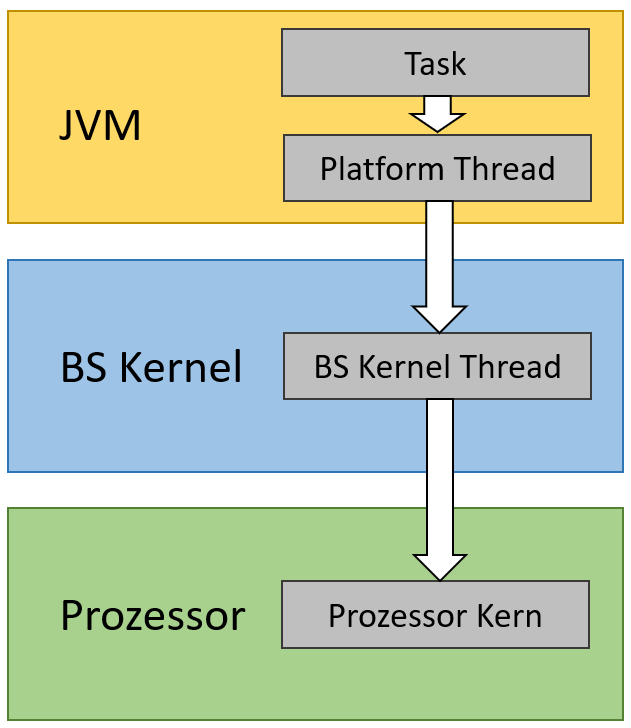
\includegraphics[scale=0.5]{figures/PlatformThreads.png}
	\caption{Aufbau: Java Platform Threads}
	\label{fig:PlatformThreads}
\end{figure}

Dieser Aufbau hat zur Folge, dass Platform Threads schwergewichtig sind. Schwergewichtig meint in diesem Fall, das ein Platform Thread viel Speicher verbraucht($\sim$ 2-3 MB) und es lange dauert ihn zu erstellen($\sim$ 1ms). Platform Threads und die dazugehörigen Betriebssystem Threads sind also ressourcenintensiv und ihre maximale Anzahl ist somit für ein ausführendes System begrenzt. Dies führt dazu, dass die maximale Anzahl der Platform Threads, weit vor anderen Ressourcen, zum limitierenden Faktor wird. 

Eine Lösung um zumindest die Kosten für das Erstellen von neuen Platform Threads zu senken, ist das Verwenden von Thread Pools. Hierbei wird eine Gruppe von Aufgaben einem Pool von Platform Threads zugewiesen. In der Regel übersteigt dabei die Anzahl der Aufgaben die Anzahl an Platform Threads. Dies hat zur Folge, dass einem Platform Thread, nachdem er die ihm zugewiesene Aufgabe abgearbeitet hat, direkt eine neue Aufgabe zugewiesen wird. Das hat den Vorteil, dass nicht mehr für jede Aufgabe ein neuer Platform Thread erstellt werden muss, stattdessen können die gleichen Platform Threads wiederverwendet werden um mehrere Aufgaben hintereinander auszuführen. Damit lassen sich zwar die Kosten für das Erstellen von neuen Platform Threads senken, es lässt sich jedoch nicht die maximale Anzahl an Platform Threads erhöhen.

Ein weiteres Problem ist, dass die Verwaltung der Threads vom Betriebssystem über\-nommen wird und die JRE (Java Runtime Environment) keinen Einfluss darauf nehmen kann. Die Verwaltung der Threads auf Betriebssystemebene muss jedoch sehr allgemein gehalten werden, da sie nicht nur für Java, sondern für alle Programmiersprachen funktionieren muss.

\section{Java: Virtual Threads}

Seit dem JDK 21, welches im September 2023 veröffentlicht wurde, sind Virtual Threads ein fester Bestandteil von Java. Sie wurden ursprünglich im Rahmen des Project Loom als sogenannte Fibers entwickelt. Das Ziel war es die schwergewichtigen Java Threads durch eine leichtgewichtigere Variante zu ersetzen, welche auf die gleiche API (Application Programming Interface) zurückgreift.Dies soll Anwendungsentwicklern den Umstieg von  Platform Threads auf Virtual Threads erleichtern.

Das Ziel von Virtual Threads besteht in der Umgehung der Schwächen von Platform Threads, welche vor allem Anwendungen mit einer großen Anzahl an Threads oder häufig blockierenden Threads sind. Dies gelingt indem eine große Anzahl Virtual Threads auf eine kleine Zahl Betriebssystem Threads verteilt wird. Dadurch werden die Nachteile von Platform Threads umgangen, dass ihre Anzahl stark begrenzt ist und die Verwaltung der Threads auf Betriebssystemebene stattfindet. Stattdessen können Virtual Threads in großer Zahl erstellt werden und die Verwaltung der Threads findet in der JRE statt.

Im Detail sieht dies wie folgt aus:

Es wird eine kleine Anzahl an Platform Threads(Wrapper) erstellt, die ihrerseits einen Betriebssystem Thread umschließen. Diese Platform Threads werden als Carrier Threads bezeichnet, da sie sozusagen den Virtual Thread tragen. Die Anzahl der Carrier Threads entspricht standardmäßig der Anzahl der Prozessorkerne des ausführenden Systems, kann jedoch je nach Anwendungsfall leicht variieren. Die Carrier Threads werden von einem ForkJoinPool verwalten der nach dem FIFO-Prinzip(First In - First Out) und mit work-stealing arbeitet.\cite{Pressler2023a}

Für jede neue Aufgabe (task) im System, die nebenläufig ausgeführt werden kann, wird ein neuer Virtual Thread erstellt. Die Aufgabe bleibt dabei die ganze Zeit im gleichen Virtual Thread. Der Virtual Thread wiederum wird zum Bearbeiten der Aufgabe in einen Carrier Thread eingesetzt (mount). 

\begin{figure}[h]
	\centering
	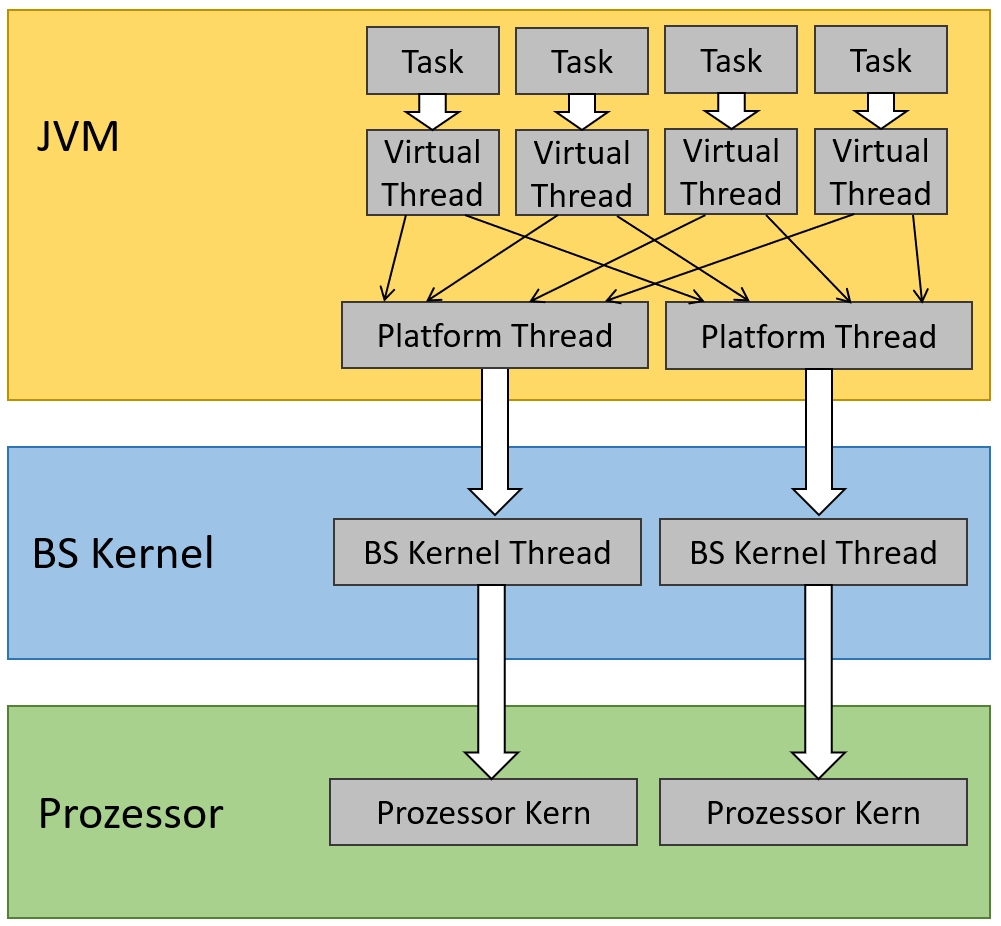
\includegraphics[scale=0.5]{figures/VirtualThreads.png}
	\caption{Aufbau: Java Virtual Threads}
	\label{fig:VirtualThreads}
\end{figure}
%TODO: Grafik überarbeiten Peine: Ungeschickte Grafik: Wirkt so, als ob ein Platform Thread gleichzeitig drei VTs ausführt.

Dort bleibt der Virtual Thread so lange bis die Aufgabe abgeschlossen ist oder der Thread blockiert. Sollte es zu einer Blockade, zum Beispiel durch eine I/O-Operation, kommen, wird der Virtual Thread aus dem Carrier Thread entnommen (unmount) und so lange geparkt, bis er nicht mehr blockiert ist und die Bearbeitung der Aufgabe fortgesetzt werden kann. Der Virtual Thread wir dann wieder in einen freien Carrier Thread eingesetzt, dies kann aber ein andere sein als zu Beginn. Daraus folgt, eine Aufgabe wird ihre gesamte Lebenszeit vom gleichen Virtual Thread ausgeführt, welcher jedoch in unterschiedliche Carrier Threads eingesetzt werden kann. 

Dies stellt eine entschiedene Neuerung gegenüber den Platform Threads dar. War es bisher so, dass ein Platform Thread fest mit einem Betriebssystem Thread verknüpft war, wurde diese Verknüpfung für Virtual Threads aufgehoben. Dies hat den Vorteil, dass ein Virtual Thread einen Carrier Thread und den damit verbundenen Betriebssystems Thread nur dann benutzt, wenn der Virtual Thread Berechnungen auf dem Prozessor ausführt. Ist ein Virtual Thread blockiert macht er platzt auf dem Betriebssystem Thread für einen anderen Virtual Thread. Bei Platform Threads hingegen blockiert nicht nur der Platform Thread sondern auch der zugrunde liegende Betriebssystem Thread. \cite{Bateman2023}

\begin{figure}[h]
	\centering
	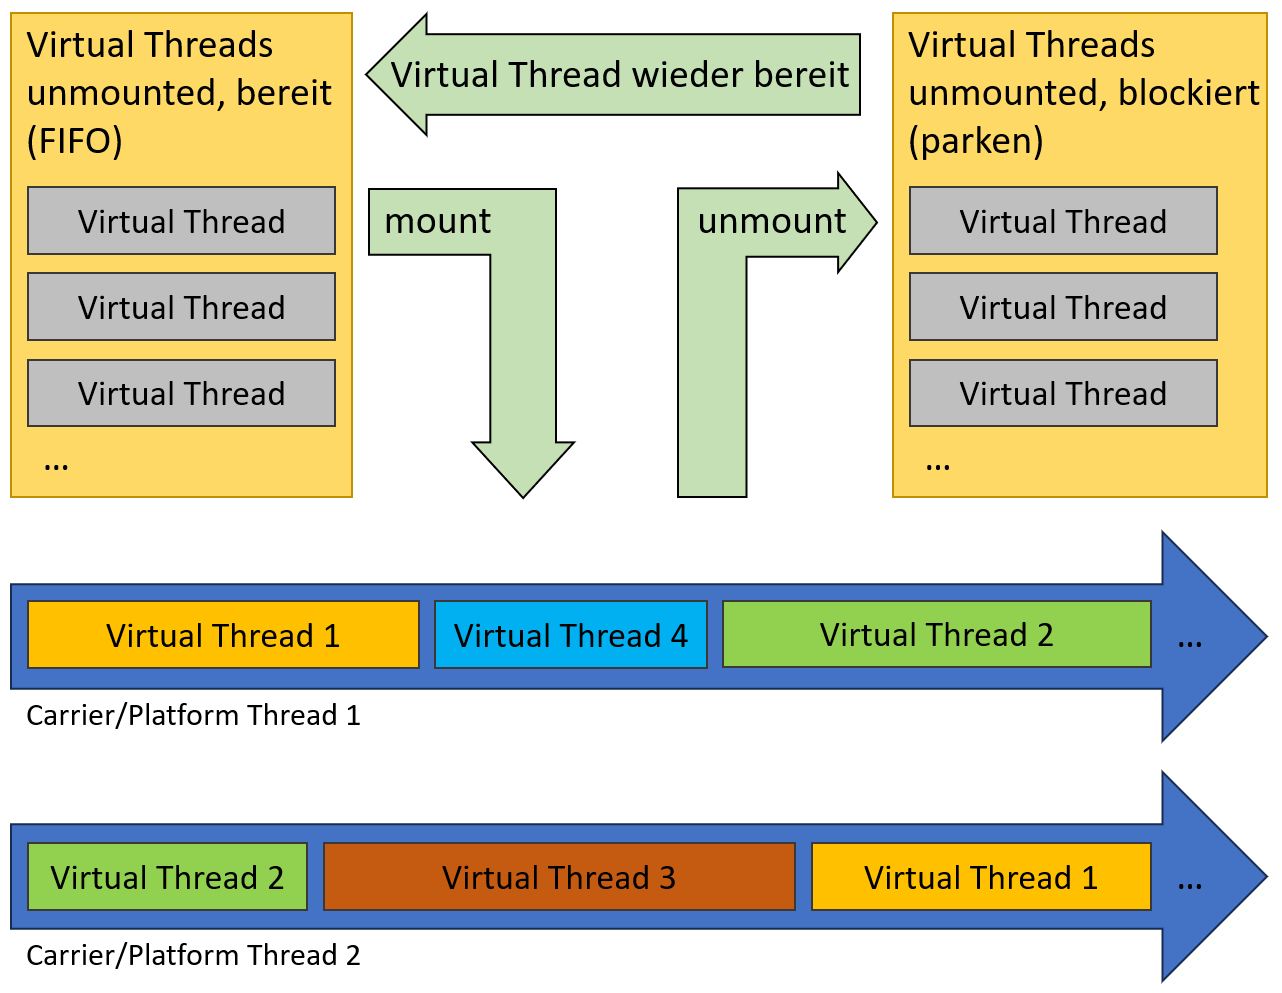
\includegraphics[scale=0.5]{figures/VirtualThreadsAblauf.png}
	\caption{Verwaltung: Java Virtual Threads}
	\label{fig:VirtualThreadsAblauf}
\end{figure}

\subsection{Continuations}

Das beschriebene Starten (mount) und Parken (unmount) von Virtual Threads wird mit Continuations gelöst. Ein Virtual Thread umschließt die ihm übergeben Aufgabe mit einer Continuation. Diese bietet die Methode \code{Continuation.run()} an, um die enthaltene Aufgabe entweder zum ersten Mal zu starten oder sie nach dem Parken fortzusetzen. Letzteres wird auf der Ebene der Continuations als Auftauen (thaw) bezeichnet. Des weiteren gibt es die Methode \code{Continuation.yield()} um eine Aufgabe zu pausieren, wenn sie blockiert. Dies wird im Kontext der Continuations als einfrieren (freeze) bezeichnet. Zuletzt stellen Continuations noch die Methode \code{Continuation.isDone()}(Rückgabewert: boolean) zur Verfügung, um zu überprüfen ob die enthaltene Aufgabe abgeschlossen wurde. Um die Funktionalität der Continuations umzusetzen, musste das gesamte JDK auf Stellen überprüft werden, an denen eine Aufgabe potenziell blockieren kann. An entsprechenden Stellen musste neuer Code hinzugefügt werden, der mit den Continuations kommuniziert, um so eine Aufgabe entweder einzufrieren oder später wieder aufzutauen.\cite{Pressler2023b}

Wenn es um das Blockadeverhalten von Virtual Threads geht gibt es einen Spezialfall, der nach Möglichkeit vermieden sollte, das sogenannte Feststecken (pinning). Dies beschreibt den Fall, wenn die im Virtual Thread enthaltene Aufgabe blockiert und der Virtual Thread nicht aus dem ausführenden Carrier Thread entnommen werden kann. Dies führt dazu, dass nicht nur der Virtual Thread, sondern auch der Carrier Thread blockiert. Dies kann entweder dadurch ausgelöst werden, dass der Thread blockiert während er nativen Code aufruft oder der Thread blockiert, während er Code ausführt der sich in einem Synchronized Block befindet. Synchronized wird verwendet, um den gleichzeitigen Zugriff auf eine Methode oder einen Codeblock zu verhindern, damit nur ein Thread zu einem bestimmten Zeitpunkt Zugriff auf den synchronisierten Code hat. Sollte der Code im Synchronized Block lange blockieren, kann es sinnvoll sein das Synchronized durch ein Reentrant Lock zu ersetzen und dieses freizugeben und dann den Platform-Thread abzugeben (unmount). Die Beschränkung durch Synchronized, soll laut den Virtual Thread Entwicklern in einer zukünftigen Version aufgehoben werden.\cite{Chilano2024} Die Beschränkung durch das Aufrufen von nativen Code wird jedoch bestehen bleiben.\cite{Bateman2024}

\subsection{Thread per request Modell}

Ein typischer Anwendungsfall für Virtual Threads ist eine Server-Anwendung, die Anfragen im Thread per request Modell bearbeitet. Für jede neue Anfrage wird ein neuer Thread erstellt, der diese Anfrage bearbeitet. So können mehrere Anfragen nebenläufig berarbeitet werden. Dies würde bei Platform Threads bedeuten, dass für jede neue Anfrage nicht nur ein neuer Platform Thread, sondern auch ein neuer Betriebssystem Threads erstellt werden muss. Da die Anzahl an Betriebssystem Thread aber für ein System stark limitiert ist, in der Regel auf einige Tausend Stück, ist damit auch die Anzahl der nebenläufig zu bearbeitenden Anfragen limitiert. So werden Platform Threads zum limitierenden Faktor des Systems. Virtual Threads hingegen sind deutlich leichtgewichtiger, da ihre Anzahl nicht an die zur Verfügung stehenden Betriebssystem Threads gebunden ist. Dadurch lässt sich eine große Anzahl von ihnen erstellen, bis zu mehrere Millionen Stück.

Der Vorteil von Virtual Thread gegenüber Platform Threads bei dem Thread per request Modell, lässt sich gut an Little's Gesetz zeigen. Es besagt, dass die sich gleichzeitig in Bearbeitung befindlichen Aufgaben(L) davon abhängig sind, wie hoch der Durchsatz($\lambda$) und die Durchlautzeit (W) sind.\cite{Little1961}

\begin{eqnarray}
	L = \lambda \cdot W \nonumber
\end{eqnarray}

Daraus folgt, dass der Durchsatz sich aus den gleichzeitig in Bearbeitung befindlichen Aufgaben und der Durchlaufzeit ergibt.

\begin{eqnarray}
	\lambda = \frac{L}{W} \nonumber
\end{eqnarray}

Auf das Thread per request Modell angewandt bedeutet das, dass der Durchsatz die pro Sekunde in das System eingehend Anfragen ist. Die Durchlaufzeit wird dadurch beschrieben wie hoch die durchschnittlich Latenz des Systems ist um eine Anfrage zu beantworten. 

Gehen wir also von einem System aus, das 200 Anfragen pro Sekunde verarbeitet, bei einer Latenz von 50ms pro Anfrage. Dafür ist es nötig 10 Anfragen gleichzeitig nebenläufig zu verarbeiten. Soll das System nun auf 2000 Anfragen pro Sekunde, bei gleichbleibender Latenz, skaliert werden, muss das System nun 100  Anfragen gleichzeitig nebenläufig verarbeiten.

Da wir vom Thread per request Modell ausgehen, müssen also im Fall von  Platform Threads 100 von ihnen erstellt werden und damit auch 100 Betriebssystem Threads. Somit ist die Skalierbarkeit auf die maximal zur Verfühgung stehenden Betriebssystem Threads (einige Tausend) begrenzt. Virtual Threads hingegen lassen sich in einer deutlich größeren Anzahl erstellen (mehrere Millionen) und werden so nicht zum limitierenden Faktor wenn es um die Skalierbarkeit des beschriebenen Beispiels geht.

Die Annahme stimmt allerdings nur so lange, wie die nebenläufig bearbeiteten Aufgaben weiterhin mit der gleichen Latenz bearbeitet werden. Dies ist zum Beispiel dann der Fall, wenn eine Aufgabe pausiert wird um auf eine I/O-Operation zu warten. Wenn die einzelne Aufgaben jedoch rechenintensiv sind und möglicherweise niemals pausieren verlieren Virtual Threads ihren Vorteil gegenüber Platform Threads. Virtual Threads können nicht einzelne Aufgaben schneller ausführen als Platform Threads, sondern mehr Aufgaben nebenläufig bearbeiten, falls die Aufgaben manchmal blockieren. 

Damit lässt sich abschließend sagen, dass Virtual Threads den Durchsatz einer Anwendung gegenüber Platform Threads steigern, wenn viele Aufgaben nebenläufig ausgeführt werden und diese Aufgaben manchmal pausieren müssen.

\subsection{Softwareentwicklung mit Virtual Threads}

Eine weitere Zielsetzung von Virtual Threads war es, Softwareentwicklern den Umstieg von Plattform Threads zu Virtual Threads so einfach wie möglich zu gestalten. Deshalb sind Virtual Threads genau wie Plattform Threads eine Instanz der \code{java.lang.Thread} API. So ist es relativ einfach möglich Virtual Threads zu integrieren, ohne die bestehende Codebasis wesentlich zu verändern.

Am folgendem Code-Beispiel wird deutlich, dass lediglich der Aufruf \code{new Thread())} durch \code{Thread.ofVirtual().start()} ersetzt werden muss. Das Starten des Virtuel Threads passiert jetzt direkt beim Aufruf, der restliche Code jedoch unberührt bleibt.

\begin{lstlisting}[language=Java]
	//erstellen eines einzelnen Platform Threads	
	Thread platformThread = new Thread(() -> System.out.println("Platform Thread"));
	platformThread.start();
	platformThread.join();

	//erstellen eines einzelnen Virtual Threads
	Thread virtualThread = Thread.ofVirtual().start(() -> System.out.println("Virtual Thread"));
	virtualThread.join();
\end{lstlisting}

Für Virtual Threads wurde der neue Executor Service \code{Executors.""newVirtualThread""PerTask""Executor()} entwickelt. Für jeden Aufruf von \texttt{ExecutorService.""submit(""Run""nable)} wird ein neuer Virtual Thread erstellt, der die ihm zugewiesene Aufgabe ausführt. Der Rückgabewert des Executor Service ist ein Future, welches das Ergebnis der Aufgabe enthält, sobald der erstellte Virtual Thread ausgeführt wurde. Mit Hilfe von \code{Executors.""newVirtualThread""PerTaskExecutor()} lässt sich ein bestehender Code leicht von Platform Threads auf Virtual Threads umstellen. Oft wird für das Verwalten von Platform Threads ein Thread Pool erstellt und für das Erstellen eines Thread Pools ein Executor Service verwendet. So könnten die Plattform Threads beispielsweise bisher in \code{Executors.newCachedThreadPool()} verwaltet worden sein. Dieser lässt sich nun leicht durch \code{Executors.newVirtualThreadPerTaskExecutor()} ersetzen. Dies wird auch am folgenden Beispiel deutlich:

\begin{lstlisting}[language=Java]
	//mehrere Platform Threads mit Executors.newCachedThreadPool() erstellen
	try (var cachedPool = Executors.newCachedThreadPool()) {
		var future1 = cachedPool.submit(() -> powerFunction(task1.base, task1.exponent));
		var future2 = cachedPool.submit(() -> powerFunction(task2.base, task2.exponent));
		int ptResult1 = future1.get();
		int ptResult2 = future2.get();
	
		System.out.println("Platform Thread Result 1: " + ptResult1);
		System.out.println("Platform Thread Result 2: " + ptResult2);
	} catch (ExecutionException | InterruptedException e) {
		throw new RuntimeException(e);
	}

	//mehrere Virtual Threads mit Executors.newVirtualThreadPerTaskExecutor() erstellen
	try (var executor = Executors.newVirtualThreadPerTaskExecutor()) {
		var future1 = executor.submit(() -> powerFunction(task1.base, task1.exponent));
		var future2 = executor.submit(() -> powerFunction(task2.base, task2.exponent));
		int vtResult1 = future1.get();
		int vtResult2 = future2.get();
	
		System.out.println("Virtual Thread Result 1: " + vtResult1);
		System.out.println("Virtual Thread Result 2: " + vtResult2);
	} catch (ExecutionException | InterruptedException e) {
		throw new RuntimeException(e);
	}
\end{lstlisting}
Der \code{Executors.newVirtualThreadPerTaskExecutor()} erstellt für jede Aufgabe einen neuen Virtual Thread und dient nicht als klassischer Thread Pool, wie der \code{Executors.""newCachedThreadPool()}. Stattdessen wird jede Aufgabe direkt in einem neuen Virtual Thread ausgeführt. Virtual Threads benötigen keinen von der Anwendung explizit verwalteten Thread Pool, da sie von der JVM automatisch auf Plattform-Threads ausgeführt werden. Diese Plattform-Threads werden intern in einem eigenen Thread Pool verwaltet. Der \code{Executors.newVirtualThreadPerTaskExecutor()} nutzt lediglich die gleiche API wie der \code{Executors.newCachedThreadPool()} um den Wechsel von Platform Threads auf Virtual Threads so unkompliziert wie möglich zu gestalten.

Die maximal Anzahl von Virtual Threads ist deutlich größer als die von Platform Threads und die Zeit sie zu erstellen und ihr Speicherverbrauch sind deutlich geringer. Bei der Umstellung auf Virtual Threads werden Platform Threads also nicht direkt durch Virtual Threads ersetzt. Stattdessen werden die Aufgaben durch Virtual Threads ersetzt, beziehungsweise für jede Aufgabe wird ein neuer Virtual Thread erstellt. 

Falls ein Thread Pool bei Platform Threads bisher verwendet wurde um die Anzahl an maximal nebenläufig ausgeführten Aufgaben zu limitieren, sollte dafür bei Virtual Threads stattdessen auf Semaphore zurückgegriffen werden. Auch mit Semaphoren lässt sich die maximale Anzahl gleichzeitiger Zugriffe auf eine Ressource limitieren.

\newpage

\section{Kotlin: Coroutinen}

Coroutinen sind ein zentrales Konzept in Kotlin und werden für die asynchrone Programmierung sowie für nebenläufige Prozesse genutzt. Sie ermöglichen es, komplexe Abläufe einfacher zu schreiben und verständlicher zu gestalten. Im Gegensatz zu herkömmlichen Threads sind Coroutinen jedoch leichtgewichtiger und blockieren keinen Thread während ihrer Ausführung. Dies wird durch die Nutzung eines Thread-Pools ermöglicht, auf dem Coroutinen kooperativ ausgeführt werden. Dieses Kapitel wird die Grundlagen von Coroutinen, deren Implementierung und fortgeschrittene Anwendungsfälle erklären.



\subsection{Motivation}

Bevor es Coroutinen in Kotlin gab, wurde asynchroner Code häufig mit Callbacks umgesetzt. Dabei handelt es sich um ein Programmierkonzept, bei dem einer Funktion als Argument eine andere Funktion übergeben wird, um zu einem späteren Zeitpunkt aufgerufen zu werden. Dies ermöglicht eine flexible und modulare Strukturierung von Programmen, da verschiedene Operationen oder Ereignisse mit spezifischen Reaktionen verknüpft werden können. 

In der Programmierung unterscheidet man zwischen synchroner und asynchroner Ausführung:

Synchrone Ausführung bedeutet, dass der Code in der Reihenfolge ausgeführt wird, in der er geschrieben steht. Das heißt, die Ausführung einer Funktion blockiert den weiteren Ablauf des Programms, bis sie abgeschlossen ist. Ein Beispiel für synchrone Ausführung wäre, wenn wir auf das Ergebnis einer Dateioperation warten und das Programm erst dann fortsetzt, wenn das Ergebnis vorliegt.

Asynchrone Ausführung bedeutet, dass eine Funktion gestartet wird, aber das Programm nicht darauf wartet, dass sie abgeschlossen wird. Stattdessen kann das Programm während der Ausführung dieser Funktion andere Aufgaben fortsetzen, ohne blockiert zu werden. Bei asynchroner Ausführung können Callbacks genutzt werden, um das Ergebnis der Funktion zu verarbeiten, wenn sie abgeschlossen ist.

Callbacks sind besonders nützlich in der asynchronen Programmierung, da Operationen wie das Lesen von Dateien, das Abrufen von Daten über das Netzwerk oder das Warten auf Benutzereingaben ohne Blockieren des Hauptprogramms ausgeführt werden können.

Das folgende Beispiel zeigt, wie asynchrone Operationen mithilfe von Callbacks umgesetzt werden:

\begin{lstlisting}[language=Kotlin]
	import java.io.File
	import kotlin.concurrent.thread
	
	fun readFileAsync(filename: String, callback: (String) -> Unit) {
		thread {
			val content = File(filename).readText()
			callback(content)
		}
	}
	
	fun main() {
		readFileAsync("example.txt") { content ->
			println("File Content: $content")
		}
		println("Read File...")
	}
\end{lstlisting}

In dem gezeigten Beispiel liest die Funktion \texttt{readFileAsync} den Inhalt einer Datei in einem separaten Thread ein und verwendet einen Callback, um das Ergebnis zu verarbeiten. Der Callback wird als Lambda-Ausdruck an \texttt{readFileAsync} übergeben und ausgeführt, nachdem das Einlesen abgeschlossen ist. Der Haupt-Thread wird währenddessen nicht blockiert und kann andere Aufgaben ausführen.

Da es ich bei dem gezeigten Beispiel um eine asynchrone Ausführung handelt kann icht vorhergesehn werden ob erst \texttt{"File Content: [Dateiinhalt]"} oder \texttt{"Read File..."} ausgegeben wird, da die Dateioperation auf separaten Threads ausgeführt werden.

Würde das Starten des Threads in \texttt{readFileAsync} weggelassen, würde es ich um einen synchronen Aufruf handeln. Die Ausgabe wäre dann zuerst \texttt{"File Content: ""[Datei""inhalt]"} und danach \texttt{"Read File..."}, da der Haupt-Thread auf das Ergebnis der Dateioperation warten würde, bevor er fortfährt.

Callbacks sind folglich eine gängige Variante um asynchronen Code zu schrieben, Ein Nachteil jedoch ist die Verwendung vieler verschachtelter Callbacks, welche umgangssprachlich als Callback Hell bezeichnet werden\cite{Leger2021}. Die Callback Hell führt dazu, dass der Code schwer lesbar wird. Daraus resultiert eine erhöhte Komplexität bei der Wartung und dem Debuggen. Die Verschachtelungen machen die Rückverfolgung des Programmflusses kompliziert und  die Fehlerbehandlung wird immer aufwendiger, da sie auf jeder Ebene der Verschachtelungen stattfinden muss.

\begin{lstlisting}[language=Kotlin]
	import kotlin.concurrent.thread
	
	// Simuliert eine asynchrone, zeitaufwändige I/O-Operation (z.B. Datei lesen)
	fun readFileAsync(callback: (String) -> Unit) {
		thread {
			try {
				Thread.sleep(500)
				callback("File Content")
			} catch (e: Exception) {
				callback("Error: ${e.message}")
			}
		}
	}
	
	// Simuliert eine asynchrone, zeitaufwändige Netzwerkoperation, bei der Daten verarbeitet werden (z.B. API-Anfrage)
	fun processData(input: String, callback: (String) -> Unit) {
		thread {
			try {
				Thread.sleep(500)
				callback("$input -> Processed Data")
			} catch (e: Exception) {
				callback("Error: ${e.message}")
			}
		}
	}
	
	// Simuliert das asynchrone, zeitaufwändige Speichern von Daten (z.B. in einer Datenbank oder Datei)
	fun saveData(input: String, callback: (String) -> Unit) {
		thread {
			try {
				Thread.sleep(500)
				callback("$input -> Data Saved")
			} catch (e: Exception) {
				callback("Error: ${e.message}")
			}
		}
	}
	
	fun main() {	
		// Callbacks werden verwendet, um das Ergebnis schrittweise zu erhalten
		readFileAsync { result1 ->
			result1.onSuccess { res1 ->
				processData(res1) { result2 ->
					result2.onSuccess { res2 ->
						saveData(res2) { result3 ->
							result3.onSuccess { res3 ->
								println("Final Result: $res3") // Ausgabe des finalen Ergebnisses 
							}
							// Fehlerbehandlung für saveData
							result3.onFailure { error ->
								println("Error in saveData: ${error.message}") 
							}
						}
					}
					// Fehlerbehandlung für processData
					result2.onFailure { error ->
						println("Error in processData: ${error.message}") 
					}
				}
			}
			// Fehlerbehandlung für readFileAsync
			result1.onFailure { error ->
				println("Error in readFileAsync: ${error.message}") 
			}
		}
		// Zeigt an, dass die asynchronen 	Operationen gestartet wurden
		println("Started operations...") 
	}
\end{lstlisting}
Konsolenausgabe:
\begin{lstlisting}[frame=shadowbox, rulecolor=\color{black}, backgroundcolor=\color{gray!10}]
	Started operations...
	Final Result: File Content -> Processed Data -> Data Saved
\end{lstlisting}

In diesem Beispiel werden drei Operationen asynchron mit Callbacks ausgeführt, die jeweils das Ergebnis der vorausgehenden Operation benötigen. Dies führt zu einer Verschachtelung der Aufrufe in der Main-Funktion. Selbst in diesem einfachen Bespiel wird der Code schon deutlich schwerer lesbar im Vergleich zu einer synchronen Programmierweise, nicht zuletzt auf Grund der ebenfalls verschachtelten Fehlerbehandlung.

Genau an diesem Punkt setzt die Entwicklung von Coroutinen an, welche als Ziel haben die Nachteile der Callback Hell zu umgehen und dabei trotzdem die Vorteile der Callbacks zu behalten\cite{Elizarov2017a}. Ermöglicht werden soll das nebenläufige Ausführen von Aufgaben, ohne das Hauptprogramm zu blockieren, bei weiterhin gut lesbarem Code.


\subsection{suspend-Modifier}
\label{subsec:suspend}

Um die Nachteile der Callback Hell zu umgehen, verfolgen die Coroutinen den Ansatz, dass synchroner Code geschrieben wird, welcher dann asynchron ausgeführt wird. Dafür wurde das Schlüsselwort \texttt{suspend} eingeführt\cite{Akhin2024}. Es wird verwendet um Funktionen als suspendierbar (oder "pausierbar") zu kennzeichnen. Es ermöglicht es einer Funktion, ihre Ausführung zu unterbrechen und später fortzusetzen, ohne dabei den aktuellen Thread zu blockieren (wird im Detail in Abschnitt \ref{subsec:csp} erlätert). Dies ist besonders nützlich für die asynchrone Programmierung, da es den Code lesbarer und einfacher zu handhaben macht im Vergleich zu traditionellen Callback- oder Thread-basierten Lösungen. Außerdem werden mit \texttt{async} Coroutinen gestartet, welche die \texttt{suspend}-Funktionen ausführen. Dadurch kann das Code-Beisipiel aus dem vorausgehenden Abschnitt folgender maßen optimiert werden:

\begin{lstlisting}[language=Kotlin]
	import kotlinx.coroutines.*

	// Simuliert eine asynchrone, zeitaufwändige I/O-Operation (z.B. Datei lesen)
	suspend fun readFileAsync(): String {
		delay(500)
		return "File Content"
	}

	// Simuliert eine asynchrone, zeitaufwändige Netzwerkoperation, bei der Daten verarbeitet werden (z.B. API-Anfrage)
	suspend fun processData(input: String): String {
		delay(500)
		return "$input -> Processed Data"
	}

	// Simuliert das asynchrone, zeitaufwändige Speichern von Daten (z.B. in einer Datenbank oder Datei)
	suspend fun saveData(input: String): String {
		delay(500)
		return "$input -> Data Saved"
	}

	fun main() = runBlocking {
		try {
			// Startet alle Operationen gleichzeitig mit 'async' und wartet auf deren Ergebnisse
			val deferred1 = 
				async { readFileAsync() }
			val deferred2 = 
				async { processData(deferred1.await()) }
			val deferred3 = 
				async { saveData(deferred2.await()) }
		
			// Warten auf die Ergebnisse und Ausgabe des finalen Ergebnisses
			println("Final Result: ${deferred3.await()}")
		} catch (e: Exception) {
			println("Error: ${e.message}")
		}
		println("Started operations...")  // Zeigt an, dass die asynchronen Operationen gestartet wurden
	}
\end{lstlisting}
Konsolenausgabe:
\begin{lstlisting}[frame=shadowbox, rulecolor=\color{black}, backgroundcolor=\color{gray!10}]
	Started operations...
	Final Result: File Content -> Processed Data -> Data Saved
\end{lstlisting}

In dem Beispiel werden jene Funktionen mit dem \texttt{suspend}-Schlüsselwort gekennzeichnet, die als asynchrone Operationen ausgeführt werden sollen. Generell ist bei der Verwendung von \texttt{suspend}-Funktionen zu beachten, dass sie nur von anderen \texttt{suspend}-Funktionen oder Coroutinen ausgeführt werden können. Deshalb werden mit \texttt{async} insgesamt 3 Coroutinen gestartet welche die {suspend}-Funktionen asynchron ausführen. Wie genau Coroutinen gestartet werden wird im nächsten Abschnitt gezeigt.

Durch das Verwenden des suspend-Modifiers ist es möglich, in der Main-Funktion eine synchrone Schreibweise zu verwenden, obwohl der Code asynchron ausgeführt wird ohne Threads zu blockieren. Dadurch haben Coroutinen zwei entscheidene Vorteile gegenüber Callbacks. Ersten ist der Code deutlich besser lesbar, da es weder bei den Funktionsaufrufen noch bei der Fehlerbehandlung zu verschachtelungen kommt und zweitens blockieren keine Threads bei der asynchronen Ausführung der \texttt{suspend}-Funktionen. Damit stellen Coroutinen einen deutlichen Fortschritt gegenüber Callbacks dar. 

\subsection{Coroutinen starten}
\label{subsec:corostarten}

Um in Kotlin eine Coroutine zu starten wird ein Coroutinen-Builder verwendet. Nachfolgend werden  die am häufigsten verwendeten Coroutinen-Builder aufgeführt:

\begin{itemize}
	\item \textbf{launch} ist der am häufigsten verwendete Coroutine-Builder und startet eine neue Coroutine, die kein Ergebnis zurückgibt. Er wird hauptsächlich für asynchron auszuführende Aufgaben verwendet, die nach dem fire-and-forget Prinzip gestartet werden.
	\item \textbf{async} startet ebenfalls eine neue Coroutine, gibt aber sofort ein Deferred-Objekt zurück, das ein zukünftiges Ergebnis repräsentiert. Bei Deferred handelt sich um das Äquivalent eines Promise oder Future in Kotlin. Mit \texttt{await()} ist es möglich auf das Ergebnis zu warten.
	\item \textbf{runBlocking} blockiert den aktuellen Thread, bis der Coroutine-Block abgeschlossen ist. Dies ermöglicht es, asynchronen Code in einer synchronen Umgebung auszuführen. Er wird hauptsächlich in Main-Funktionen und Testfällen verwendet.
	\item \textbf{produce} ist ein spezieller Coroutine-Builder, der einen \texttt{ReceiveChannel} erstellt und Werte in diesen Kanal sendet. Der Kanal wird automatisch geschlossen, wenn die Coroutine beendet wird oder eine Ausnahme auftritt. Der Builder wird hauptsächlich für Producer-Consumer-Muster verwendet.
\end{itemize}


\subsubsection{Coroutinen-Builder}

Das folgende Beispiel zeigt den Aufbau eines Coroutinen-Builders anhand der Funktionssignatur des Builders \texttt{launch}.

\begin{lstlisting}[language=Kotlin]
	fun CoroutineScope.launch(
		context: CoroutineContext = EmptyCoroutineContext,
		start: CoroutineStart = CoroutineStart.DEFAULT,
		block: suspend CoroutineScope.() -> Unit
	): Job
\end{lstlisting}

Die Funktionssignatur besteht aus dem Empfänger-Typ \texttt{CoroutineScope}, Funktionsnamen \texttt{launch}, den Parametern \texttt{context}, \texttt{start}, \texttt{block} und dem Rückgabewert \texttt{Job}.

Der Empfänger-Typ \texttt{CoroutineScope} gibt an, in welchem Scope die Coroutine ausgeführt wird. Builder werden als Erweiterungsfunktionen von Scopes ausgeführt und starten die Coroutine in dem enstprechendem Scope. Durch Scopes lassen sich große Mengen von Coroutinen strukturieren. Dies wird im Kapitel \ref{subsec:coroutinescope} genauer erörtert.

Der Parameter \texttt{context} gibt die Rahmenbedingungen vor, unter denen die Coroutine ausgeführt werden soll. Die einzelnen Bestandteile eines Contextes werden im Kapitel \ref{subsec:coroutinecontext} erklärt.

Der Parameter \texttt{start} gibt an, wann die Coroutine gestartet wird. Dafür kann eine \texttt{CoroutineStart} Enumeration übergeben werden. Der Standardwert ist \texttt{CoroutineStart.""DEFAULT}, was bewirkt, dass die Coroutine sofort gestartet wird.

Im Parameter \texttt{block} wird der von der Coroutine auszuführende Code gespeichert. Wie der Code konkret von der Coroutine ausgeführt wird, wird im Kapitel \ref{subsec:csp} genauer erklärt.

Abschließend hat der Builder als Rückgabewert ein Job-Objekt. Seine Funktionsweise wird im nachfolgendem Kapitel beschrieben.


\subsection{Job}

Ein Job-Objekt in Kotlin repräsentiert eine Coroutine und ihreren Lebenszyklus. Ein Job wird verwendet, um den Status einer Coroutine zu überwachen und zu kontrollieren. Der Coroutinen-Builder \texttt{launch} hat zum Beispiel ein Job-Objekt als Rückgabewert für genau diesen Zweck. Um den Status der Coroutine zu überwachen stehen folgende Eigenschaften zur Verfügung:

\begin{itemize}
	\item \textbf{isActive:} Gibt \texttt{true} zurück, wenn der Job aktiv und nicht abgeschlossen oder abgebrochen ist.
	\item \textbf{isCompleted:} Gibt \texttt{true} zurück, wenn der Job abgeschlossen ist.
	\item \textbf{isCancelled:} Gibt \texttt{true} zurück, wenn der Job abgebrochen wurde.
\end{itemize}

Um eine Coroutine zu kontrollieren stellt ein Job folgende Funktionen zur Verfügung:

\begin{itemize}
	\item \textbf{start():} Startet den Job, falls er noch nicht gestartet wurde.
	\item \textbf{cancel():} Bricht den Job ab. Alle untergeordneten Coroutinen werden ebenfalls abgebrochen.
	\item \textbf{join():} Eine suspend-Funktion, die wartet, bis der Job abgeschlossen ist.
	\item \textbf{invokeOnCompletion(handler: CompletionHandler):} Fügt einen Handler hinzu, der ausgeführt wird, wenn der Job abgeschlossen ist.
\end{itemize}

Auch das Deferred-Objekt ist ein Job-Objekt für Coroutinen die ein Ergebnis liefern. Es wird beispielsweise von dem \texttt{async} Coroutinen-Builder zurückgeben. Es hat neben den oben genannten Eigenschaften und Methoden noch folgende weitere Funktionen, um die Funktionalität eines Futures erfüllen zu können:

\begin{itemize}
	\item \textbf{await():} Eine suspend-Funktion, die auf das Ergebnis der Coroutine wartet und es zurückgibt.
	\item \textbf{getCompleted():} Gibt das Ergebnis zurück, wenn die Coroutine abgeschlossen ist, oder löst eine Ausnahme aus, wenn die Coroutine noch nicht abgeschlossen ist oder mit einem Fehler beendet wurde.
\end{itemize}

\subsection{Dispatcher}

Beim Starten einer Coroutine mittels Coroutinen-Builder kann ein sogenannter Dispatcher für die Coroutine festgelegt werden. Der Dispatcher bestimmt auf welchem Thread oder Thread-Pool die Coroutine ausgeführt wird. In der Regel wird einer der vier folgenden Dispatcher verwendet:

\subsubsection{Dispatchers.Default}

\begin{itemize}
	\item Wird für CPU-intensive Aufgaben verwendet.
	\item Nutzt einen gemeinsamen Pool von Hintergrund-Threads. Die Anzahl der Threads entspricht der Anzahl der CPU-Kerne, mindestens jedoch 2 Threads.
	\item Der Scheduler nutzt eine Work-Stealing-Strategie für eine maximierte CPU-Auslastung.
	\item Ideal für rechenintensive Operationen, die keine sofortige Benutzerinteraktion erfordern.
	\item Ist der Standard Dispatcher in gängigen Buildern wie launch oder asynch.
\end{itemize}


\subsubsection{Dispatchers.IO}

\begin{itemize}
	\item Optimiert für I/O-intensive Aufgaben wie Netzwerk- und Datenbankoperationen oder das Lesen und Schreiben von Dateien.
	\item Nutzt einen Pool von Threads, der für I/O-Operationen konfiguriert ist.  Standardmäßig enthält er 64 Threads, kann aber bei Bedarf erweitert werden.
	\item Der Scheduler nutzt eine FIFO-Warteschlange für die effiziente Bearbeitung von I/O-Operationen.
	\item Hilft, die Haupt-Threads von langwierigen I/O-Operationen zu entlasten.
\end{itemize}

\subsubsection{Dispatchers.Main}

\begin{itemize}
	\item Wird für Aufgaben verwendet, die auf dem Haupt-Thread ausgeführt werden müssen, z.B. UI-Aktualisierungen.
	\item In Android-Anwendungen ist dies der Haupt-Thread, der für die Benutzeroberfläche verantwortlich ist.
\end{itemize}

\subsubsection{Dispatchers.Unconfined}

\begin{itemize}
	\item Führt Coroutinen im aktuellen Thread aus, bis sie suspendiert werden.
	\item Nach der Suspendierung wird die Coroutine in dem Thread fortgesetzt, der die Wiederaufnahme vornimmt.
	\item Wird selten verwendet und ist hauptsächlich für spezielle Anwendungsfälle (z.B. Testing) gedacht.
\end{itemize}

Die Vorteile des Dispatcher-Ansatzes sind dabei leicht ersichtlich. Mit Hilfe der Dispatcher findet eine Abstrahierung der Thread-Verwaltung statt und es wird Komplexität reduziert. Ein Anwender muss nur noch einen Dispatcher wählen der für die zugewiesene Aufgabe optimiert wurde. Außerdem wird der Code besser lesbar, da sich einem Außenstehenden sofort erschließt, für was für eine Sorte von Aufgabe die Coroutine erstellt wurde. Die Herausforderung für den Anwender ist dabei die Wahl des passenden Dispatchers, da diese für bestimmte Anwendungsfälle optimiert wurden. Außerdem sollte von häufigen Kontextwechseln während der Laufzeit einer Coroutine abgesehen werden, da dies jedes Mal zu einem kleinen  Performance-Overhead führt.

Die Zuweisung eines Dispatchers während des Startens einer Coroutine mit dem Builder \texttt{launch} sieht folgendermaßen aus:

\begin{lstlisting}[language=Kotlin]
	launch(Dispatchers.Default) {
		// CPU-intensive Aufgabe
	}
\end{lstlisting}

\subsection{Coroutinen-Context}
\label{subsec:coroutinecontext}

Das Code-Beispiel aus dem vorangegangenen Kapitel für die Zuweisung eines Dispatchers ist etwas verkürzt, denn ein Coroutinen-Builder benötigt eigentlich einen Coroutinen-Context. Ein Coroutinen-Context wiederum setzt sich aus einem Job, einem Dispatcher und einem Coroutinen-Namen zusammen. Diese Elemente geben die Rahmenbedingungen vor, unter denen eine Coroutine ausgeführt werden soll. Möchte man alle drei Elemente selber festlegen sähe dies wie folgt aus:

\begin{lstlisting}[language=Kotlin]
	import kotlinx.coroutines.*

	fun main() = runBlocking {
		val customContext = Job() + Dispatchers.Default + CoroutineName("MyCoroutine")
	
		launch(customContext) {
			// CPU-intensive Aufgabe
		}
	}
\end{lstlisting}

Das Pluszeichen (+) wird verwendet, um die einzelnen Elemente des Coroutinen-Contexts zu kombinieren, wobei jeder Aufruf des Pluszeichen-Operators einen neuen Context erstellt, der die Eigenschaften der kombinierten Elemente enthält.

Werden beim Erstellen eines Coroutinen-Contextes nicht alle Elemente festgelegt, wird für die weiteren Elemente auf ihre Standardwerte zurückgegriffen. Der Coroutinen-Name ist standardmäßig \texttt{null}, da er nur aus Debugging-Gründen benötigt wird. Der Standard-Dispatcher ist \texttt{Dispatchers.Default}. Wenn kein Job explizit übergeben wird, wird von dem Builder ein neuer Job erstellt. Dies hat Auswirkungen auf die Coroutinen Hierarchie, auf die im Nachfolgenden genauer eingegangen wird.

\subsection{Coroutinen-Scope}
\label{subsec:coroutinescope}

Wie bereits im Abschnitt zu Coroutinen-Buildern erwähnt, sind Builder als  Erweiterungsfunktionen von Coroutinen-Scopes definiert. Das hat zur Folge, dass jede Coroutine in einem Scope ausgeführt wird. Jeder Coroutinen-Scope besitzt einen Context. Dieser kann entweder dem als Scope Übergabeparameter übergeben oder mittels Builder festgelegt werden. Mithilfe von Scopes lassen sich Coroutinen strukturieren, so entsteht eine Hierarchie durch Vererbung. Im Ergebnis lassen sich die Lebenszyklen von Coroutinen leichter kontrollieren und es ist einfacher Coroutinen zu beenden. Der folgende Code ist ein Beispiel für Vererbung:

\begin{lstlisting}[language=Kotlin]
	import kotlinx.coroutines.*

	fun main() = runBlocking {
	
    	val customScope = CoroutineScope(Job() + Dispatchers.Default)

		val parentJob = customScope.launch {
			println("Parent coroutine started")
			
			// Starten von Kind-Coroutinen, die den Eltern-Job erben
			val childJob1 = launch {
				delay(1000)
				println("Child coroutine 1 completed")
			}
		
			val childJob2 = launch {
				delay(2000)
				println("Child coroutine 2 completed")
			}
		
			// Warten auf den Abschluss aller Kind-Coroutinen
			childJob1.join()
			childJob2.join()
			println("Parent coroutine completed")
		}
	
		parentJob.join()
	}
\end{lstlisting}

Zuerst wird der Coroutinen-Scope \texttt{customScope} erstellt, mit einem neuen Job und dem \texttt{Dispatchers.Default}. Dieser Scope definiert die Umgebung, in der alle Coroutinen ausgeführt werden, die innerhalb dieses Scopes gestartet werden. Dann wird die Coroutine \texttt{parentJob} im \texttt{customScope} gestartet. Innerhalb der Eltern-Coroutine werden zwei weitere Coroutinen (\texttt{childJob1} und \texttt{childJob2}) gestartet. Diese Kind-Coroutinen erben den Job und den Dispatcher der Eltern-Coroutine, außerdem werden sie im gleichem Scope ausgeführt. Da sie den gleichen Job erben, werden sie als Kinder der Eltern-Coroutine betrachtet. Bei der Vererbung von Jobs ist anzumerken, dass der Builder dennoch ein neues Job Element für die Kind-Coroutine erstellt, der neue Job ist jedoch ein Kind des Eltern-Jobs. Daraus folgt, dass wenn der Eltern Job abgebrochen wird, werden auch alle seine Kinder-Jobs abgebrochen. Das gleiche gilt für den Scope.  Sollte dieser abgebrochen werden, werden alle Coroutinen, die in ihm gestartet wurden, ebenfalls abgebrochen. Möchte man eine Coroutine zwar innerhalb einer anderen Coroutine starten, sie aber unabhängig von ihr laufen lassen, ist dies auch möglich, indem man sie explizit innerhalb eines eigenen Scopes startet.

Außerdem gibt es bereits vordefinierte Scopes für spezifische Anwendungsfälle. Die drei häufigsten sind: \texttt{lifecycleScope}, \texttt{viewModelScope} und \texttt{GlobalScope}.

\subsubsection{lifecycleScope}

Der \texttt{lifecycleScope} kommt in der Android-Entwicklung zum Einsatz. Dabei ist der Scope mit dem Lebenszyklus einer Komponente (z.B. Activity oder Fragment) verknüpft. Dies stellt sicher, dass Coroutinen, die im \texttt{lifecycleScope} gestartet werden, automatisch abgebrochen werden, wenn die Komponente zerstört wird. Somit werden keine Ressourcen verschwendet, wenn die Komponente nicht mehr aktiv ist.

\subsubsection{viewModelScope}

Der \texttt{viewModelScope} wurde speziell für ViewModels in Android entwickelt. Coroutinen, die in \texttt{viewModelScope} gestartet werden, werden automatisch abgebrochen, wenn das ViewModel gelöscht wird. Dies ist nützlich für Aufgaben, die nur ausgeführt werden sollen, solange das ViewModel aktiv ist, wie z.B. das Laden von Daten einer Benutzeroberfläche.

\subsubsection{GlobalScope}

Zuletzt gibt es noch den \texttt{GlobalScope}. Dieser wird verwendet, um Top-Level-Coroutinen zu starten, die während der gesamten Lebensdauer der Anwendung laufen sollen und nicht vorzeitig abgebrochen werden. \texttt{GlobalScope} ist als "delicate API" (heikle API) markiert, da er leicht zu Ressourcen- oder Speicherlecks führen kann, wenn er nicht richtig verwendet wird. Das rührt daher, dass Coroutinen, die im \texttt{GlobalScope} erstellt werden, außerhalb der Hierarchie der anderen Scopes laufen und so nicht automatisch abgebrochen werden.

\subsection{Cancellation}

Es kann dazu kommen, dass eine Coroutine vorzeitig abgebrochen werden soll. Der Abbruch wird als Cancellation bezeichnetet. Eine Cancellation kann viele Ursachen haben, zum Beispiel wurde die Coroutine direkt über die Methode \texttt{cancel()} abgebrochen oder es wurde die Eltern-Coroutine abgebrochen. Das gleiche gilt wenn der Scope, in dem die Coroutine läuft, abgebrochen wurde oder in der Coroutine eine unbehandelte Ausnahme auftritt.

Kommt es in einer Coroutine zu einer Cancellation, wird auf das Konzept der cooperative Cancellation\cite{Cancellation2024} zurückgegriffen. Das bedeutet eine Coroutine muss an erwartbaren Punkten abbrechbar sein. Im Detail heißt das, dass eine Coroutine in regelmäßigen Abständen selbständig überprüfen muss ob sie noch aktiv ist oder abgebrochen wurde. Dies geschieht zum Beispiel indem in der Coroutine der Zustand von \texttt{isActive} überprüft wird oder die Methode \texttt{ensureActive()} aufgerufen wird.

\begin{lstlisting}[language=Kotlin]
	//nicht abbrechbare Coroutine
	launch {
		while (true) {
			//do something
		}
	}

	//abbrechbare Coroutine
	launch {
		while (this.isActive) {
			//do something
		}
	}
\end{lstlisting}

Alternativ kann auch jede suspend-Funktion aus der kotlinx-Bibliothek verwendet werden, zum Beispiel \texttt{delay()} oder \texttt{yield()}. Alle suspend-Funktion aus der kotlinx-""Bibliothek sind abbrechbar (cancelable) und  durch ihre Verwendung wird auch die aufrufende Coroutine abbrechbar. Letztendlich liegt es jedoch in der Verantwortung der entwickelnden Person die Coroutine so zu gestalten, dass sie cooperative cancelable ist.

\subsection{Continuations}

Continuations sind in Kotlin ein zentraler Bestandteil des Coroutinenen-Konzepts. Continuations repräsentieren den verbleibenden Berechnungsweg ab einem bestimmten Punkt innerhalb einer Coroutine. Eine Continuation ist im Wesentlichen ein Objekt, das den Zustand einer Coroutine zu einem bestimmten Zeitpunkt speichert und es ermöglicht, die Coroutine von diesem Punkt aus fortzusetzen. Sie erfasst, wo die Coroutine ihre Ausführung fortsetzen soll und welche Daten sie dabei mitnehmen muss.

Der Ablauf sieht dafür wie folgt aus. Eine Coroutine führt eine suspend-Funktion aus. Dabei kommt es zu der Situation, dass die suspend-Funktion blockiert. Daraufhin wird die ausführende Coroutine von der suspend-Funktion suspendiert. Der Zustand der Coroutine wird in einer Continuation gespeichert, einschließlich ihrer Position im Code als auch aller lokalen Variablen. Das Suspendieren der Coroutine hat den Vorteil, dass der Thread, der die Coroutine ausführt, nicht blockiert wird und wieder frei ist, um in der Zwischenzeit andere Coroutinen auszuführen. Wenn die suspend-Funktion nicht mehr blockiert ist, kann die Ausführung der Coroutine wieder fortgesetzt werden. Dazu wird das Continuation-Objekt verwendet, mit dessen Hilfe die Coroutine wieder in den Zustand versetzt werden kann, den sie vor der Suspendierung hatte.

Das Continuation Interface sieht dabei folgendermaßen aus:

\begin{lstlisting}[language=Kotlin]
	interface Continuation<in T> {
		val context: CoroutineContext
		fun resumeWith(result: Result<T>)
	}
\end{lstlisting}

\begin{itemize}
	\item \textbf{context:} enthält den Coroutine-Kontext, der ausführenden Coroutine und stellt sicher, dass sie bei Wiederaufnahme im selben Context ausgeführt wird.
	\item \textbf{resumeWith(result: Result$<$T$>$):} ist eine Funktion, um die Coroutine mit einem Ergebnis fortzusetzen. Der Result-Typ kann entweder ein erfolgreiches Ergebnis oder eine Ausnahme enthalten.
\end{itemize}

Außerdem gibt es die beiden Erweiterungsfunktionen \texttt{resume} und \texttt{resumWithException}, welche anstelle von \texttt{resumeWith} verwendet werden können. Die Funktion \texttt{resume} wird eingesetzt um eine Coroutine mit einem erfolgreichen Ergebnis fortzusetzen, die Funktion \texttt{resumWithException} hingegen, wenn es zu einer Ausnahme kam.


\subsection{countinuation-passing style}
\label{subsec:csp}

Für die Verwendung von Continuations in Coroutinen wird auf den countinuation-passing style\cite{sus75} zurückgegriffen. Der zuvor in Kotlin synchron geschriebene Code wird während der Kompilierung in Bytecode in den countinuation-passing style umgewandelt\cite{Elizarov2017b}. Betrachten wir dafür folgenden Beispiel-Code:

\begin{lstlisting}[language=Kotlin]
	import kotlinx.coroutines.*

	fun main() = runBlocking {
		val localVar1 = "Hello"
		val result1 = firstOperation(localVar1)
	
		val localVar2 = 3.14
		val result2 = secondOperation(result1, localVar2)
	
		println("Final Result: $result2")
	}

	suspend fun firstOperation(localVar1: String): String {
		// Hier würde eine asynchrone Operation ausgeführt werden
		return "Result1: $localVar1"
	}

	suspend fun secondOperation(input: String, localVar2: Double): String {
		// Hier würde eine asynchrone Operation ausgeführt werden
		return "$input - Result2: $localVar2"
	}
\end{lstlisting}
Konsolenausgabe:
\begin{lstlisting}[frame=shadowbox, rulecolor=\color{black}, backgroundcolor=\color{gray!10}]
	Final Result: Result1: Hello - Result2: 3.14
\end{lstlisting}

In dem Beispiel wird die \texttt{main}-Funktion mit \texttt{runBlocking} in einer Coroutine ausgeführt. Innerhalb dieser Coroutine werden zwei \texttt{suspend}-Funktionen (\texttt{firstOperation} und \texttt{secondOperation}) nacheinander ausgeführt. Dabei werden zwei lokale Variablen (\texttt{localVar1}, \texttt{localVar2}) erstellt, die als Eingaben für die Funktionen dienen. Obwohl \texttt{suspend}-Funktionen in Kotlin asynchrone Operationen ermöglichen, enthalten sie in diesem Beispiel nur synchrone Logik. Zuletzt gibt die \texttt{main}-Funktion das finale Ergebnis auf der Konsole aus. Durch den Einsatz von \texttt{runBlocking} wird sichergestellt, dass die Coroutine vollständig ausgeführt wird, bevor das Programm endet.

Das nachfolgende Beispiel zeigt in vereinfachter Form, wie der Code nach der Kompilierung in Bytecode aussehen würde. Zum besseren Verständnis wird er in pseudo-Kotlin dargestellt:

\begin{lstlisting}[language=Kotlin]
	fun block(cont: Continuation<Any?>) {
		val sm = cont as? ThisSM ?: object : ThisSM {
			var label = 0
			var localVar1: String = ""
			var result1: String = ""
			var localVar2: Double = 0.0
			var stateResult: Any? = null
		
			override fun resume(value: Any?) {
				this.stateResult = value
				block(this)
			}
		}
	
		when (sm.label) {
			0 -> {
				sm.label = 1
				sm.localVar1 = "Hello"
				val stateResult = firstOperation(sm.localVar1, sm)
				if (stateResult == COROUTINE_SUSPENDED) return COROUTINE_SUSPENDED
			}
			1 -> {
				sm.label = 2
				sm.result1 = sm.stateResult as String
				sm.localVar2 = 3.14
				val stateResult = secondOperation(sm.result1, sm.localVar2, sm)
				if (stateResult == COROUTINE_SUSPENDED) return COROUTINE_SUSPENDED
			}
			2 -> {
				sm.label = -1
				val result2 = sm.stateResult as String
				println("Final Result: $result2")
				return Unit
			}
		}
		return Unit
	}

	fun firstOperation(localVar1: String, continuation: Continuation<String>): Any? {
		return suspendCoroutine { cont ->
			// Hier würde normalerweise eine asynchrone Operation stattfinden
			// Für dieses Beispiel führen wir sie sofort aus
			cont.resume("Result1: $localVar1")
		}
		// Hier würde implizit COROUTINE_SUSPENDED zurückgegeben, wenn die Coroutine blockieren würde
	}

	fun secondOperation(input: String, localVar2: Double, continuation: Continuation<String>): Any? {
		return suspendCoroutine { cont ->
			// Hier würde normalerweise eine asynchrone Operation stattfinden
			// Für dieses Beispiel führen wir sie sofort aus
			cont.resume("$input - Result2: $localVar2")
		}
		// Hier würde implizit COROUTINE_SUSPENDED zurückgegeben, wenn die Coroutine blockieren würde
	}
\end{lstlisting}

Die Funktion \texttt{block} repräsentiert den Code, der innerhalb der Coroutine ausgeführt werden soll. Als Übergabeparameter besitzt die Funktion eine Continuation.

\subsubsection{State Machine}

Als erstes wird die State Machine \texttt{sm} erstellt. Sie ist eine Continuation und repräsentiert den aktuellen Zustand der Coroutine\cite{Elizarov2021}. Wenn der Übergabeparameter \texttt{cont} nicht \texttt{null} ist, wird dieser als State Machine verwendet. Ansonsten wird eine neue Continuation erstellt. Beim ersten Aufrufen der Funktion \texttt{block} ist der Übergabeparameter \texttt{cont} noch \texttt{null} und deshalb wird eine neue Continuation erstellt und als State Machine festgelegt. Um den aktuellen Zustand der Coroutine durchgehend abzubilden müssen zuerst einige Variablen definiert werden.  Die Variable \texttt{lable} gibt an in welchem Zustand sich die State Machine befindet. Außerdem werden die lokalen Variablen \texttt{localVar1}, \texttt{result1}, \texttt{localVar2} initialisiert, da sie in der ebenfalls ursprünglichen \texttt{main}-Funktion vorkamen und ihr Inhalt, deshalb gespeichert werden muss. Zuletzt wird in der Funktion \texttt{resume} festgelegt, was passieren soll, wenn eine suspendierende Operation abgeschlossen ist. In diesem Fall wird das Ergebnis der Operation in \texttt{stateResult} gespeichert und die Funktion \texttt{block} aufgerufen, welcher die Continuation selbst übergeben werden. An dieser Stelle wird schon deutlich, was sich hinter dem countinuation-passing style verbirgt, nämlich eine Form von rekursiven Aufrufen die nicht allzu weit von Callbacks entfernt sind.

\subsubsection{when-Statement}

Nachdem die State Machine erstellt wurde folgt ein \texttt{when}-Statement. Er beinhaltet, in einer modifizierten Weise, den eigentlichen Code aus der ursprünglichen \texttt{main}-Funktion. Der Code wurde dabei auf mehrere Zustände aufgeteilt. Die Unterteilungen fanden jeweils an so genannten suspension-Punkten statt. Dies sind Stellen, an denen der Code potenziell blockieren könnte. In der Regel sind dies Aufrufe von \texttt{suspend}-Funktionen, so auch in diesem Fall. Die Variable \texttt{lable} der State Machine gibt dabei an, welcher der Zustände des \texttt{when}-Blocks ausgeführt werden soll. Zu Beginn hat \texttt{lable} den Wert 0, dementsprechend wird zuerst der Zustand 0 ausgeführt. 

\subsubsection{Zustand 0}

Als erstes in diesem Abschnitt wird \texttt{sm.lable} auf 1 gesetzt. Das bedeutet in der State Machine wird vermerkt, dass beim erneuten Aufrufen von \texttt{block} der Code in Zustand 1 ausgeführt werden soll. Danach wird der eigentlichen Code aus der ursprünglichen \texttt{main}-Funktion ausgeführt. Die lokale Variable \texttt{sm.localVar1} erhält den Wert \texttt{Hello}. Sie ist Teil der State Machine, deshalb bleibt ihr Inhalt über alle Zustände hinweg gespeichert. Als nächstes wird die Funktion \texttt{firstOperation} aufgerufen. Bei dieser handelt es sich um eine \texttt{suspend}-Funktion. Deshalb ist sie ein potenzieller suspension-Punkt und dem entsprechend der letzte Aufruf in dem Zustand. Es fallen zwei Veränderungen im Vergleich zum Kotlin Code auf. Erstens wird der \texttt{suspend}-Funktion \texttt{firstOperation} die State Machine in Form einer Continuation als zusätzliches Übergabeparameter mit übergeben und zweitens schreibt sie ihr Ergebnis nicht mehr in die Variable \texttt{result1}. Stattdessen wird überprüft ob die Funktion \texttt{COROUTINE\_SUSPENDED} zurückgibt\cite{Akhin2024}. Dies würde passieren wenn die die \texttt{suspend}-Funktion \texttt{first""Operation} nicht sofort ein Ergebnis zurückgibt, sondern blockiert. Was zur Folge hätte, dass die Coroutine suspendiert würde und sich ihr aktueller Zustand, der in der State Machine gespeichert ist, gemerkt würde. Wenn die Funktion \texttt{firstOperation} zu einem Ergebnis gekommen ist, würde die Coroutine erneut gestartet werden, indem die Funktion \texttt{resume} aufgerufen wird.

Bei einer genauen Betrachtung der Funktion \texttt{firstOperation} fällt auf, dass sie intern die Low-Level-Funktion \texttt{suspendCoroutine} verwendet, mit der eine Coroutine an der aktuellen Stelle suspendiert wird. Sie nimmt als Lambda-Parameter \texttt{cont} entgegen, der ein Continuation-Objekt ist. Innerhalb dieses Blocks wird definiert, wie und wann die Coroutine fortgesetzt wird. In diesem Fall wird die Coroutine sofort fortgesetzt und der Coroutine wird mit \texttt{resume} der Rückgabewert (Result1: Hello) von \texttt{firstOperation} übermittelt.

In \texttt{resume} wird in der Variable \texttt{stateResult} der State Machine der Rückgabewert von \texttt{firstOperation} gespeichert. Dann wird die Funktion \texttt{block} erneut aufgerufen, wobei sich die State Machine selber als Continuation mit übergibt.

\subsubsection{Zustand 1}

Beim erneuten Aufruf von \texttt{block} wird diesmal keine neue State Machine erstellt sonder die übergebene State Machine genutzt, so bleiben alle gespeicherten Informationen aus dem vorausgegangenen Zustand erhalten. Außerdem hat das \texttt{sm.lable} den Wert 1, weshalb diesmal der Zustand 1 ausgeführt wird. Hier zeigt sich noch einmal die Funktionsweise einer Continuation. Sie repräsentiert den noch auszuführenden Code und merkt sich den aktuellen Zustand der Coroutine. 

Der eigentliche Ablauf von Zustand 1 ist sehr ähnlich zu Zustand 0. Zuerst wird wieder der Wert der Variable \texttt{lable} erhöht, diesmal auf 2. Als nächstes wird der Variable \texttt{result1} das Ergebnis von \texttt{first""Operation} übergeben, welches in \texttt{sm.""result} gespeichert wurde. Dann wird der lokalen Variable \texttt{sm.localVar2} der Wert \texttt{3.14} zugewiesen. Zuletzt wird die \texttt{suspend}-Funktion \texttt{second""Operation} aufgerufen. Dieser wird erneut, neben dem eigentlichen Übergabeparameter, auch die State Machine übergeben und es wird überprüft ob sie \texttt{COROUTINE\_SUSPENDED} zurück gibt. In \texttt{second""Operation} wir erneut \texttt{resume} aufgerufen, was letztendlich dazu führt, dass \texttt{block} erneut ausgeführt wird. Diesmal für den Zustand 2.

\subsubsection{Zustand 2}

Zustand 2 ist der letzte Zustand des \texttt{when}-Blocks, deshalb wird \texttt{lable} auf den Wert -1 gesetzt, was signalisiert, das die Coroutine mit Beendigung dieses Zustands ebenfalls beendet ist. Zuletzt wird das finale Ergebnis ausgegeben und damit die Coroutine beendet.

\subsection{Zusammenfassung}

Zusammenfassend lässt sich sagen: Kotlin Coroutinen sind ein leistungsfähiges Werkzeug für die asynchrone Programmierung, das sich durch eine hohe Lesbarkeit und Wartbarkeit des Codes auszeichnet. Im Vergleich zu traditionellen Callbacks vermeiden Coroutinen die sogenannte "Callback-Hell".

Der zentrale Mechanismus der Coroutinen ist die Suspension, die es Funktionen erlaubt, ihre Ausführung zu pausieren und später fortzusetzen, ohne dabei den zugrunde liegenden Thread zu blockieren. Dies wird durch Continuations ermöglicht, die den Zustand einer Coroutine speichern. Kotlin übersetzt \texttt{suspend}-Funktionen automatisch in den Continuation-Passing Style (CPS), wodurch der Kontrollfluss explizit über Continuations verwaltet wird. Dieses Modell erlaubt eine effiziente Verwaltung von Zuständen und die Wiederaufnahme der Ausführung an suspension-Punkten.

Zusätzlich stellen Coroutine-Builder wie \texttt{launch}, \texttt{async} und \texttt{run""Blocking} einfache Mög\-lich\-kei\-ten zur Verfügung, Coroutinen zu starten und sie flexibel mit synchronem Code zu kombinieren. Die Ausführung von Coroutinen erfolgt dabei auf spezifischen Dispatchern, die definieren, auf welchen Threads oder Thread-Pools sie ausgeführt werden. Der Coroutine-Context bietet weitere Steuerungsmöglichkeiten, indem er die Rahmenbedingungen jeder Coroutine festlegt. Für eine strukturierte Organisation und Kontrolle über den Lebenszyklus von Coroutinen sorgen Konzepte wie Jobs und Scopes, die Abbruchmechanismen und hierarchische Abhängigkeiten abbilden.

Kotlin Coroutinen bieten eine elegante Lösung für die Herausforderungen der Ne\-ben\-läu\-fig\-keit, indem sie komplexe, asynchrone Abläufe auf einfache Weise modellierbar machen. Sie verbessern nicht nur die Lesbarkeit und Wartbarkeit des Codes durch eine synchrone Schreibweise, sondern gewährleisten auch eine hohe Performance und Skalierbarkeit durch eine asynchrone Ausführung ohne Threads zu blockieren.

\newpage

\section{Go: Goroutinen}

Goroutinen sind ein grundlegendes Konzept der Programmiersprache Go. Zusammen mit Channels bilden Goroutinen das Rückgrat von Go's Thread-Abstraktion zur nebenläufigen Programmierung. Sie sind seit Beginn ein Teil von Go, da Go schon mit dem Fokus auf effiziente und leicht zu handhabende Nebenläufigkeit entwickelt wurde. Goroutinen und Channels sind ein direkter Bestandteil von Go und nicht Teil einer Bibliothek. Das hat den Vorteil, dass sich die Syntax für Nebenläufigkeit in Go auf wenige Schlüsselwörter und Operatoren begrenzt. Dadurch lässt sich ein effizienter und leicht zu lesender Code schreiben.

Goroutinen wurden von ihrem Designer Rob Pike als eine ''independently executing function, launched by a go statement''\cite{Pike2012} bezeichnet. Damit wollte er unterstreichen, dass Goroutinen unabhängig vom restlichen Code ausgeführt werden, dabei aber im wesentlichen den Aufbau einer Funktion behalten. So lässt sich eine Goroutine starten indem eine herkömmliche Funktion, unter der Verwendung des Schlüsselwortes \texttt{go}, aufgerufen wird, wie das folgende Beispiel zeigt:

\begin{lstlisting}[language=Go,extendedchars=true]
	package main
	
	import (
	"fmt"
	"time"
	)
	
	func hello(name string) {
		fmt.Printf("Hallo, %s!\n", name)
	}
	
	func main() {
		// Starteten der Goroutine
		go hello("Philipp")
		// Warten, damit Goroutine ausgeführt werden kann
		time.Sleep(time.Second)
	}
\end{lstlisting}
% TODO:Ausgabe

In dem gezeigten Beispiel gibt es eine herkömmliche Funktion \texttt{hello}. Diese Funktion wiederum wird in der \texttt{main}-Funktion aufgerufen. Da das Schlüsselwort \texttt{go} verwendet wird. Wird die Funktion \texttt{hello} nebenläufig zu der \texttt{main}-Funktion in einer eigenen Goroutine ausgeführt. Eine Goroutine kann also als ein leichtgewichtiger Thread angesehen werden, der von der Go Runtime gestartet und verwaltet wird. 

Das hat verschiedene Vorteile, so hat die Runtime unter anderem eine eingebaute Deadlock-Erkennung. Sie kann einfache globale Deadlocks erkennen, bei denen alle Goroutinen blockiert sind. Dies funktioniert automatisch ohne zusätzlichen Code oder Konfiguration.

Ein wesentliches Merkmal von Goroutinen ist ihr gemeinsamer Adressraum, der sowohl Vor- als auch Nachteile mit sich bringt. Einerseits ermöglicht dieser geteilte Speicherbereich eine effiziente Kommunikation und Ressourcennutzung zwischen Goroutinen. Andererseits birgt er das Risiko einer Wettlaufsituation (Race Condition), wenn mehrere Goroutinen gleichzeitig auf dieselben Speicherbereiche zugreifen und mindestens ein Zugriff schreibend erfolgt. Um potenzielle Wettlaufsituationen zu identifizieren, bietet die Go-Runtime einen integrierten Race Detector\cite{DataRace2024}, der durch die Kompilierungs-Flag \texttt{-race} aktiviert werden kann. Dieses Tool überwacht zur Laufzeit Speicherzugriffe und meldet verdächtige Zugriffsmuster, die auf Wettlaufsituationen hindeuten könnten. Eine effektive Strategie zur Reduzierung der Wahrscheinlichkeit von Wettlaufsituationen ist die Verwendung von Channels. Welche im folgenden Abschnitt genauer beleuchtet werden.

\subsection{Channels}
\label{subsec:channel}

Um in Go mit Goroutinen zu kommunizieren werden Channels\cite{donovan2015} verwendet. Mit ihnen ist es sowohl möglich Daten an einen Goroutine zu senden, als auch Daten von einer Goroutine zu empfanden. Dafür wird in go der Operator \texttt{<-} verwendet. Der Pfeil zeigt dabei den Datenfluss an. Ein Channel kann als eine Leitung mit einem spezifischen Datentyp betrachtet werden. Beim Senden und Empfangen handelt es sich um eine blockierende Operation, da der Sender oder Empfänger wartet bis die Gegenseite bereit ist. Dadurch haben Channels auch eine synchronisierende Funktion. Alternativ gibt es auch Buffered Channels, diese sind jedoch unüblich und auch nicht synchronisierend. Mit Hilfe von \texttt{close(ch)} lässt sich ein Channel schließen. So wird der Gegenseite mitgeteilt, dass keine weiteren Daten gesendet werden. Das folgende Beispiel Zeigt die Verwendung eines Channels um mit einer Goroutine zu kommunizieren:

\begin{lstlisting}[language=Go,extendedchars=true]
	package main

	import (
		"fmt"
	)

	func helloCounter(name string, recevCh chan<- string) {
		for i := 0; i < 5; i++ {
			// Senden der Nachrichten über den Channel
			recevCh <- fmt.Sprintf("Hallo %s, %d!\n", name, i)
		}
		// Schließen des Channels
		close(recevCh)
	}

	func main() {
		// Erstellen des Channels
		recevCh := make(chan string)
		// Starten der Goroutine und Übergabe des Channels und des Namens
		go helloCounter("Philipp", recevCh)
		// Empfangen der Nachrichten über den Channel
		for value := range recevCh {
			fmt.Print(value)
		}
	}
\end{lstlisting}
% TODO:Ausgabe

In dem gezeigten Beispiel wird in der \texttt{main}-Funktion ein Channel \texttt{recevCh} erstellt. Dieser hat als Datentyp String. Der Channel wird der Funktion \texttt{helloCounter} übergeben. Welche mit Hilfe des Schlüsselwortes \texttt{go}, nebenläufig, als Goroutine ausgeführt wird. Diese sendet mit einer \texttt{for}-Schleife insgesamt fünf Nachrichten an den Channel. Da es sich bei dem Senden um eine blockierende Funktion handelt, blockiert die Goroutine nach jedem Senden bis die Nachricht empfangen wurde. Das Empfangen der Nachrichten geschieht in der \texttt{main}-Funktion. Dafür wird eine sogenannte \texttt{range}-Schleife verwendet. Diese empfängt solange Nachrichten über einen Channel, bis dieser geschlossen wird.  Jedes mal wenn eine Nachricht übermittelt wird, synchronisieren sich die Goroutine und die \texttt{main}-Funktion. Dies geschieht zehnmal. Danach wird der Channel von der Goroutine geschlossen und somit auch die \texttt{range}-Schleife in der \texttt{main}-Funktion beendet.

Alternativ könnte die Nachricht beziehungsweise der Status des Channels auch folgender maßen abgefragt werden: \texttt{v, ok := <-c}. Der Ausdruck liest einen Wert aus dem Channel \texttt{c} und weist ihn der Variablen \texttt{v} zu, während die boolesche Variable \texttt{ok} angibt, ob der Empfang erfolgreich war (true) oder der Channel geschlossen ist (false).

In dem gezeigten Code-Beispiel wurden Daten über einen Channel von einer Goroutine empfangenen, selbstverständlich ist es auch möglich auf gleiche Weise Daten an eine Goroutine zu senden.

\subsection{Select}

Ein elementarer Bestandteil bei der Kommunikation über Channels ist die \texttt{select}-Anweisung\cite{GoSpecification2024}. Sie lässt sich mit einer \texttt{switch}-Anweisung vergleichen, die so lange blockiert bis einer ihrer Fälle (\texttt{case}) fortgesetzt werden kann. Bei den Fällen handelt es sich dabei entweder um das Senden oder Empfangen von Daten über Channels. Somit ist es möglich in einer Goroutine auf mehrere Channel-Operationen gleichzeitig zu warten und innerhalb einer Goroutine Daten aus unterschiedlichen Channels zu verarbeiten. Außerdem können so Deadlocks vermieden werden, indem ein Abbruchsignal gesendet werden kann (Abschnitt: \ref{subsubsec:closingchannel}) oder ein Timeout-Channel erstellt wird.

\begin{lstlisting}[language=Go,extendedchars=true]
	select {
		case msg1 := <-ch1:
			fmt.Println("Received from ch1:", msg1)
		case msg2 := <-ch2:
			fmt.Println("Received from ch2:", msg2)
		case ch3 <- "message3":
			fmt.Println("Send message3 to ch3")
		case <-time.After(time.Second):
			fmt.Println("Timeout after 1 second")
	}
\end{lstlisting}

In dem gezeigten Beispiel wird mit der \texttt{select}-Anweisung auf die Kommunikation mit mehreren Channels gewartet. Je nachdem welcher Channel zuerst bereit ist, wird der entsprechende Fall ausgeführt. Sollten mehrere Fälle gleichzeitig bereit sein wird einer zufällig ausgewählt. In diesem Beispiel wird in den ersten zwei Fällen darauf gewartet, dass eine Nachricht über einen Channel empfangen werden kann. Im dritten Fall wird darauf gewartet, dass eine Nachricht gesendet werden kann. Im vierten Fall handelt es sich um einen sogenannten Timeout-Channel. Die Funktion \texttt{time.After} erstellt einen Channel der nach einer vorgegebenen Zeit einen Wert sendet. In dem Beispiel geschieht dies nach einer Sekunde, dies hat zur Folge, dass falls es innerhalb einer Sekunde keine Kommunikation in einem der ersten drei Fälle gab, der vierte Fall ausgeführt wird. Damit wird verhinder, dass das Programm unbegrenzt auf eine Channel-Operation wartet und die \texttt{select}-Anweisung unendlich lang blockiert ist. Es gibt auch die Möglichkeit einen \texttt{default}-Fall der \texttt{select}-Anweisung hinzuzufügen, dieser würde ausgeführt werden, wenn keiner der anderen Fälle bereit ist, dadurch wäre die \texttt{select}-Anweisung nicht mehr blockierend.

\subsection{Goroutine}

Bis jetzt wurde eine Goroutine als leichtgewichtiger Thread bezeichnet und diese Betrachtungsweise ist für einen Programmierer auch ausreichend, um zu verstehen was eine Goroutine macht und wie sie zu handhaben ist. In der Praxis handelt es sich aber einen Strukturtyp mit dem Namen \texttt{g} der in der \texttt{runtime2.go} \cite{goruntime2024} definiert wird. Das folgende Beispiel ist ein Auszug des Strukturtyps \texttt{g} bei dem sich auf die wichtigsten Parameter beschenkt wird:

\begin{lstlisting}[language=Go,extendedchars=true]
	type g struct {
		stack	    stack   // Goroutinen-Stack
		m       	 *m      // aktueller BS-Thread (m)
		sched   	 gobuf   // Goroutinen-Buffer
		atomicstatus atomic.Uint32 // Goroutinen-Status
		...
	}
\end{lstlisting}

\subsubsection{Goroutinen-Stack}

 Der Goroutinen-Stack ist ein separater Speicherbereich, der der Goroutine zugewiesen wird. Er dient zur Speicherung lokaler Variablen, Funktionsaufrufinformationen und Rücksprungadressen. Der belegte Speicher einer Goroutine kann je nach Bedarf dynamisch wachsen und schrumpfen. Goroutinen verbrauchen zum Zeitpunkt ihrer Erzeugung nur 2kb Speicher. Falls der Speicher nicht ausreicht, ruft die Goroutine den Befehl \texttt{morestack} auf. Dies hat zur Folge, dass die Runtime einen neuen Bereich auf dem Heap reserviert, der die doppelte Größe des alten Stacks hat. Dann wird der Stack in den neuen Bereich kopiert und der  alte Speicherbereich auf dem Heap freigegeben. Sollte der Speicher jetzt ausreichen wird die Goroutine ausgeführt, sonst wiederholt sich der Ablauf bis genug Speicher reserviert wurde.
 
\subsubsection{BS-Thread}
 Der Parameter \texttt{m} verweist auf den aktuellen Betriebssystem Thread auf dem die Goroutine ausgeführt wird. Dies wird genauer im Abschnitt Scheduler (\ref{subsec:scheduler}) erläutert.

\subsubsection{Goroutinen-Buffer}
Der Zweck des Goroutinen-Buffer ist es, den Zustand einer Goroutine zu speichern, wenn sie unterbrochen wird, und ihn wiederherzustellen, wenn die Ausführung fortgesetzt wird. Es ermöglicht dem Scheduler, effizient zwischen Goroutinen zu wechseln, indem er den Zustand jeder Goroutine schnell speichern und wiederherstellen kann.
 
\subsubsection{Goroutinen-Status}

Eine Goroutine hat in der Regel einen der drei Zustände:

\begin{itemize}
	\item \textbf{Running:} Die Goroutine wird gerade ausgeführt.
	\item \textbf{Runnable:} Die Goroutine ist bereit zur Ausführung, aber läuft noch nicht.
	\item \textbf{Waiting:} Die Goroutine ist blockiert und wartet auf ein Ereignis.
\end{itemize}	

Es gibt noch weitere spezielle Zustände, die für das verstehen der Funktionsweise einer Goroutine vernachlässigt werden können.
	
\subsection{Scheduler}
\label{subsec:scheduler}

Der Go-Runtime-Scheduler \cite{goScheduler2024} ist dafür verantwortlich, Goroutinen effizient auf verfügbare Prozessorkerne zu verteilen und ihre Ausführung zu koordinieren. Seine Hauptaufgabe besteht darin, die Parallelität und Nebenläufigkeit von Go-Programmen zu optimieren. Dafür nutzt er drei Schlüsselkonzepte:

\begin{itemize}
	\item \textbf{G - Goroutine:} G steht für Goroutine und wurde bereits im vorherigen Abschnitt vorgestellt. Sie kann als Repräsentation der nebenläufige Aufgaben betrachtet werden.
	\item \textbf{M - Machine:} M steht für Machine und repräsentiert einen Betriebssystem-Thread. Diese Threads werden vom Scheduler verwaltet, um Goroutinen auszuführen.
	\item \textbf{P - Processor:} P steht für Processor und repräsentiert einen logischen Prozessor. Es handelt sich dabei um eine Abstraktionsschicht zwischen Goroutinen und Betriebssystem-Threads. P's dienen als Kontext für die Ausführung von Goroutinen und ermöglichen eine effiziente Verwaltung und Verteilung der Arbeitslast.
\end{itemize}	

Bei dem Go-Runtime-Scheduler handelt es sich um einen sogenannten M:N Scheduler. M steht dabei für die Anzahl an Goroutinen und N für di Anzahl an Betriebssystem-Threads. Dies ermöglicht das so genannte Multiplexing, also M Aufgaben effizient auf eine begrenzte Anzahl von N Ressourcen zu verteilen. Diese flexible Architektur führt zu einer möglichst optimalen Ressourcenausnutzung, unabhängig von dem ausführenden System.

Dafür ist es wichtig das die Betriebssystem-Threads möglichts durchgehend Groutinenen ausführen die nicht blockiert sind. Sollte eine Goroutine in den Status waiting wechseln, also blockieren, wird sie aus dem Betriebssystem-Thread entfernt und von dem Scheduler durch eine Goroutine ersetzt die bereit zur Ausführung ist. Typische Situation für das blockieren einer Goroutine könnten das Warten auf die Kommunikation über einen Channel, die Kommunikation über ein Netzwerk oder Systemaufrufe sein. Im folgenden werden diese drei Fälle im Detail beleuchtet um die Arbeitsweise des Schedulers zu erklären.

\subsubsection{Channel-Kommunikation}

Dieses Beispiel zeigt wie der Scheduler mit Goroutinen umgeht die aufgrund von Channel-Kommunikation blockieren. Für dieses Beispiel wird zum leichteren Verständnis von einem System mit nur einem Prozessorkern ausgegangen. Die Anzahl der logischen Prozessoren P ist gleich der Anzahl an Prozessorkernen des ausführenden Systems.  Dementsprechend wird auch nur ein Logischer Prozessor P1 erstellt. Diesem wird vom Scheduler die Goroutine G1 als auszuführende Aufgabe zugewiesen und der Betriebssystem Thread M1 also Ort wo die Aufgabe ausgeführt werden soll. Außerdem besitzt ein logischer Prozessor noch eine local Run Queue (LRQ), dieser wird vom Scheduler weiter Goroutinen hinzugefügt, die vom logischen Prozessor als nächstes bearbeitet werden sollen. In diesem Fall enthält die LRQ von P1 die Groutinen G2 und G3.

\begin{figure}[h]
	\centering
	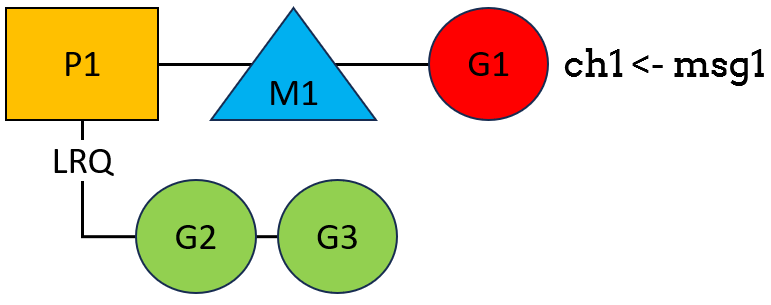
\includegraphics[scale=0.5]{figures/GoroutineChannel1.png}
	\caption{Channel-Kommunikation: G1 wird ausgeführt und blockiert}
	\label{fig:GoroutineChannel1}
\end{figure}

Auf der Abbildung ist die oben beschrieben Ausgangssituation zu sehen. P1 führt aktuell G1 aus. G1 möchte die Nachricht \texttt{msg1} an den Channel \texttt{ch1} senden. Da es aktuell keinen Empfänger gibt blockiert G1 und wechselt in den Status Waiting. Dies registriert der Scheduler und entnimmt G1 aus P1. Wie in der nächsten Abbildung deutlich wird.

\begin{figure}[h]
	\centering
	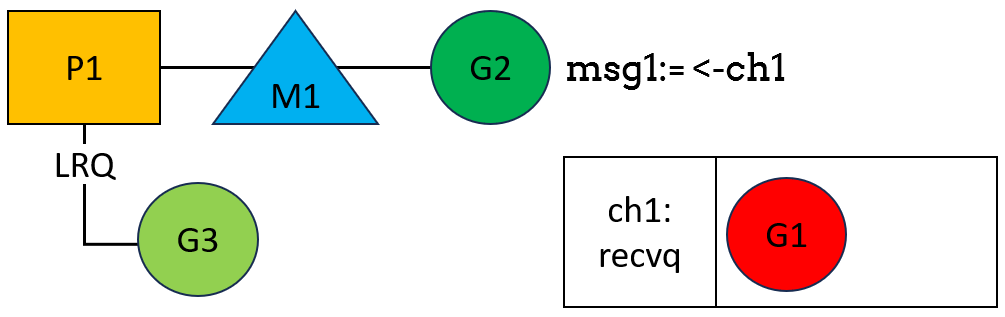
\includegraphics[scale=0.5]{figures/GoroutineChannel2.png}
	\caption{Channel-Kommunikation: G1 wird entfernt, G2 wird ausgeführt}
	\label{fig:GoroutineChannel2}
\end{figure}

Der Scheduler hat G1 aus P1 entfernt und Empfänger-Warteschlange \texttt{recvq} des Channels \texttt{ch1} zugewiesen. Dort wartet G1 auf einen Empfänger für die Nachricht. Da P1 jetzt keine Goroutine mehr ausführt entnimmt er die vorderste Goroutine aus seiner LRQ und beginnt mit der Bearbeitung. In diesem Fall ist dies G2. Dafür wird weiterhin der Betriebssystem Thread M1 genutzt der P1 bereits zugewiesen war. Der Status von G2 wird dementsprechend von runnable auf running geändert. G2 wiederum empfängt eine Nachricht vom Channel \texttt{ch1}, was zur Folge hat, dass G1 nicht länger blockiert ist. Zu sehen in der folgenden Abbildung.

\begin{figure}[h]
	\centering
	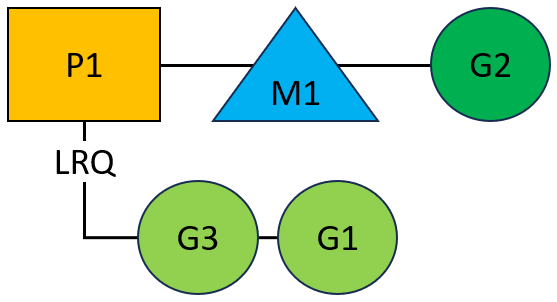
\includegraphics[scale=0.5]{figures/GoroutineChannel3.png}
	\caption{Channel-Kommunikation: G1 ist nicht mehr blockiert und wird in die LRQ verschoben}
	\label{fig:GoroutineChannel3}
\end{figure}

Da G2 die Nachricht von G1 empfangen hat ist G1 nicht mehr blockiert und wechselt auf den Status Runnable. Deshalb verschiebt der Scheduler G1 in die LRQ von P1.

Diese Beispiel hat verdeutlicht wie der Scheduler mit einer Goroutine umgeht die aufgrund von Channel-Kommunikation blockiert. In der Praxis hat ein System jedoch meist mehr als einen Prozessorkern, was dem Go-Scheduler zusätzliche Möglichkeiten zur Optimierung der Ausführung bietet. Dies wird im Abschnitt Workstealing(\ref{subsubsec:workstealing}) genauer erläutert.

\subsubsection{Systemaufrufe}

In dem folgenden Beispiel wird gezeigt wie der Scheduler mit Systemaufrufen innerhalb von Goroutinen umgeht. In diesem Beispiel gehen wir wieder von einem System mit einem Prozessorkern aus, deshalb gibt auch wieder nur einen logischen Prozessor P1. Dieser fürt die Goroutine G1 auf dem Betriebssystemthread M1 aus. Außerdem wartet eine zweite Goroutine G2 in derLRQ von P1 daruaf ausgeführt zu werden. Schlussendlich gibt es noch einen zweiten untätigen Betriebssystemthread M2 der aktuell nicht genutzt wird.

\begin{figure}[h]
	\centering
	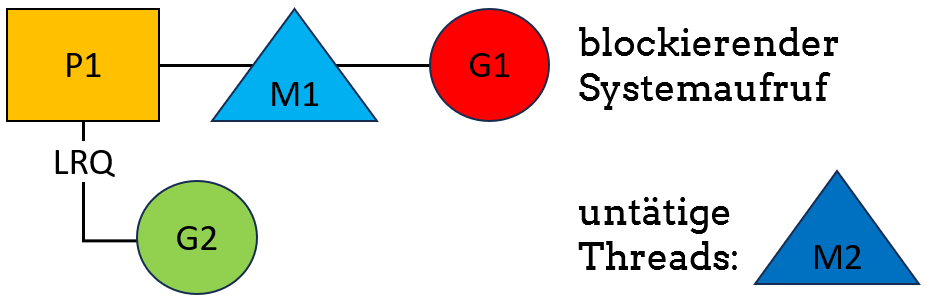
\includegraphics[scale=0.5]{figures/GoroutineSystemaufrufe1.png}
	\caption{Systemaufrufe: G1 ist auf Grund eines Systemaufrufs blockiert}
	\label{fig:GoroutineSystemaufrufe1}
\end{figure}

G1 führt einen Systemaufruf aus der dazu führt, dass G1 blockiert. Dies könnte zu beispielsweise eine I/O-Operation sein. Go hat keine direkte Kontrolle über die Ausführung von Systemaufrufen auf Betriebssystemebene. Sobald ein Systemaufruf initiiert wird, liegt die Kontrolle beim Betriebssystem. Deshalb blockiert nicht nur G1 sonder auch der ausführende Betriebssystemthread M1. Damit P1 weiterhin ausgelastet ist, werden sowohl G1 als auch M1 vom Scheduler freigegeben. P1 wird dann ein neuer Betriebssystemthread, in diesem Fall M2, zugewiesen und P1 kann die nächste Goroutine aus der LRQ ausführen, in diesem Fall G2.

\begin{figure}[h]
	\centering
	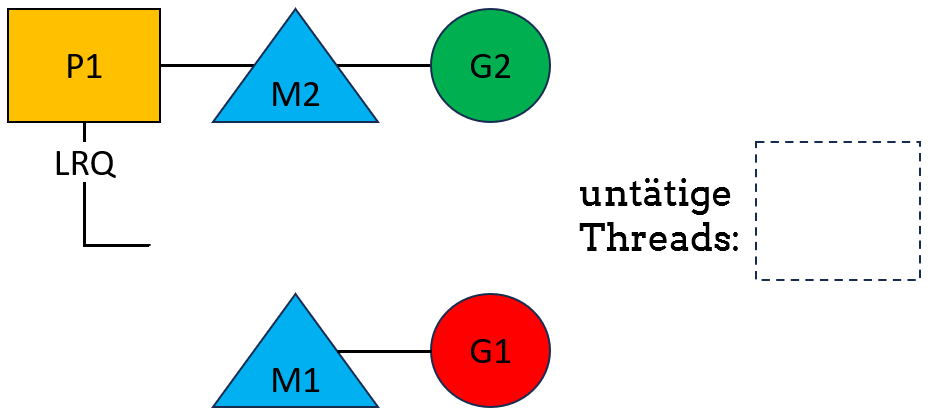
\includegraphics[scale=0.5]{figures/GoroutineSystemaufrufe2.png}
	\caption{Systemaufrufe: G1 wird mit M1 aus P1 entfernt, G2 wird auf M2 ausgeführt}
	\label{fig:GoroutineSystemaufrufe2}
\end{figure}

Wenn G1 nicht mehr blockiert ist, überprüft der Scheduler ob es einen freien logischen Prozessor gibt, der G1 auf M1 ausführen kann. In diesem Beispiel ist P1 aber mit der Ausführung von G2 beschäftigt. Deshalb wird G1 in die Global Run Queue (GRQ) verschoben. Dort gespeicherte Goroutinen werden von den logischen Prozessoren abgearbeitet sollte ihre eigene LRQ leer sein. M1 hingegen wird zu einem untätigen Thread.

\begin{figure}[h]
	\centering
	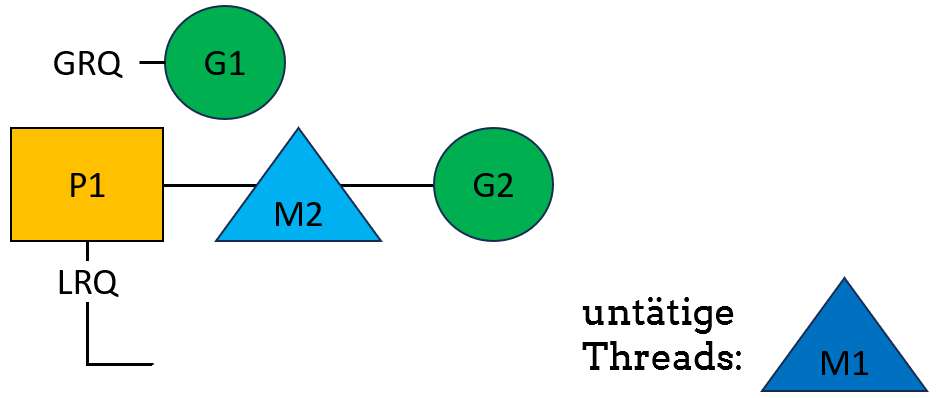
\includegraphics[scale=0.5]{figures/GoroutineSystemaufrufe3.png}
	\caption{G1 ist nicht mehr blockiert und wird in die GRQ verschoben}
	\label{fig:GoroutineSystemaufrufe3}
\end{figure}

Der Vorteil diese Verfahrens ist, dass die logischen Prozessoren nicht mit den Goroutinen blockieren. Sie können weiterhin Goroutinen ausführen. Jedoch wird für jeden Systemaufruf ein eigener Betriebssystemthread benötigt.

\subsubsection{Netzwerk-Kommunikation}

Eine weitere Kategorie von häufig blockierende Operationen ist die Kommunikation über Netzwerke. Für diesen Fall stellt Go den Net Poller\cite{netpoll2024} zur Verfügung. Er ist ein spezieller Goroutinen-Scheduler, der für die effiziente Verwaltung von Netzwerk-I/O-Operationen zuständig ist. Er nutzt betriebssystemspezifische Mechanismen wie \texttt{epoll} (Linux), \texttt{kqueue} (BSD) oder \texttt{IOCP} (Windows), um asynchrone I/O-Operationen zu ermöglichen.

Wenn eine Goroutine eine potenziell blockierende Netzwerkoperation durchführt (z.B. Lesen von einem Socket), übergibt sie die Kontrolle an den Net Poller. Der Net Poller registriert die Operation beim Betriebssystem und überwacht sie asynchron, ohne einen OS-Thread zu blockieren. Während der Net Poller auf die Fertigstellung der I/O-Operation wartet, kann der Go-Scheduler andere Goroutinen auf dem verfügbaren OS-Thread ausführen. Sobald die I/O-Operation abgeschlossen ist, benachrichtigt das Betriebssystem den Net Poller. Der Net Poller setzt die ursprüngliche Goroutine zur Ausführung fort, sobald ein Thread verfügbar ist.

Der Net Poller ermöglicht es, eine große Anzahl von gleichzeitigen Netzwerkverbindungen mit einer begrenzten Anzahl von Betriebssystemthreads zu verwalten. Durch die Vermeidung von blockierten Betriebssystemthreads wird die CPU-Auslastung optimiert. Programmierer können blockierende I/O-Operationen in Goroutinen schreiben, ohne sich um die zugrunde liegende asynchrone Implementierung kümmern zu müssen. Da der Net Poller tief in die Go-Laufzeitumgebung integriert ist. Er arbeitet eng mit dem Goroutine-Scheduler zusammen, um eine nahtlose Integration von Netzwerk-I/O und Goroutinen-Ausführung zu gewährleisten. 

\subsubsection{Work-Stealing}
\label{subsubsec:workstealing}

In diesem letzten Abschnitt soll gezeigt werden wie der Work-Stealing-Algorithmus im Goroutinen-Scheduler funktioniert. Er sorgt für eine effiziente Verteilung der Arbeitslast zwischen den verfügbaren logischen Prozessoren (P). Jeder Prozessor (P) hat eine eigene lokale Warteschlange (LRQ) für Goroutinen. Neue Goroutinen werden normalerweise in die lokale Warteschlange des erzeugenden P gelegt. Ein P arbeitet primär an Goroutinen aus seiner eigenen lokalen Warteschlange. In diesem Beispiel gibt es zwei Prozessorkerne und damit zwei logische Prozessoren P1 und P2. Diese arbeiten die ihnen zugewiesenen Goroutinen ab.

\begin{figure}[H]
	\centering
	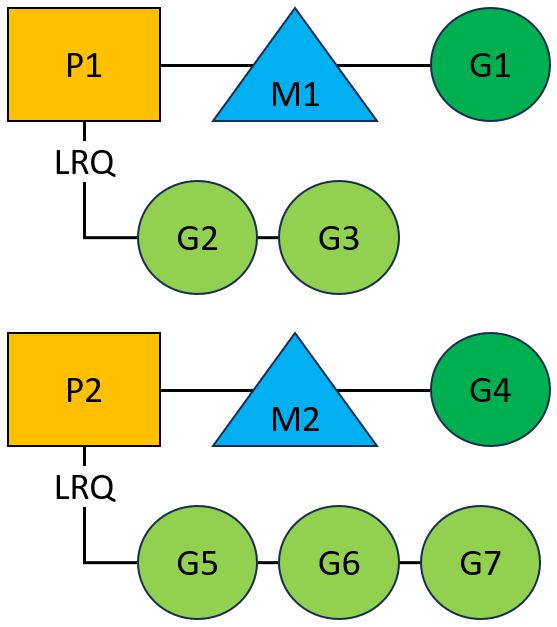
\includegraphics[scale=0.5]{figures/GoroutineWorkstealing1.png}
	\caption{Work-Stealing: P1 und P2 führen Gs aus und haben gefüllte LRQs}
	\label{fig:GoroutineWorkstealing1}
\end{figure}

Wenn ein P keine Goroutinen mehr in seiner LRQ hat, versucht er, Goroutinen zu ``stehlen''. Er wählt zufällig einen anderen P aus und versucht, Goroutinen aus dessen LRQ zu entnehmen. In diesem Fall hat P1 alle seine Goroutinen abgearbeitet währen P2 immer noch beschäftigt ist.

\begin{figure}[h]
	\centering
	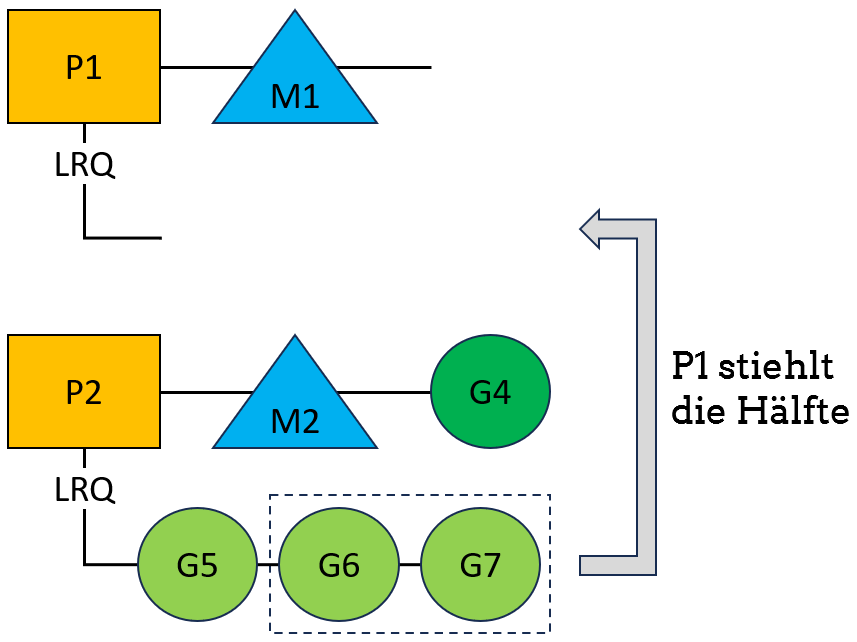
\includegraphics[scale=0.5]{figures/GoroutineWorkstealing2.png}
	\caption{Work-Stealing: P1 hat keine Gs mehr und stiehlt die Hälfte der Gs aus der LRQ von P2}
	\label{fig:GoroutineWorkstealing2}
\end{figure}

Deshalb stiehlt P1 die hintere Hälfte der LRQ von P2 und verschiebt sie in seine eigene LRQ. Wenn das Stehlen von anderen Ps nicht erfolgreich ist, greift der P auf die GRQ zurück.

Der Work-Stealing-Algorithmus ist ein Schlüsselelement, das zur hohen Effizienz und Skalierbarkeit von Go's Nebenläufigkeitsmodell beiträgt. Er ermöglicht es, eine große Anzahl von Goroutinen effizient auf einer begrenzten Anzahl von Betriebssystem-Threads zu verwalten.

\subsection{Goroutinen-Programmiermuster}

Um das volle Potenzial von Goroutinen auszuschöpfen und typische Herausforderungen der nebenläufigen Programmierung zu bewältigen, haben sich in der Go-Community verschiedene Programmiermuster (Pattern) etabliert. Die Verwendung dieser Muster trägt dazu bei, komplexe Probleme in überschaubare Teilaufgaben zu zerlegen und die Kommunikation zwischen Goroutinen zu strukturieren. Die im folgenden vorgestellten Programmiermuster stammen dabei aus den Vorträgen ''Go Concurrency Patterns''\cite{Pike2012} und ''Advanced Go Concurrency Patterns''\cite{Ajmani2013}.

\subsubsection{Generator-Programmiermuster}
\label{subsubsec:generator}

Das Generator-Muster ermöglicht das Erstellen von Funktionen, die Sequenzen von Werten produzieren, ohne alle Werte auf einmal im Speicher zu halten. Stattdessen werden die Werte bei Bedarf generiert und über einen Channel zurückgegeben. Bei dem folgenden Code-Beispiel handel es sich um eine Modifizierung des Codes aus dem Channel-Abschnitts (\ref{subsec:channel}).

\begin{lstlisting}[language=Go,extendedchars=true]
	package main
	
	import (
		"fmt"
	)

	// Generator-Funktion mit Namensparameter
	func helloCounter(name string) <-chan string {
		ch := make(chan string)
		//Starten der Goroutine
		go func() {
			for i := 0; i < 5; i++ {
				ch <- fmt.Sprintf("Hallo %s, %d!\n", name, i)
			}
			close(ch)
		}()
		return ch
	}

	func main() {
		philipp := helloGenerator("Philipp")
		michael := helloGenerator("Michael")
		for i := 0; i < 5; i++{
			fmt.Print(<-philipp)
			fmt.Print(<-michael)
		}
	}
\end{lstlisting}

Die auffälligste Veränderung ist, dass die Funktion \texttt{helloCounter} in der \texttt{main}-Funktion nicht mehr mit dem Schlüsselwort \texttt{go} als Goroutine gestartet werden muss. Stattdessen wird die Goroutine in der Funktion \texttt{helloCounter} intern gestartet. Außerdem wird auch der Channel von \texttt{helloCounter} erstellt und als Rückgabewert zurückgegeben. Das hat den Vorteil, dass sich leicht mehrere Instanzen der Generatorfunktion nebenläufigstarten lassen, wie im Beispiel gezeigt. Im Prinzip lässt sich eine Generatorfunktion als Service betrachten bei dem sich der Anwender nicht mehr um die Nebenläufigkeit kümmern muss, da sie bereits intern sichergestellt wurde.

\subsubsection{Fan-In-Programmiermuster}

Die Aufgabe einer Fan-In-Funktion ist es Ausgaben mehrerer Goroutinen zu sammeln und sie in einem einzigen Datenstrom zusammenzuführen. Durch die Zusammenführung mehrerer Datenströme in einem einzelnen Kanal wird die Verarbeitung der Ergebnisse effizienter gestaltet. In der Praxis wird die Fan-In-Funktion oft in Szenarien eingesetzt, wo Daten parallel verarbeitet werden müssen und die Ergebnisse anschließend zusammengeführt werden sollen, wie beispielsweise bei verteilten Berechnungen oder bei der Verarbeitung großer Datenmengen. Das nachfolgende Beispiel stellt eine Modifizierung des Codes aus dem Generator-Muster Abschnitt (\ref{subsubsec:generator}) dar.

\begin{lstlisting}[language=Go,extendedchars=true]
	func fanIn(ch1, ch2 <-chan string) <-chan string {
		new_ch := make(chan string)
		go func() {
			for {
				select {
					case s, ok := <-ch1:
					if !ok {
						ch1 = nil
						break
					}
					new_ch <- s
					case s, ok := <-ch2:
					if !ok {
						ch2 = nil
						break
					}
					new_ch <- s
				}
				if ch1 == nil && ch2 == nil {
					close(new_ch)
					return
				}
			}
		}()
		return new_ch
	}

	func main() {
		ch := fanIn(helloCounter("Philipp"), helloCounter("Michael"))
		for msg := range ch {
			fmt.Println(msg)
		}
	}
\end{lstlisting}

In dem Beispiel wurde der Code um eine Fan-In-Funktion erweiter. Dieser Funktion werden in der \texttt{main}-Funktion die beiden Channels der \texttt{helloCounter}-Funktionen übergeben. Die Aufgabe der Fan-In-Funktion ist es, die Ausgaben der beiden Channels zusammenzufassen und in einem neuen Channel (\texttt{new\_ch}) gebündelt an die \texttt{main}-Funktion weiter zugeben. Dafür wird in der Fan-In-Funktion das Generator-Muster verwendet. Es wird innerhalb der Funktion eine Goroutine gestartet. In der Goroutine wird eine \texttt{select}-Anweisung verwendet um auf beiden Channels parallel auf eine Antwort zu warten. Diese Antworten werden dann auf den \texttt{new\_ch} weiter geleitet. Dies geschieht so lange bis beide Channels der \texttt{helloCounter}-Funktionen geschlossen sind. Dann wird auch der \texttt{new\_ch} geschlossen. Der Vorteil der Verwendung einer Fan-In-Funktion in der \texttt{main}-Funktion, wird schnell deutlich. Es ist möglich nun mehrere Nachrichten hintereinander von der gleichen \texttt{helloCounter}-Funktionen zu empfangen. Außerdem muss in der \texttt{main}-Funktion auch nur noch ein Channel verarbeitet werden. 

Als Gegenstück zum Fan-In-Muster gibt es das Fan-Out-Muster. Bei diesem werden Nachrichten aus einer einzelnen Quelle auf mehrere Goroutinen verteilt.

\subsubsection{Closing Channels-Programmiermuster}
\label{subsubsec:closingchannel}

Das Closing Channels-Muster ist ein wichtiges Konzept in Go, um Goroutinen sauber zu beenden und Ressourcen freizugeben. Das grundlegende Prinzip lautet: Der Sender eines Channels sollte den Channel schließen, nicht der Empfänger. Dies verhindert Ausnahmen (Panic) durch das Senden auf bereits geschlossene Kanäle. Das folgende Beispiel zeigt eine mögliche Implementierung des Closing Channels-Muster:

\begin{lstlisting}[language=Go,extendedchars=true]
package main

import (
"fmt"
"time"
)

func worker(id int, done <-chan struct{}, c <-chan int) {
	for {
		select {
			case <-done:
			fmt.Printf("Worker %d: Beende Arbeit\n", id)
			return
			case value := <-c:
			fmt.Printf("Worker %d: Verarbeite Wert %d\n", id, value)
			time.Sleep(time.Second) // Simuliere Verarbeitungszeit
		}
	}
}

func main() {
	done := make(chan struct{}) // Closing Channel
	c := make(chan int)
	
	// Starte drei Worker
	for i := 1; i <= 3; i++ {
		go worker(i, done, c)
	}
	
	// Sende Werte an die Worker
	for i := 1; i <= 5; i++ {
		c <- i
		fmt.Printf("Hauptroutine: Sende Wert %d\n", i)
		time.Sleep(500 * time.Millisecond) // Kurze Pause zwischen den Sendungen
	}
	
	fmt.Println("Hauptroutine: Beende alle Worker")
	close(done) // Signal zum Beenden senden
	
	// Warte kurz, damit die Worker-Ausgaben sichtbar sind
	time.Sleep(2 * time.Second)
}
\end{lstlisting}

In der \texttt{main}-Funktion wird ein neuer separater Channel mit dem Namen \texttt{done} erstellt, dies ist der so genannte Closing Channel. Danach werden drei \texttt{worker}-Goroutinen gestartet. Diese erhalten Werte über den Channel \texttt{c} und sie auf der Konsole aus. Nachdem die Hauptroutine alle Werte gesendet hat schließt sie den Closing Channel. Dies Signalisiert \texttt{worker}-Goroutinen, dass keine weiteren Werte gesendet werden und sie beenden sich selbst.

\subsection{Zusammenfassung}

Abschließend läss sich zusammenfassen, bei Goroutinen handelt es sich um leichtgewichtige Threads, die nebenläufige Ausführungen ermöglichen. Sie lassen sich durch das Schlüsselwort \texttt{go} starten und laufen unabhängig von der Hauptfunktion, wobei sie einen gemeinsamen Adressraum teilen. Die Kommunikation und Synchronisation zwischen Goroutinen erfolgt über Channels, die den sicheren Datenaustausch ermöglichen. Die Go-Laufzeitumgebung enthält einen Scheduler, der Goroutinen effizient verwaltet. Um eine ausgewogene Auslastung der Prozessoren zu gewährleisten, nutzt der Scheduler verschiedene Warteschlangen(LRQ und GRQ) und einen Work-Stealing-Algorithmus. Verschiedene Programmiermuster, wie das Fan-In-Muster und das gezielte Schließen von Channels, unterstützen eine strukturierte Handhabung der Nebenläufigkeit und optimieren die Gesamtleistung der Programme.

\section{Vergleich der Konzepte}

Im folgendem werden die Erkenntnisse die über Java Platform Threads, Java Virtual Threads, Kotlin Coroutinen und Go Goroutinen gesammelt wurden, miteinander verglichen, um so sowohl Gemeinsamkeiten als auch Unterschiede hervorzuheben.

\subsubsection{Unterstützte Sprachen}

Platform Threads sind in Java, Kotlin und anderen JVM-Sprachen verfügbar, was ihre breite Anwendbarkeit unterstreicht. Virtual Threads hingegen sind eine neuere Entwicklung und stehen ab Java Version 21 zur Verfügung. Kotlin Coroutinen sind spezifisch für die Kotlin-Sprache konzipiert, während Goroutinen exklusiv in Go implementiert sind.

\subsubsection{Ausführungskontrolle und Blockierverhalten}

Der Mechanismus zur Ausführungskontrolle variiert stark zwischen den Konzepten. Platform Threads nutzen betriebssystembasiertes Scheduling, was zu einer direkten Blockierung des BS-Threads führt. Im Gegensatz dazu verwenden Virtual Threads, Coroutinen und Goroutinen fortschrittlichere Mechanismen, die es ermöglichen, den BS-Thread freizugeben, wenn eine Operation blockiert. Virtual Threads und Kotlin Coroutinen basieren auf Continuations, während Go einen eigenen Goroutinen-Scheduler implementiert.

\subsubsection{Thread-Pool-Nutzung und Ressourcenverbrauch}

Bei der Thread-Pool-Nutzung zeigen sich Unterschiede: Platform Threads und Coroutinen erfordern eine explizite Nutzung, während Virtual Threads und Goroutinen dies implizit handhaben. Der Ressourcenverbrauch ist bei Platform Threads deutlich höher (schwergewichtig), während die anderen drei Konzepte als leichtgewichtig gelten.

\subsubsection{Stackgröße und maximale Anzahl}

Die Stackgröße variiert erheblich, von großen Stacks bei Platform Threads (oft 1 MB oder mehr) bis zu sehr kleinen bei Virtual Threads und Go Goroutinen. Kotlin Coroutinen nutzen keinen eigenen Stack, sondern den Hauptstack kurzzeitig. Diese Unterschiede wirken sich direkt auf die maximale Anzahl aus, die bei Platform Threads einige tausend begrenzt, bei den anderen Konzepten jedoch mit mehreren Millionen sehr hoch ist.

\subsubsection{Synchronisationsmechanismen}

Die Synchronisationsmechanismen reichen von klassischen Locks, Monitoren und Futures bei Platform und Virtual Threads bis zu spezialisierten Konzepten wie suspend und Scope bei Kotlin Coroutinen oder Channels bei Go Goroutinen. 

\subsubsection{Anwenderfreundlichkeit}

Die Bewertung der Anwenderfreundlichkeit ist subjektiv und kann je nach Nutzer unterschiedlich ausfallen. 

Platform und Virtual Threads werden als einfach  eingestuft. Sie nutzen beide das bekannte Thread-Modell von Java und haben haben mit dem ExecutorService eine einheitliche API die nur wenig konfiguriert werden muss. 

Kotlin Coroutinen werden was die Anwenderfreundlichkeit betrifft als mittel eingeschätzt, da sie viele neue Begriffe einführen die vorher nicht geläufig waren. Außerdem ist der Konfigurationsaufwand größer und bietet mehr Möglichkeiten für Fehler, zum Beispiel mit der richtigen Wahl des Builders oder Dispatchers. 

Auch Go Goroutinen werden als mittel bewertet. Zwar werden für die Nutzung nur wenige Schlüsselwörter benötige. Für einen effizienten Einsatz von Goroutinen sollte ein Entwickler aber auch die in dieser Arbeit vorgestellten Programmiermuster kennen, was sie deutlich weniger einsteigerfreundlich macht.

\begin{table}[h]
	\centering
	\renewcommand{\arraystretch}{1.2}
	\begin{tabularx}{\textwidth}{L{4cm}Y Y Y Y}
		\toprule
		\rowcolor{gray!20}
		\textbf{Eigenschaft} & \textbf{\makecell[l]{Java \\ Platform \\ Threads}} & \textbf{\makecell[l]{Java \\ Virtual \\ Threads}} & \textbf{\makecell[l]{Kotlin \\ Coroutinen}} & \textbf{\makecell[l]{Go \\ Goroutinen}} \\
		\midrule
		Unterstützte Sprachen & Java, Kotlin, JVM-Sprachen & Java (ab Version 21) & Kotlin & Go \\
		\rowcolor{gray!10}
		Mechanismus zur Ausführungskontrolle & BS-basiertes Scheduling & Continuations (Scheduling durch JVM) & Continuations (Kotlin Runtime) & Goroutinen-Scheduler (Go Runtime) \\
		Blockierverhalten & Blockiert BS-Thread & Gibt BS-Thread frei & Gibt BS-Thread frei & Gibt BS-Thread frei \\
		\rowcolor{gray!10}
		Thread-Pool-Nutzung & Explizit & Implizit & Explizit (Dispatcher) & Implizit \\
		Ressourcenverbrauch & \makecell[l]{Schwer-\\gewichtig} & \makecell[l]{Leicht-\\gewichtig} & \makecell[l]{Leicht-\\gewichtig} & \makecell[l]{Leicht-\\gewichtig} \\
		\rowcolor{gray!10}
		Stackgröße & Groß (oft 1 MB oder mehr) & Klein (oft ein paar KB) & Kein eigener Stack, nutzt Hauptstack kurz & Klein (einige KB, wächst dynamisch) \\
		Maximale Anzahl & Begrenzt & Hoch & Sehr hoch & Sehr hoch \\
		\rowcolor{gray!10}
		\makecell[l]{Synchronisations-\\mechanismen} & Locks, Monitore, Future & Locks, Monitore, Future & suspend, Scope & Channels \\
		Anwenderfreundlichkeit & Einfach & Einfach & Mittel & Mittel \\
		\bottomrule
	\end{tabularx}
	\caption{\textbf{Vergleich von Thread-Abstraktionen in verschiedenen Programmiersprachen}}
	\label{tab:thread-comparison}
\end{table}

\chapter{Testaufbau}

Das folgende Kapitel beschreibt den Testaufbau für die praktische Umsetzung der Leistungsanalyse der verschiedener Thread-Abstraktionen in Java, Kotlin und Go. 

Um eine fundierte und aussagekräftige Bewertung der Per\-for\-mance\-un\-ter\-schiede zu erzielen, wurde ein sorgfältig konzipierter Testaufbau entwickelt. Dieser Aufbau gewährleistet nicht nur die Vergleichbarkeit der Ergebnisse zwischen den verschiedenen Programmiersprachen und ihren Thread-Implementierungen, sondern stellt auch die Reproduzierbarkeit der Messungen sicher.

In den folgenden Abschnitten  zunächst die verwendete Testumgebung, einschließlich der Hardware- und Software-Konfiguration, beschrieben. Anschließend werden die für die Leistungsanalyse relevanten Performancefaktoren erläutert und begründet. Diese Faktoren bilden die Grundlage für die quantitative Bewertung der verschiedenen Thread-Abstraktionen. Abschließend werden die speziell für diese Untersuchung entwickelten Werkzeuge zur Datenerhebung vorgestellt. Diese maßgeschneiderten Tools ermöglichen eine präzise und konsistente Erfassung der Leistungsdaten über alle getesteten Implementierungen hinweg.

\section{Testumgebung}

Um eine konsistente und reproduzierbare Testumgebung für die Leistungsanalyse der verschiedenen Thread-Abstraktionen zu gewährleisten, wurde eine spezifische Hard- und Software-Konfiguration verwendet. Diese Konfiguration wurde für alle durchgeführten Benchmarks beibehalten, um vergleichbare Ergebnisse zu erzielen.

Alle Tests wurden in einer kontrollierten Umgebung durchgeführt, wobei darauf geachtet wurde, dass keine anderen ressourcenintensiven Prozesse parallel liefen. Das System wurde vor jedem Testlauf neu gestartet, um konsistente Ausgangsbedingungen zu gewährleisten. Zudem wurden alle Netzwerkverbindungen deaktiviert, um mögliche Interferenzen durch externe Faktoren zu minimieren.

\subsection{Hardware}

\begin{itemize}
	\item \textbf{Prozessor:} Intel(R) Core(TM) i5-8300H CPU @ 2.30GHz
	\item[] \hspace{0.8cm}\textbf{Kerne:} 4 physische Kerne, 8 logische Prozessoren
	\item[] \hspace{0.8cm}\textbf{Basistakt:} 2.30GHz
	\item \textbf{Arbeitsspeicher:} 16,0 GB (15,9 GB verwendbar)
	\item \textbf{Festplatte:} SSD 256 GB
\end{itemize}

\subsection{Software}

\begin{itemize}
	\item \textbf{Betriebssystem:} Microsoft Windows 11 Home (Version 26100.2161, 64-Bit)
	\item \textbf{Java Development Kit (JDK):} xxx
	\item \textbf{Kotlin:} xxx
	\item \textbf{Go:} xxx
\end{itemize}

Docker

Python

%TODO:aktuelle Versionen

\section{Performancefaktoren}

Bei der Analyse und dem Vergleich verschiedener Thread-Abstraktionen ist es entscheidend, aussagekräftige und messbare Kriterien heranzuziehen. Diese Kriterien, die als Performancefaktoren bezeichnet werden, ermöglichen eine objektive Bewertung der Leistungsfähigkeit und Effizienz der unterschiedlichen Implementierungen. In dieser Masterarbeit liegt der Fokus auf vier Faktoren: Zeitmessung, CPU-Auslastung, Arbeitsspeicherverbrauch und Thread-Anzahl. Jeder dieser Faktoren beleuchtet einen spezifischen Aspekt der Leistung und trägt zu einem umfassenden Verständnis der Stärken und Schwächen der jeweiligen Thread-Abstraktionen bei. Die Performancefaktoren ermöglichen es, die Effizienz, Skalierbarkeit und Ressourcennutzung der verschiedenen Thread-\-Imple\-mentie\-rungen detailliert zu untersuchen und zu vergleichen. Im Folgenden wird jeder dieser Faktoren genauer betrachtet und erläutert:

\subsubsection{Zeitmessung}

Die Ausführungszeit ist einer der wichtigsten Indikatoren für die Leistungsfähigkeit der Thread-Abstraktionen. Durch präzise Zeitmessungen können verschiedene Implementierungen objektiv miteinander verglichen werden, um die effizienteste Lösung zu identifizieren. In der Praxis ist die Einhaltung von zeitlichen Vorgaben in Systemen mit Echtzeitanforderungen kritisch. Durch Zeitmessungen mit unterschiedlichen Eingabegrößen oder Lastszenarien kann die Skalierbarkeit eines Systems analysiert werden. So lässt sich abschätzen, wie sich die Leistung bei wachsenden Anforderungen entwickelt.

\subsubsection{CPU-Auslastung}

Die CPU-Auslastung gibt direkten Aufschluss darüber, wie effizient die verfügbaren Prozessorressourcen von den Threads genutzt werden. Eine hohe Auslastung deutet auf eine gute Ausnutzung der Rechenkapazität hin, während eine niedrige Auslastung auf Ineffizienzen oder Engpässe in anderen Bereichen hinweisen kann. Durch die Analyse der CPU-Auslastung lässt sich der Grad der Parallelisierung eines multithreaded Systems beurteilen. Eine gleichmäßige Auslastung über mehrere Kerne hinweg zeigt, dass die Arbeitslast effektiv auf die verfügbaren Ressourcen verteilt wird.

\subsubsection{Arbeitsspeicherverbrauch}

Ein effizienter Umgang mit dem Arbeitsspeicher ist entscheidend für die Gesamtleistung eines multithreaded Programms. Jeder Thread benötigt Speicher für seinen Stack und andere thread-spezifische Daten. Ein hoher Speicherverbrauch kann zu einer Verlangsamung des Systems führen und die Anzahl der möglichen gleichzeitigen Threads begrenzen. Der Speicherverbrauch beeinflusst direkt die Skalierbarkeit eines multithreaded Programms. Ein geringer Speicherverbrauch pro Thread ermöglicht mehr gleichzeitige Threads, während ein hoher Speicherbedarf die maximale Anzahl der Threads und damit die Parallelisierung limitiert. Schließlich schont ein effizienter Speicherverbrauch die Systemressourcen, indem mehr verfügbarer Speicher für andere Prozesse und den Betriebssystem-Cache bleibt und die Belastung des Speichermanagements des Betriebssystems geringer ausfällt.

\subsubsection{Thread-Anzahl}

Die Anzahl der Betriebssystemthreads ist ein bedeutender Performancefaktor bei der Messung der Benchmarks. Betriebssystemthreads sind eine begrenzte Ressource. Jeder Thread benötigt Speicher und andere Systemressourcen, was bedeutet, dass eine zu hohe Anzahl von Threads zu Ressourcenengpässen führen und die Gesamtleistung des Systems beeinträchtigen kann. Mit steigender Anzahl von Threads erhöht sich auch der Aufwand für das Betriebssystem, diese zu verwalten und zu planen. Dieser erhöhte Scheduling-Overhead kann zu einem höheren CPU-Verbrauch für Verwaltungsaufgaben und häufigeren Kontextwechseln führen, was die Effizienz des Gesamtsystems beeinträchtigt. Ab einem bestimmten Punkt kann eine Erhöhung der Threadanzahl sogar zu Leistungseinbußen führen, da die Threads um begrenzte Ressourcen konkurrieren.

\section{Werkzeuge zur Datenerhebung}

Für die Durchführung der Benchmarks und die Erhebung der relevanten Performancedaten wurden zwei speziell für diese Masterarbeit entwickelten Python-Skripte verwendet. Diese Skripte ermöglichen eine präzise und konsistente Messung der Leistungsparameter über alle getesteten Thread-Abstraktionen hinweg.

\subsubsection{monitoring}
%TODO: Richtigen Namen einsetzen

TODO:...

\subsubsection{plotting}
%TODO: Richtigen Namen einsetzen

TODO:...

\chapter{Benchmarks}

\section{Benchmark 1: Mergesort}

\subsection{Motivation: Mergesort}
Mergesort eignet sich hervorragend als Benchmark für den Vergleich verschiedener Thread-Abstraktionen. Der Algorithmus basiert auf dem Teile-und-herrsche-Prinzip, was eine natürliche Parallelisierung ermöglicht. Durch seine rekursive Struktur lässt sich Mergesort in kleinere, unabhängige Teilaufgaben zerlegen, die ideal für die parallele Verarbeitung geeignet sind. Dies macht den Algorithmus zu einem aussagekräftigen Testfall für die Effizienz und Skalierbarkeit verschiedener Nebenläufigkeitsimplementierungen.

Ein weiterer Vorteil von Mergesort als Benchmark ist seine vorhersehbare Zeitkomplexität von $\Theta(n\log{}n)$ für alle Eingabegrößen. Diese Eigenschaft ermöglicht es, die Leistung der verschiedenen Thread-Abstraktionen unter kontrollierten Bedingungen zu vergleichen. Zudem erfordert Mergesort sowohl Rechenoperationen als auch Speicherzugriffe, was eine umfassende Bewertung der Leistungsfähigkeit der untersuchten Technologien erlaubt.

Die Wahl von Mergesort als Benchmark bietet auch praktische Relevanz, da der Algorithmus häufig in realen Anwendungen zum Einsatz kommt, insbesondere bei der Verarbeitung großer Datenmengen. Somit können die gewonnenen Erkenntnisse direkt auf praxisnahe Szenarien übertragen werden. Durch die Verwendung von Mergesort als Benchmark lassen sich wertvolle Einblicke in die Stärken und Schwächen der verschiedenen Thread-Abstraktionen und Nebenläufigkeitskonzepte gewinnen, was für die Auswahl der geeigneten Technologie in spezifischen Anwendungsfällen von großer Bedeutung ist.

\subsection{Theoretische Grundlagen: Mergesort}

Mergesort ist ein effizienter, auf dem Prinzip "Teile und herrsche" basierender Sortieralgorithmus. Er wurde 1945 von John von Neumann entwickelt und zeichnet sich durch seine stabile Sortierung und vorhersagbare Leistung aus.

\subsubsection{Funktionsweise}

Der Mergesort-Algorithmus lässt sich in zwei Hauptphasen unterteilen: die Teilungsphase und die Zusammenführungsphase.

In der Teilungsphase wird die zu sortierende Liste rekursiv in immer kleinere Teillisten zerlegt, bis jede Teilliste nur noch ein Element enthält. Dies geschieht, indem die Liste in der Mitte geteilt wird, wodurch zwei etwa gleich große Hälften entstehen.

In der Zusammenführungsphase werden die sortierten Teillisten schrittweise wieder zusammengeführt. Dabei werden jeweils zwei benachbarte, sortierte Teillisten zu einer größeren sortierten Liste verschmolzen. Dieser Prozess wird fortgesetzt, bis die gesamte Liste sortiert ist.

Die rekursive Natur des Mergesort-Algorithmus lässt sich anschaulich als Baumstruktur darstellen, die während der Teilungsphase entsteht. Die Wurzel des Baums repräsentiert die ursprüngliche, unsortierte Liste. Jeder innere Knoten stellt eine Teilung der Liste dar. Die Blätter des Baums sind die einzelnen Elemente der Liste. Die Tiefe des Baums entspricht der Anzahl der rekursiven Teilungen, die durchgeführt werden müssen, um zu einzelnen Elementen zu gelangen. Sie beträgt etwa $\log_2(n)$, wobei $n$ die Anzahl der Elemente in der ursprünglichen Liste ist.

Beim Aufstieg im Baum, also während der Zusammenführungsphase, werden die sortierten Teillisten schrittweise verschmolzen. Jede Ebene im Baum repräsentiert dabei einen Schritt im Sortierprozess, bei dem längere sortierte Sequenzen entstehen.

Diese Baumstruktur verdeutlicht nicht nur die Arbeitsweise des Algorithmus, sondern auch sein Parallelisierungspotenzial: Unterschiedliche Zweige des Baums können unabhängig voneinander bearbeitet werden, was eine effiziente parallele Implementierung ermöglicht.

\subsubsection{Komplexität}

Mergesort weist in allen Fällen (Best-Case, Average-Case und Worst-Case) eine Zeitkomplexität von $\Theta(n \log n)$ auf, wobei $n$ die Anzahl der zu sortierenden Elemente ist. Dies macht Mergesort zu einem sehr effizienten Sortieralgorithmus, insbesondere für große Datenmengen. Außerdem sind dies sehr gute Voraussetzungen für die Eignung als Benchmark, da die Zeitliche Performance nicht von dem Inhalt der zu verarbeitenden Daten abhängt.\cite{Cormen2022}

Die Speicherkomplexität von Mergesort beträgt $\Theta(n)$, da zusätzlicher Speicherplatz für die temporären Teillisten benötigt wird. Dies kann bei sehr großen Datenmengen zu einem Nachteil werden.

\subsubsection{Parallelisierbarkeit}

Ein bedeutender Vorteil von Mergesort ist seine hervorragende Eignung für die Parallelisierung. Sowohl die Teilungs- als auch die Zusammenführungsphase können parallel ausgeführt werden, was den Algorithmus besonders effizient für Mehrprozessorsysteme macht.

In der Teilungsphase können die rekursiven Aufrufe zur Sortierung der Teillisten unabhängig voneinander auf verschiedenen Threads ausgeführt werden.

In der Zusammenführungsphase kann das Verschmelzen der sortierten Teillisten ebenfalls parallel erfolgen, was die Gesamtleistung weiter verbessert.
Diese Eigenschaften machen Mergesort zu einem idealen Kandidaten für die Implementierung mit verschiedenen Thread-Abstraktionen und Nebenläufigkeitskonzepten, was ihn zu einem wertvollen Benchmark für den Vergleich dieser Technologien macht.

\subsection{Implementierung: Mergesort}

\subsubsection{Basisimplementierung: Mergesort}

\subsubsection{Virtual Threads: Mergesort}

\subsubsection{Platform Threads: Mergesort}

\subsubsection{Coroutinen: Mergesort}

\subsubsection{Goroutinen: Mergesort}

global scope doppelt so schnell

\subsection{Messungen: Mergesort}

\subsubsection{Messung 1: Mergesort - Baumebenen:1-6}

\begin{figure}[H]
	\centering
	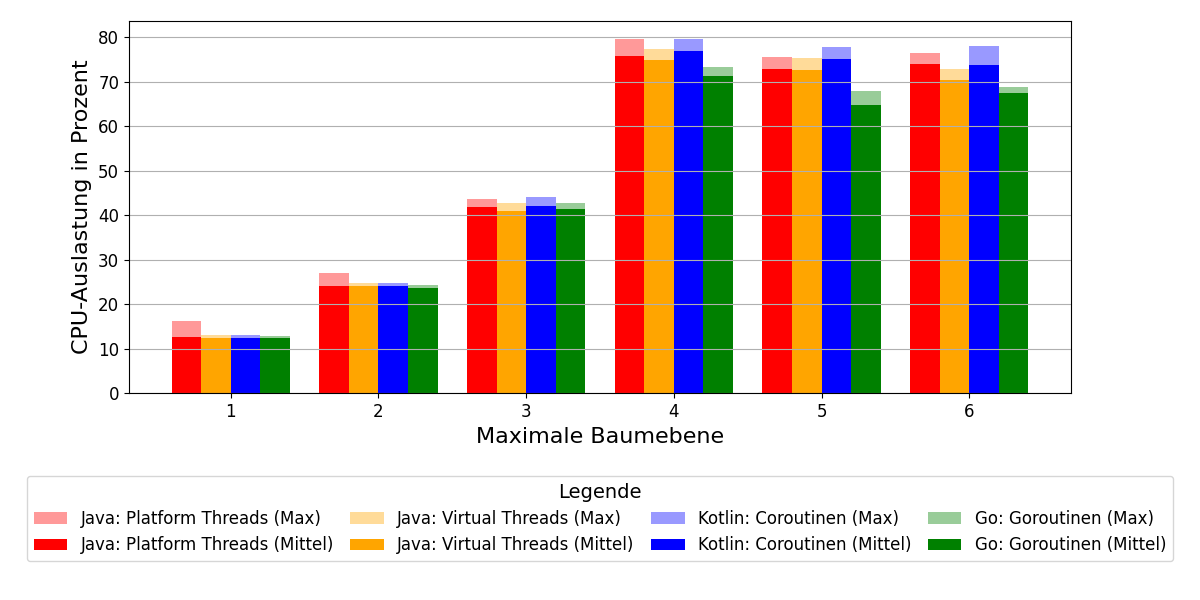
\includegraphics[scale=0.5]{figures/mergesort/Maximalebauebenen1-6/cpu_usage_bar_plot.png}
	\caption{Mergesort max. Baumebenen:1-6: CPU-Auslastung}
	\label{fig:ms1-6CPU}
\end{figure}

\begin{table}[h]
	\centering
	\renewcommand{\arraystretch}{1.2} % Erhöhte Zeilenhöhe
	\rowcolors{2}{gray!10}{white} % Alternierende Zeilenfarben ab der zweiten Zeile
	\begin{tabularx}{\textwidth}{XXXXXXXXX} % 9 gleichmäßig verteilte Spalten
		\toprule
		\rowcolor{gray!20} % Kopfzeile farbig
		\textbf{\makecell[l]{Max \\ Baum- \\ ebene}} & 
		\textbf{\makecell[l]{JVT \\ Max \\ CPU}} & 
		\textbf{\makecell[l]{JVT \\ Mittel \\ CPU}} & 
		\textbf{\makecell[l]{JPT \\ Max \\ CPU}} & 
		\textbf{\makecell[l]{JPT \\ Mittel \\ CPU}} & 
		\textbf{\makecell[l]{Coro\\ Max \\ CPU}} & 
		\textbf{\makecell[l]{Coro\\ Mittel \\ CPU}} & 
		\textbf{\makecell[l]{Goro\\ Max \\ CPU}} & 
		\textbf{\makecell[l]{Goro\\ Mittel \\ CPU}} \\
		\midrule
		\csvreader[
		head to column names,
		late after line=\\
		]{measurements/mergesort/Maximalebauebenen1-6/cpu_usage_aggregated.csv}{}
		{\csvcoli & 
			\pgfmathparse{\csvcolii}\pgfmathprintnumber{\pgfmathresult}\% & 
			\pgfmathparse{\csvcoliii}\pgfmathprintnumber{\pgfmathresult}\% & 
			\pgfmathparse{\csvcoliv}\pgfmathprintnumber{\pgfmathresult}\% & 
			\pgfmathparse{\csvcolv}\pgfmathprintnumber{\pgfmathresult}\% & 
			\pgfmathparse{\csvcolvi}\pgfmathprintnumber{\pgfmathresult}\% & 
			\pgfmathparse{\csvcolvii}\pgfmathprintnumber{\pgfmathresult}\% & 
			\pgfmathparse{\csvcolviii}\pgfmathprintnumber{\pgfmathresult}\% & 
			\pgfmathparse{\csvcolix}\pgfmathprintnumber{\pgfmathresult}\%}
		\bottomrule
	\end{tabularx}
	\caption{\textbf{Mergesort max. Baumebenen 1-6: CPU-Auslastung}}
	\label{tab:ms1-6CPU}
\end{table}

\begin{figure}[H]
	\centering
	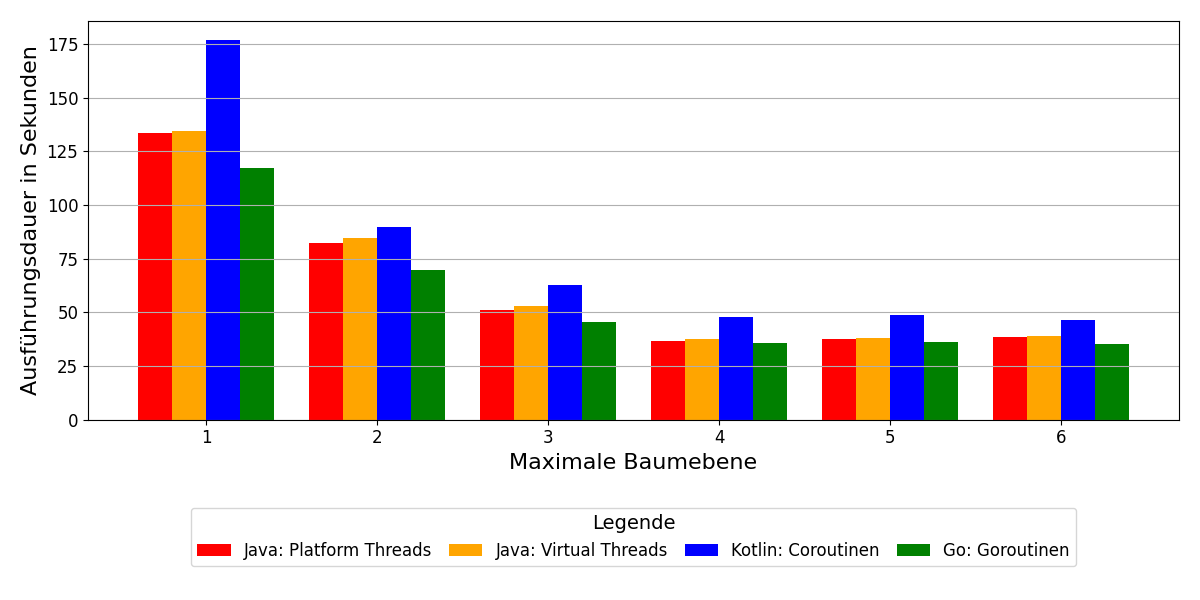
\includegraphics[scale=0.5]{figures/mergesort/Maximalebauebenen1-6/execution_time_plot.png}
	\caption{Mergesort max. Baumebenen:1-6: Ausführungszeit}
	\label{fig:ms1-6Zeit}
\end{figure}

\begin{table}[h]
	\centering
	\renewcommand{\arraystretch}{1.2} % Erhöhte Zeilenhöhe
	\rowcolors{2}{gray!10}{white} % Alternierende Zeilenfarben ab der zweiten Zeile
	\begin{tabularx}{\textwidth}{XXXXX} % 9 gleichmäßig verteilte Spalten
		\toprule
		\rowcolor{gray!20} % Kopfzeile farbig
		\textbf{\makecell[l]{Max \\ Baum- \\ ebene}} & 
		\textbf{\makecell[l]{JVT \\ Zeit \\ Gesamt}} & 
		\textbf{\makecell[l]{JPT \\ Zeit \\ Gesamt}} & 
		\textbf{\makecell[l]{Coro\\ Zeit \\ Gesamt}} & 
		\textbf{\makecell[l]{Goro\\ Zeit \\ Gesamt}} \\
		\midrule
		\csvreader[
		head to column names,
		late after line=\\
		]{measurements/mergesort/Maximalebauebenen1-6/execution_time_aggregated.csv}{}
		{\csvcoli & 
			\pgfmathparse{\csvcolii}\pgfmathprintnumber{\pgfmathresult} s & 
			\pgfmathparse{\csvcoliii}\pgfmathprintnumber{\pgfmathresult} s & 
			\pgfmathparse{\csvcoliv}\pgfmathprintnumber{\pgfmathresult} s & 
			\pgfmathparse{\csvcolv}\pgfmathprintnumber{\pgfmathresult} s}
		\bottomrule
	\end{tabularx}
	\caption{\textbf{Mergesort max. Baumebenen:1-6: Ausführungszeit}}
	\label{tab:ms1-6Zeit}
\end{table}

\begin{figure}[H]
	\centering
	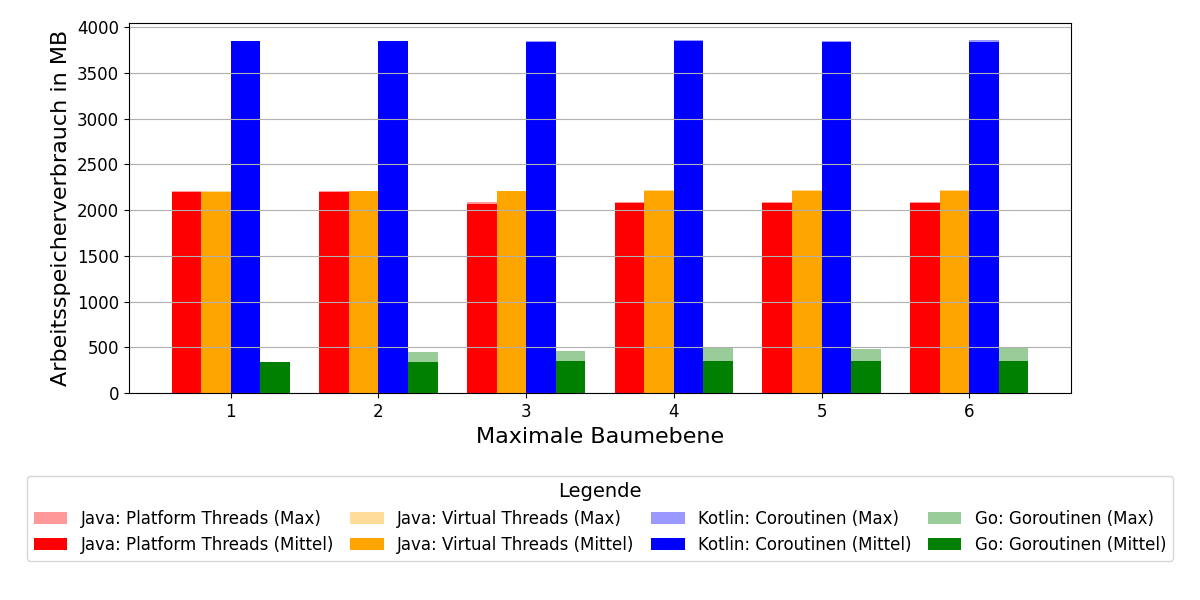
\includegraphics[scale=0.5]{figures/mergesort/Maximalebauebenen1-6/memory_usage_bar_plot.png}
	\caption{Mergesort max. Baumebenen:1-6: Arbeitsspeicherverbrauch}
	\label{fig:ms1-6RAM}
\end{figure}

\begin{table}[h]
	\centering
	\renewcommand{\arraystretch}{1.2} % Erhöhte Zeilenhöhe
	\rowcolors{2}{gray!10}{white} % Alternierende Zeilenfarben ab der zweiten Zeile
	\begin{tabularx}{\textwidth}{XXXXXXXXX} % 9 gleichmäßig verteilte Spalten
		\toprule
		\rowcolor{gray!20} % Kopfzeile farbig
		\textbf{\makecell[l]{Max \\ Baum- \\ ebene}} & 
		\textbf{\makecell[l]{JVT \\ Max \\ RAM}} & 
		\textbf{\makecell[l]{JVT \\ Mittel \\ RAM}} & 
		\textbf{\makecell[l]{JPT \\ Max \\ RAM}} & 
		\textbf{\makecell[l]{JPT \\ Mittel \\ RAM}} & 
		\textbf{\makecell[l]{Coro\\ Max \\ RAM}} & 
		\textbf{\makecell[l]{Coro\\ Mittel \\ RAM}} & 
		\textbf{\makecell[l]{Goro\\ Max \\ RAM}} & 
		\textbf{\makecell[l]{Goro\\ Mittel \\ RAM}} \\
		\midrule
		\csvreader[
		head to column names,
		late after line=\\
		]{measurements/mergesort/Maximalebauebenen1-6/memory_usage_aggregated.csv}{}
		{\csvcoli & 
			\pgfmathparse{\csvcolii}\pgfmathprintnumber{\pgfmathresult} & 
			\pgfmathparse{\csvcoliii}\pgfmathprintnumber{\pgfmathresult} & 
			\pgfmathparse{\csvcoliv}\pgfmathprintnumber{\pgfmathresult} & 
			\pgfmathparse{\csvcolv}\pgfmathprintnumber{\pgfmathresult} & 
			\pgfmathparse{\csvcolvi}\pgfmathprintnumber{\pgfmathresult} & 
			\pgfmathparse{\csvcolvii}\pgfmathprintnumber{\pgfmathresult} & 
			\pgfmathparse{\csvcolviii}\pgfmathprintnumber{\pgfmathresult} & 
			\pgfmathparse{\csvcolix}\pgfmathprintnumber{\pgfmathresult}}
		\bottomrule
	\end{tabularx}
	\caption{\textbf{Mergesort max. Baumebenen 1-6: Arbeitsspeicherverbrauch}}
	\label{tab:ms1-6RAM}
	\vspace{-10mm}  % optional: Anpassung des Abstands zur Tabelle
	\textit{Einheit: MB}
\end{table}

\begin{figure}[H]
	\centering
	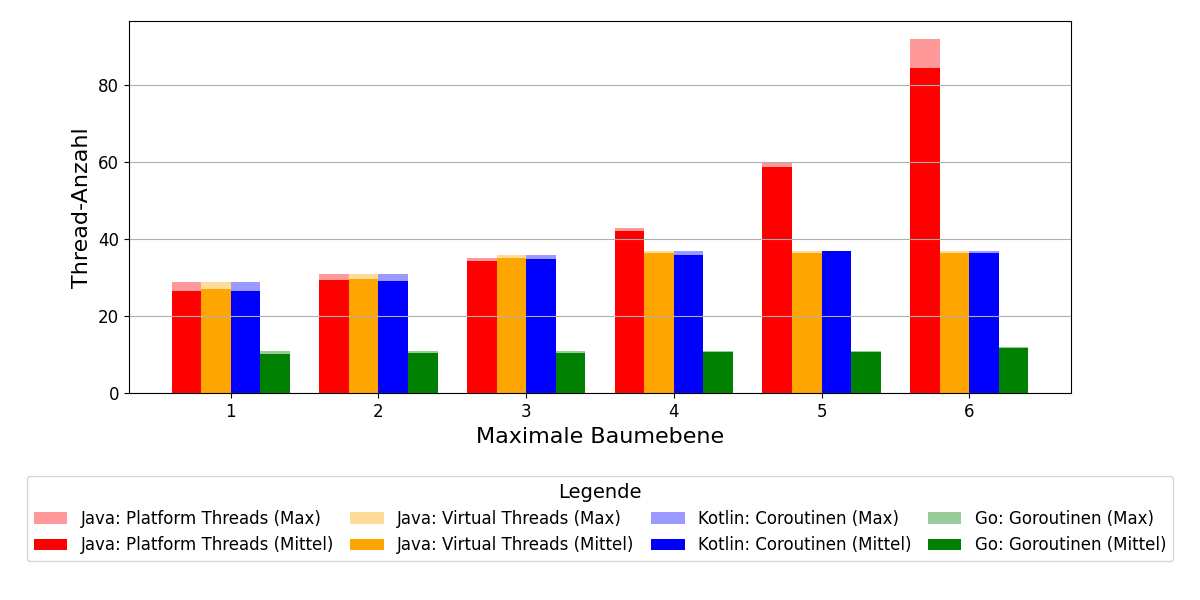
\includegraphics[scale=0.5]{figures/mergesort/Maximalebauebenen1-6/num_threads_bar_plot.png}
	\caption{Mergesort max. Baumebenen:1-6: Thread-Anzahl}
	\label{fig:ms1-6Threads}
\end{figure}

\begin{table}[h]
	\centering
	\small
	\renewcommand{\arraystretch}{1.2} % Erhöhte Zeilenhöhe
	\rowcolors{2}{gray!10}{white} % Alternierende Zeilenfarben ab der zweiten Zeile
	\begin{tabularx}{\textwidth}{XXXXXXXXX} % 9 gleichmäßig verteilte Spalten
		\toprule
		\rowcolor{gray!20} % Kopfzeile farbig
		\textbf{\makecell[l]{Max \\ Baum- \\ ebene}} & 
		\textbf{\makecell[l]{JVT \\ Max \\ Thread}} & 
		\textbf{\makecell[l]{JVT \\ Mittel \\ Thread}} & 
		\textbf{\makecell[l]{JPT \\ Max \\ Thread}} & 
		\textbf{\makecell[l]{JPT \\ Mittel \\ Thread}} & 
		\textbf{\makecell[l]{Coro\\ Max \\ Thread}} & 
		\textbf{\makecell[l]{Coro\\ Mittel \\ Thread}} & 
		\textbf{\makecell[l]{Goro\\ Max \\ Thread}} & 
		\textbf{\makecell[l]{Goro\\ Mittel \\ Thread}} \\
		\midrule
		\csvreader[
		head to column names,
		late after line=\\
		]{measurements/mergesort/Maximalebauebenen1-6/num_threads_aggregated.csv}{}
		{\csvcoli & 
			\pgfmathparse{\csvcolii}\pgfmathprintnumber{\pgfmathresult} & 
			\pgfmathparse{\csvcoliii}\pgfmathprintnumber{\pgfmathresult} & 
			\pgfmathparse{\csvcoliv}\pgfmathprintnumber{\pgfmathresult} & 
			\pgfmathparse{\csvcolv}\pgfmathprintnumber{\pgfmathresult} & 
			\pgfmathparse{\csvcolvi}\pgfmathprintnumber{\pgfmathresult} & 
			\pgfmathparse{\csvcolvii}\pgfmathprintnumber{\pgfmathresult} & 
			\pgfmathparse{\csvcolviii}\pgfmathprintnumber{\pgfmathresult} & 
			\pgfmathparse{\csvcolix}\pgfmathprintnumber{\pgfmathresult}}
		\bottomrule
	\end{tabularx}
	\caption{\textbf{Mergesort max. Baumebenen:1-6: Thread-Anzahl}}
	\label{tab:ms1-6Threads}
\end{table}

\subsubsection{Messung 2: Mergesort - Baumebenen:1-19}

\begin{figure}[H]
	\centering
	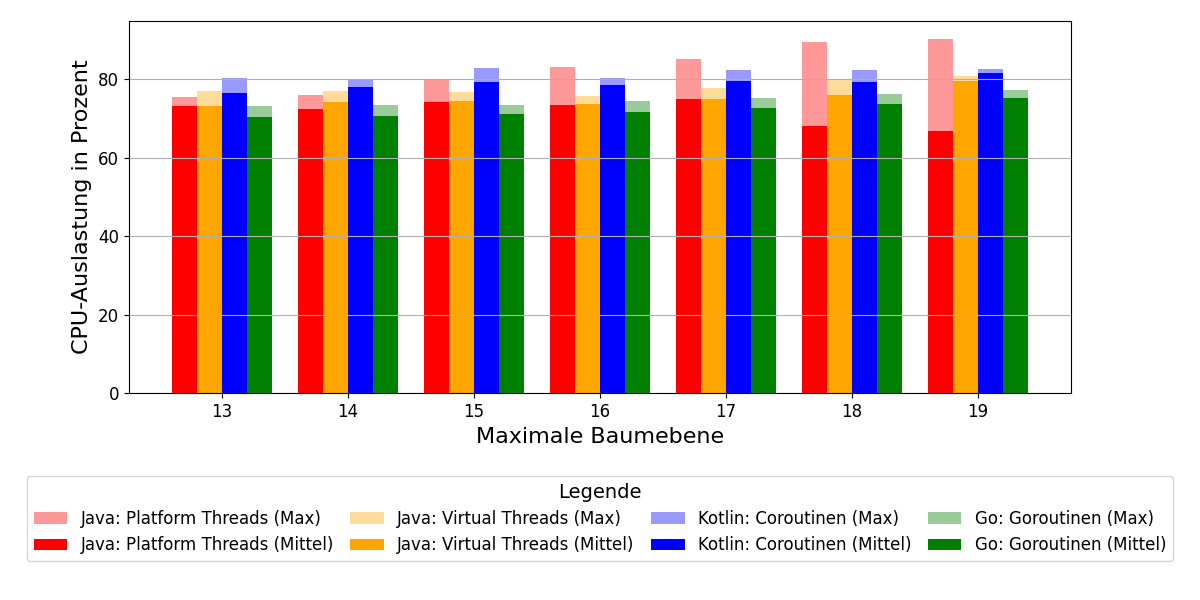
\includegraphics[scale=0.5]{figures/mergesort/Maximalebauebenen1-19_pvcg/cpu_usage_bar_plot.png}
	\caption{Mergesort max. Baumebenen:1-19: CPU-Auslastung}
	\label{fig:ms1-19CPU}
\end{figure}

\begin{table}[H]
	\centering
	\renewcommand{\arraystretch}{1.2} % Erhöhte Zeilenhöhe
	\rowcolors{2}{gray!10}{white} % Alternierende Zeilenfarben ab der zweiten Zeile
	\begin{tabularx}{\textwidth}{XXXXXXXXX} % 9 gleichmäßig verteilte Spalten
		\toprule
		\rowcolor{gray!20} % Kopfzeile farbig
		\textbf{\makecell[l]{Max \\ Baum- \\ ebene}} & 
		\textbf{\makecell[l]{JVT \\ Max \\ CPU}} & 
		\textbf{\makecell[l]{JVT \\ Mittel \\ CPU}} & 
		\textbf{\makecell[l]{JPT \\ Max \\ CPU}} & 
		\textbf{\makecell[l]{JPT \\ Mittel \\ CPU}} & 
		\textbf{\makecell[l]{Coro\\ Max \\ CPU}} & 
		\textbf{\makecell[l]{Coro\\ Mittel \\ CPU}} & 
		\textbf{\makecell[l]{Goro\\ Max \\ CPU}} & 
		\textbf{\makecell[l]{Goro\\ Mittel \\ CPU}} \\
		\midrule
		\csvreader[
		head to column names,
		late after line=\\
		]{measurements/mergesort/Maximalebauebenen1-19_pvcg/cpu_usage_aggregated.csv}{}
		{\csvcoli & 
			\pgfmathparse{\csvcolii}\pgfmathprintnumber{\pgfmathresult}\% & 
			\pgfmathparse{\csvcoliii}\pgfmathprintnumber{\pgfmathresult}\% & 
			\pgfmathparse{\csvcoliv}\pgfmathprintnumber{\pgfmathresult}\% & 
			\pgfmathparse{\csvcolv}\pgfmathprintnumber{\pgfmathresult}\% & 
			\pgfmathparse{\csvcolvi}\pgfmathprintnumber{\pgfmathresult}\% & 
			\pgfmathparse{\csvcolvii}\pgfmathprintnumber{\pgfmathresult}\% & 
			\pgfmathparse{\csvcolviii}\pgfmathprintnumber{\pgfmathresult}\% & 
			\pgfmathparse{\csvcolix}\pgfmathprintnumber{\pgfmathresult}\%}
		\bottomrule
	\end{tabularx}
	\caption{\textbf{Mergesort max. Baumebenen 1-19: CPU-Auslastung}}
	\label{tab:ms1-19CPU}
\end{table}

\begin{figure}[H]
	\centering
	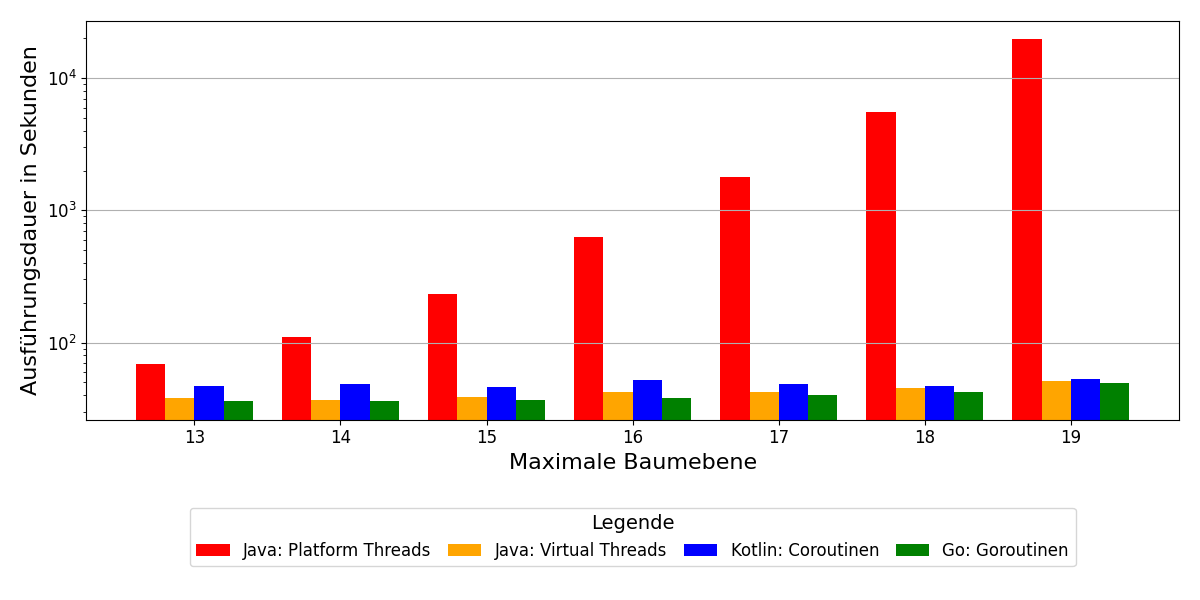
\includegraphics[scale=0.5]{figures/mergesort/Maximalebauebenen1-19_pvcg/execution_time_plot.png}
	\caption{Mergesort max. Baumebenen:1-19: Ausführungszeit}
	\label{fig:ms1-19Zeit}
\end{figure}

\begin{table}[H]
	\centering
	\renewcommand{\arraystretch}{1.2} % Erhöhte Zeilenhöhe
	\rowcolors{2}{gray!10}{white} % Alternierende Zeilenfarben ab der zweiten Zeile
	\begin{tabularx}{\textwidth}{XXXXX} % 9 gleichmäßig verteilte Spalten
		\toprule
		\rowcolor{gray!20} % Kopfzeile farbig
		\textbf{\makecell[l]{Max \\ Baum- \\ ebene}} & 
		\textbf{\makecell[l]{JVT \\ Zeit \\ Gesamt}} & 
		\textbf{\makecell[l]{JPT \\ Zeit \\ Gesamt}} & 
		\textbf{\makecell[l]{Coro\\ Zeit \\ Gesamt}} & 
		\textbf{\makecell[l]{Goro\\ Zeit \\ Gesamt}} \\
		\midrule
		\csvreader[
		head to column names,
		late after line=\\
		]{measurements/mergesort/Maximalebauebenen1-19_pvcg/execution_time_aggregated.csv}{}
		{\csvcoli & 
			\pgfmathparse{\csvcolii}\pgfmathprintnumber{\pgfmathresult} s & 
			\pgfmathparse{\csvcoliii}\pgfmathprintnumber{\pgfmathresult} s & 
			\pgfmathparse{\csvcoliv}\pgfmathprintnumber{\pgfmathresult} s & 
			\pgfmathparse{\csvcolv}\pgfmathprintnumber{\pgfmathresult} s}
		\bottomrule
	\end{tabularx}
	\caption{\textbf{Mergesort max. Baumebenen:1-19: Ausführungszeit}}
	\label{tab:ms1-19Zeit}
\end{table}

\begin{figure}[H]
	\centering
	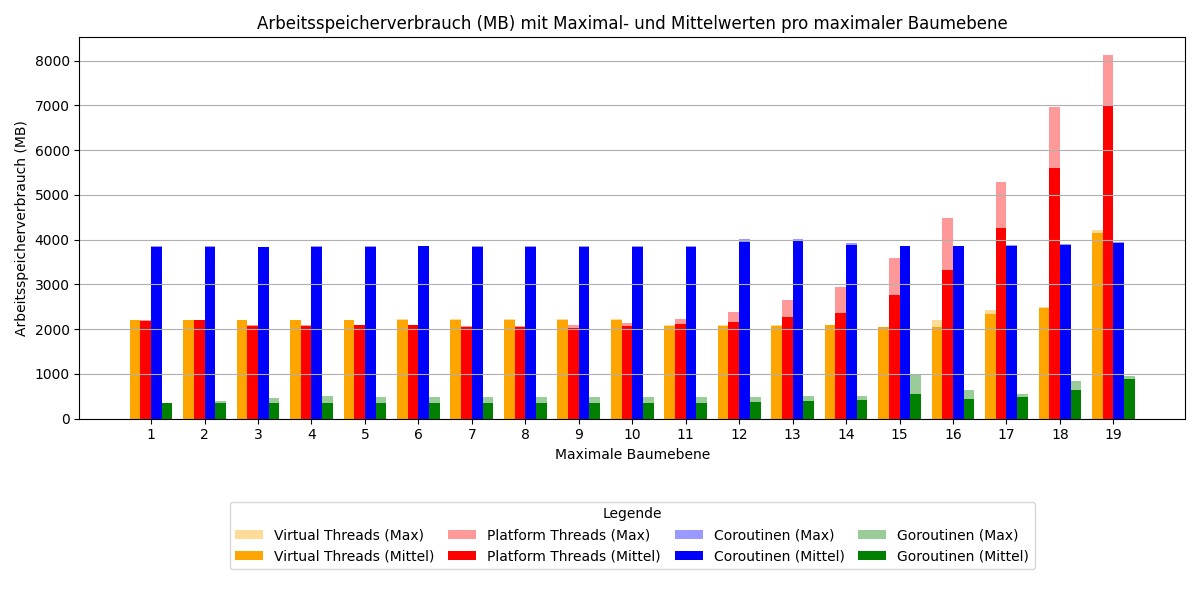
\includegraphics[scale=0.5]{figures/mergesort/Maximalebauebenen1-19_pvcg/memory_usage_bar_plot.png}
	\caption{Mergesort max. Baumebenen:1-19: Arbeitsspeicherverbrauch}
	\label{fig:ms1-19RAM}
\end{figure}

\begin{table}[H]
	\centering
	\renewcommand{\arraystretch}{1.2} % Erhöhte Zeilenhöhe
	\rowcolors{2}{gray!10}{white} % Alternierende Zeilenfarben ab der zweiten Zeile
	\begin{tabularx}{\textwidth}{XXXXXXXXX} % 9 gleichmäßig verteilte Spalten
		\toprule
		\rowcolor{gray!20} % Kopfzeile farbig
		\textbf{\makecell[l]{Max \\ Baum- \\ ebene}} & 
		\textbf{\makecell[l]{JVT \\ Max \\ RAM}} & 
		\textbf{\makecell[l]{JVT \\ Mittel \\ RAM}} & 
		\textbf{\makecell[l]{JPT \\ Max \\ RAM}} & 
		\textbf{\makecell[l]{JPT \\ Mittel \\ RAM}} & 
		\textbf{\makecell[l]{Coro\\ Max \\ RAM}} & 
		\textbf{\makecell[l]{Coro\\ Mittel \\ RAM}} & 
		\textbf{\makecell[l]{Goro\\ Max \\ RAM}} & 
		\textbf{\makecell[l]{Goro\\ Mittel \\ RAM}} \\
		\midrule
		\csvreader[
		head to column names,
		late after line=\\
		]{measurements/mergesort/Maximalebauebenen1-19_pvcg/memory_usage_aggregated.csv}{}
		{\csvcoli & 
			\pgfmathparse{\csvcolii}\pgfmathprintnumber{\pgfmathresult} & 
			\pgfmathparse{\csvcoliii}\pgfmathprintnumber{\pgfmathresult} & 
			\pgfmathparse{\csvcoliv}\pgfmathprintnumber{\pgfmathresult} & 
			\pgfmathparse{\csvcolv}\pgfmathprintnumber{\pgfmathresult} & 
			\pgfmathparse{\csvcolvi}\pgfmathprintnumber{\pgfmathresult} & 
			\pgfmathparse{\csvcolvii}\pgfmathprintnumber{\pgfmathresult} & 
			\pgfmathparse{\csvcolviii}\pgfmathprintnumber{\pgfmathresult} & 
			\pgfmathparse{\csvcolix}\pgfmathprintnumber{\pgfmathresult}}
		\bottomrule
	\end{tabularx}
	\caption{\textbf{Mergesort max. Baumebenen 1-19: Arbeitsspeicherverbrauch}}
	\label{tab:ms1-19RAM}
	\vspace{-10mm}  % optional: Anpassung des Abstands zur Tabelle
	\textit{Einheit: MB}
\end{table}

\begin{figure}[H]
	\centering
	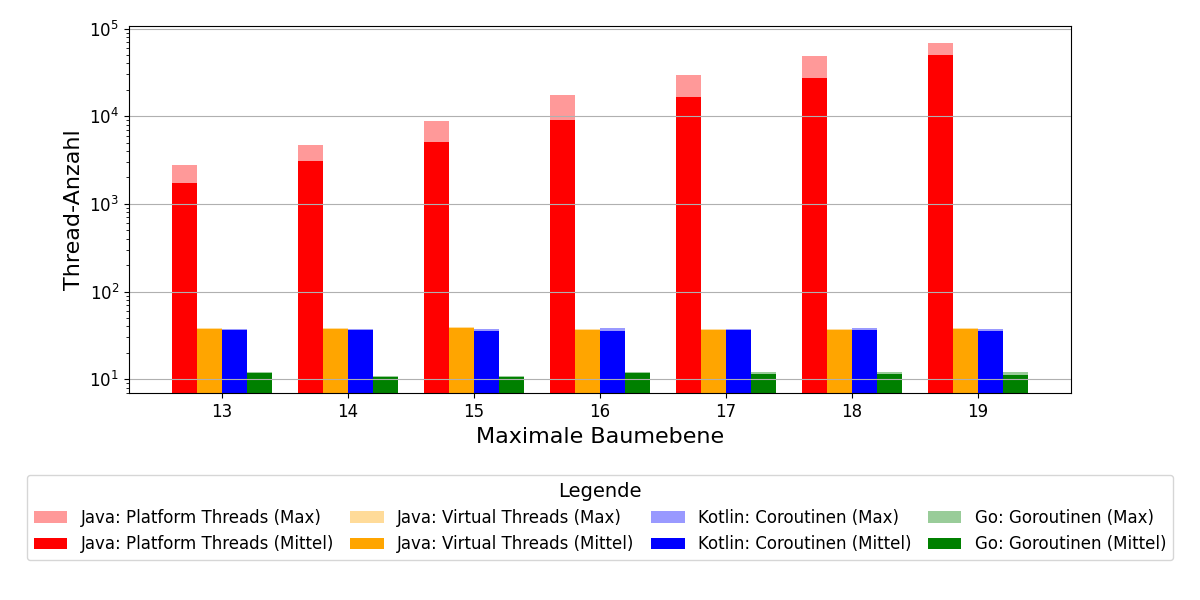
\includegraphics[scale=0.5]{figures/mergesort/Maximalebauebenen1-19_pvcg/num_threads_bar_plot.png}
	\caption{Mergesort max. Baumebenen:1-19: Thread-Anzahl}
	\label{fig:ms1-19Threads}
\end{figure}

\begin{table}[H]
	\centering
	\small
	\renewcommand{\arraystretch}{1.2} % Erhöhte Zeilenhöhe
	\rowcolors{2}{gray!10}{white} % Alternierende Zeilenfarben ab der zweiten Zeile
	\begin{tabularx}{\textwidth}{XXXXXXXXX} % 9 gleichmäßig verteilte Spalten
		\toprule
		\rowcolor{gray!20} % Kopfzeile farbig
		\textbf{\makecell[l]{Max \\ Baum- \\ ebene}} & 
		\textbf{\makecell[l]{JVT \\ Max \\ Thread}} & 
		\textbf{\makecell[l]{JVT \\ Mittel \\ Thread}} & 
		\textbf{\makecell[l]{JPT \\ Max \\ Thread}} & 
		\textbf{\makecell[l]{JPT \\ Mittel \\ Thread}} & 
		\textbf{\makecell[l]{Coro\\ Max \\ Thread}} & 
		\textbf{\makecell[l]{Coro\\ Mittel \\ Thread}} & 
		\textbf{\makecell[l]{Goro\\ Max \\ Thread}} & 
		\textbf{\makecell[l]{Goro\\ Mittel \\ Thread}} \\
		\midrule
		\csvreader[
		head to column names,
		late after line=\\
		]{measurements/mergesort/Maximalebauebenen1-19_pvcg/num_threads_aggregated.csv}{}
		{\csvcoli & 
			\pgfmathparse{\csvcolii}\pgfmathprintnumber{\pgfmathresult} & 
			\pgfmathparse{\csvcoliii}\pgfmathprintnumber{\pgfmathresult} & 
			\pgfmathparse{\csvcoliv}\pgfmathprintnumber{\pgfmathresult} & 
			\pgfmathparse{\csvcolv}\pgfmathprintnumber{\pgfmathresult} & 
			\pgfmathparse{\csvcolvi}\pgfmathprintnumber{\pgfmathresult} & 
			\pgfmathparse{\csvcolvii}\pgfmathprintnumber{\pgfmathresult} & 
			\pgfmathparse{\csvcolviii}\pgfmathprintnumber{\pgfmathresult} & 
			\pgfmathparse{\csvcolix}\pgfmathprintnumber{\pgfmathresult}}
		\bottomrule
	\end{tabularx}
	\caption{\textbf{Mergesort max. Baumebenen:1-19: Thread-Anzahl}}
	\label{tab:ms1-19Threads}
\end{table}

\subsubsection{Messung 3: Mergesort - Baumebenen:1-23}

ohne Platform Threads!!!

\begin{figure}[H]
	\centering
	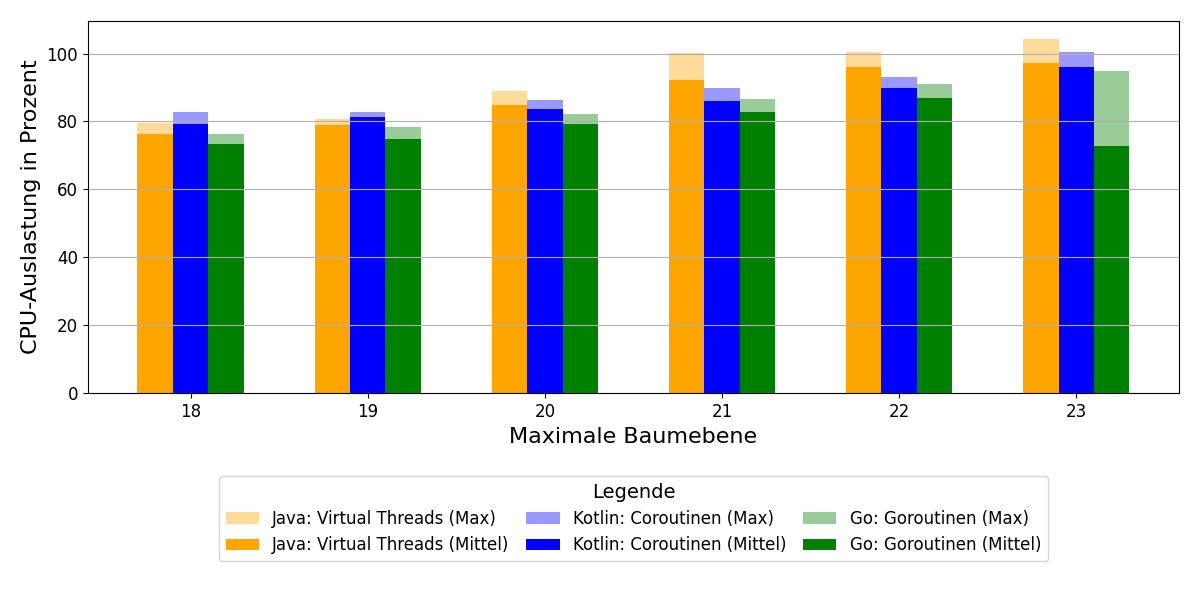
\includegraphics[scale=0.5]{figures/mergesort/Maximalebauebenen1-23_vcg/cpu_usage_bar_plot.png}
	\caption{Mergesort max. Baumebenen:1-23: CPU-Auslastung}
	\label{fig:ms1-23CPU}
\end{figure}

\begin{table}[H]
	\centering
	\renewcommand{\arraystretch}{1.2} % Erhöhte Zeilenhöhe
	\rowcolors{2}{gray!10}{white} % Alternierende Zeilenfarben ab der zweiten Zeile
	\begin{tabularx}{\textwidth}{XXXXXXX} % 7 gleichmäßig verteilte Spalten
		\toprule
		\rowcolor{gray!20} % Kopfzeile farbig
		\textbf{\makecell[l]{Max \\ Baum- \\ ebene}} & 
		\textbf{\makecell[l]{JVT \\ Max \\ CPU}} & 
		\textbf{\makecell[l]{JVT \\ Mittel \\ CPU}} &
		\textbf{\makecell[l]{Coro\\ Max \\ CPU}} & 
		\textbf{\makecell[l]{Coro\\ Mittel \\ CPU}} & 
		\textbf{\makecell[l]{Goro\\ Max \\ CPU}} & 
		\textbf{\makecell[l]{Goro\\ Mittel \\ CPU}} \\
		\midrule
		\csvreader[
		head to column names,
		late after line=\\
		]{measurements/mergesort/Maximalebauebenen1-23_vcg/cpu_usage_aggregated.csv}{}
		{\csvcoli & 
			\pgfmathparse{\csvcolii}\pgfmathprintnumber{\pgfmathresult}\% & 
			\pgfmathparse{\csvcoliii}\pgfmathprintnumber{\pgfmathresult}\% & 
			\pgfmathparse{\csvcoliv}\pgfmathprintnumber{\pgfmathresult}\% & 
			\pgfmathparse{\csvcolv}\pgfmathprintnumber{\pgfmathresult}\% & 
			\pgfmathparse{\csvcolvi}\pgfmathprintnumber{\pgfmathresult}\% & 
			\pgfmathparse{\csvcolvii}\pgfmathprintnumber{\pgfmathresult}\%}
		\bottomrule
	\end{tabularx}
	\caption{\textbf{Mergesort max. Baumebenen 1-23: CPU-Auslastung}}
	\label{tab:ms1-23CPU}
\end{table}

\begin{figure}[H]
	\centering
	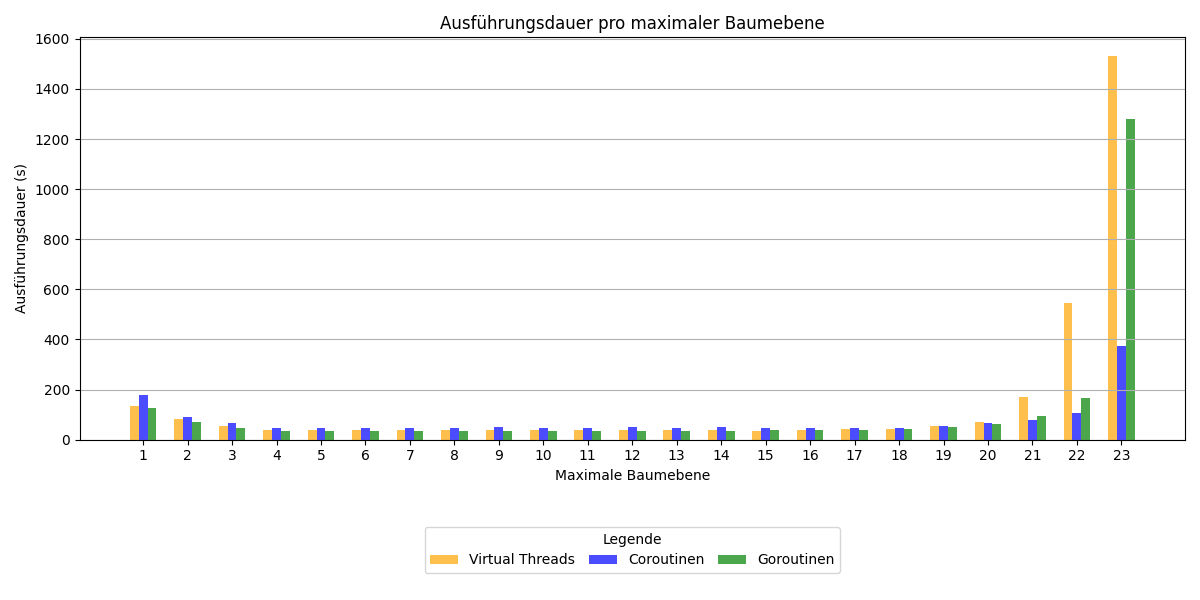
\includegraphics[scale=0.5]{figures/mergesort/Maximalebauebenen1-23_vcg/execution_time_plot.png}
	\caption{Mergesort max. Baumebenen:1-23: Ausführungszeit}
	\label{fig:ms1-23Zeit}
\end{figure}

\begin{table}[H]
	\centering
	\renewcommand{\arraystretch}{1.2} % Erhöhte Zeilenhöhe
	\rowcolors{2}{gray!10}{white} % Alternierende Zeilenfarben ab der zweiten Zeile
	\begin{tabularx}{\textwidth}{XXXX} % 9 gleichmäßig verteilte Spalten
		\toprule
		\rowcolor{gray!20} % Kopfzeile farbig
		\textbf{\makecell[l]{Max \\ Baum- \\ ebene}} & 
		\textbf{\makecell[l]{JVT \\ Zeit \\ Gesamt}} & 
		\textbf{\makecell[l]{Coro\\ Zeit \\ Gesamt}} & 
		\textbf{\makecell[l]{Goro\\ Zeit \\ Gesamt}} \\
		\midrule
		\csvreader[
		head to column names,
		late after line=\\
		]{measurements/mergesort/Maximalebauebenen1-23_vcg/execution_time_aggregated.csv}{}
		{\csvcoli & 
			\pgfmathparse{\csvcolii}\pgfmathprintnumber{\pgfmathresult} s & 
			\pgfmathparse{\csvcoliii}\pgfmathprintnumber{\pgfmathresult} s & 
			\pgfmathparse{\csvcoliv}\pgfmathprintnumber{\pgfmathresult} s}
		\bottomrule
	\end{tabularx}
	\caption{\textbf{Mergesort max. Baumebenen:1-23: Ausführungszeit}}
	\label{tab:ms1-23Zeit}
\end{table}

\begin{figure}[H]
	\centering
	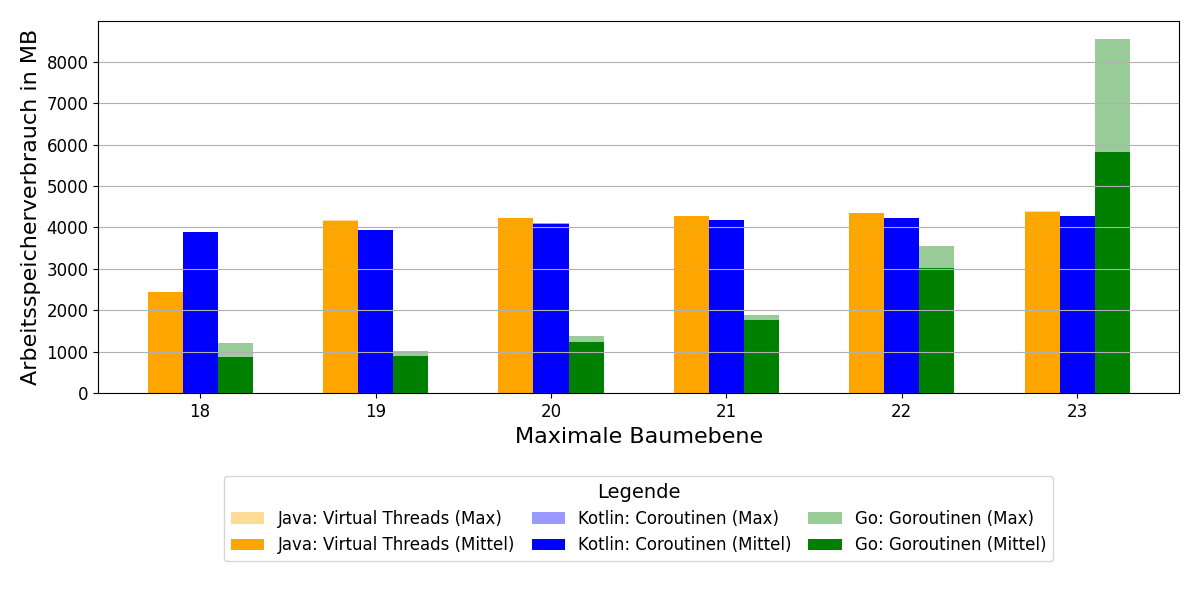
\includegraphics[scale=0.5]{figures/mergesort/Maximalebauebenen1-23_vcg/memory_usage_bar_plot.png}
	\caption{Mergesort max. Baumebenen:1-23: Arbeitsspeicherverbrauch}
	\label{fig:ms1-23RAM}
\end{figure}

\begin{table}[H]
	\centering
	\renewcommand{\arraystretch}{1.2} % Erhöhte Zeilenhöhe
	\rowcolors{2}{gray!10}{white} % Alternierende Zeilenfarben ab der zweiten Zeile
	\begin{tabularx}{\textwidth}{XXXXXXX} % 9 gleichmäßig verteilte Spalten
		\toprule
		\rowcolor{gray!20} % Kopfzeile farbig
		\textbf{\makecell[l]{Max \\ Baum- \\ ebene}} & 
		\textbf{\makecell[l]{JVT \\ Max \\ RAM}} & 
		\textbf{\makecell[l]{JVT \\ Mittel \\ RAM}} & 
		\textbf{\makecell[l]{Coro\\ Max \\ RAM}} & 
		\textbf{\makecell[l]{Coro\\ Mittel \\ RAM}} & 
		\textbf{\makecell[l]{Goro\\ Max \\ RAM}} & 
		\textbf{\makecell[l]{Goro\\ Mittel \\ RAM}} \\
		\midrule
		\csvreader[
		head to column names,
		late after line=\\
		]{measurements/mergesort/Maximalebauebenen1-23_vcg/memory_usage_aggregated.csv}{}
		{\csvcoli & 
			\pgfmathparse{\csvcolii}\pgfmathprintnumber{\pgfmathresult} & 
			\pgfmathparse{\csvcoliii}\pgfmathprintnumber{\pgfmathresult} & 
			\pgfmathparse{\csvcoliv}\pgfmathprintnumber{\pgfmathresult} & 
			\pgfmathparse{\csvcolv}\pgfmathprintnumber{\pgfmathresult} & 
			\pgfmathparse{\csvcolvi}\pgfmathprintnumber{\pgfmathresult} & 
			\pgfmathparse{\csvcolvii}\pgfmathprintnumber{\pgfmathresult}}
		\bottomrule
	\end{tabularx}
	\caption{\textbf{Mergesort max. Baumebenen 1-23: Arbeitsspeicherverbrauch}}
	\label{tab:ms1-23RAM}
	\vspace{-10mm}  % optional: Anpassung des Abstands zur Tabelle
	\textit{Einheit: MB}
\end{table}

\begin{figure}[H]
	\centering
	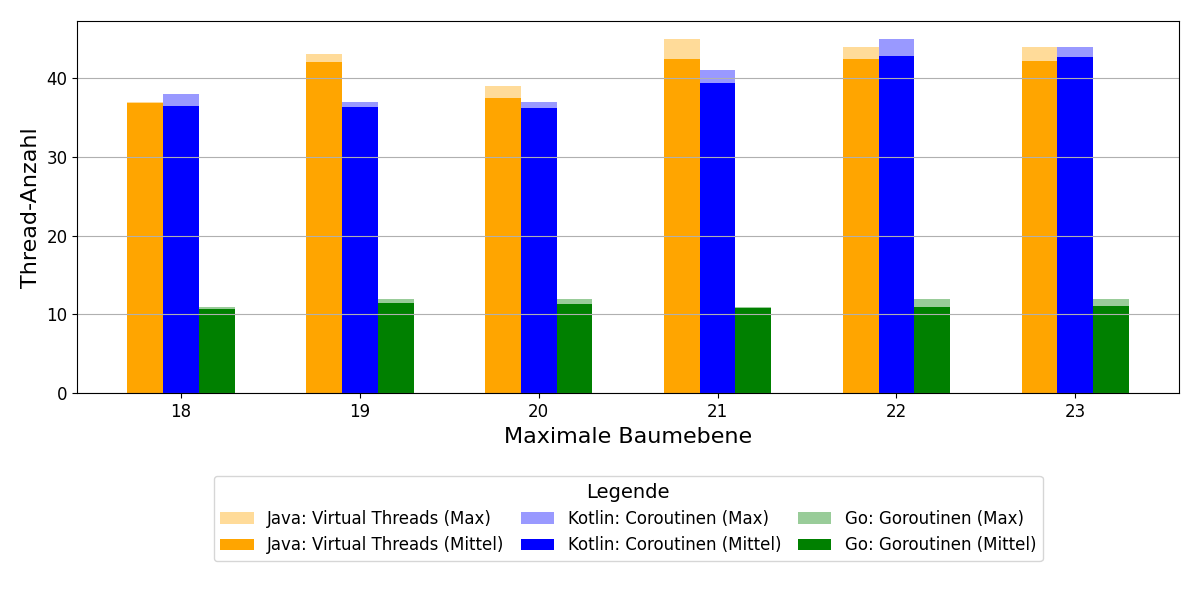
\includegraphics[scale=0.5]{figures/mergesort/Maximalebauebenen1-23_vcg/num_threads_bar_plot.png}
	\caption{Mergesort max. Baumebenen:1-23: Thread-Anzahl}
	\label{fig:ms1-23Threads}
\end{figure}

\begin{table}[H]
	\centering
	\small
	\renewcommand{\arraystretch}{1.2} % Erhöhte Zeilenhöhe
	\rowcolors{2}{gray!10}{white} % Alternierende Zeilenfarben ab der zweiten Zeile
	\begin{tabularx}{\textwidth}{XXXXXXX} % 9 gleichmäßig verteilte Spalten
		\toprule
		\rowcolor{gray!20} % Kopfzeile farbig
		\textbf{\makecell[l]{Max \\ Baum- \\ ebene}} & 
		\textbf{\makecell[l]{JVT \\ Max \\ Thread}} & 
		\textbf{\makecell[l]{JVT \\ Mittel \\ Thread}} & 
		\textbf{\makecell[l]{Coro\\ Max \\ Thread}} & 
		\textbf{\makecell[l]{Coro\\ Mittel \\ Thread}} & 
		\textbf{\makecell[l]{Goro\\ Max \\ Thread}} & 
		\textbf{\makecell[l]{Goro\\ Mittel \\ Thread}} \\
		\midrule
		\csvreader[
		head to column names,
		late after line=\\
		]{measurements/mergesort/Maximalebauebenen1-23_vcg/num_threads_aggregated.csv}{}
		{\csvcoli & 
			\pgfmathparse{\csvcolii}\pgfmathprintnumber{\pgfmathresult} & 
			\pgfmathparse{\csvcoliii}\pgfmathprintnumber{\pgfmathresult} & 
			\pgfmathparse{\csvcoliv}\pgfmathprintnumber{\pgfmathresult} & 
			\pgfmathparse{\csvcolv}\pgfmathprintnumber{\pgfmathresult} & 
			\pgfmathparse{\csvcolvi}\pgfmathprintnumber{\pgfmathresult} & 
			\pgfmathparse{\csvcolvii}\pgfmathprintnumber{\pgfmathresult}}
		\bottomrule
	\end{tabularx}
	\caption{\textbf{Mergesort max. Baumebenen:1-23: Thread-Anzahl}}
	\label{tab:ms1-23Threads}
\end{table}

\subsubsection{Messung 4: Mergesort - Listenlänge}

Faktor 10!!!

\begin{figure}[H]
	\centering
	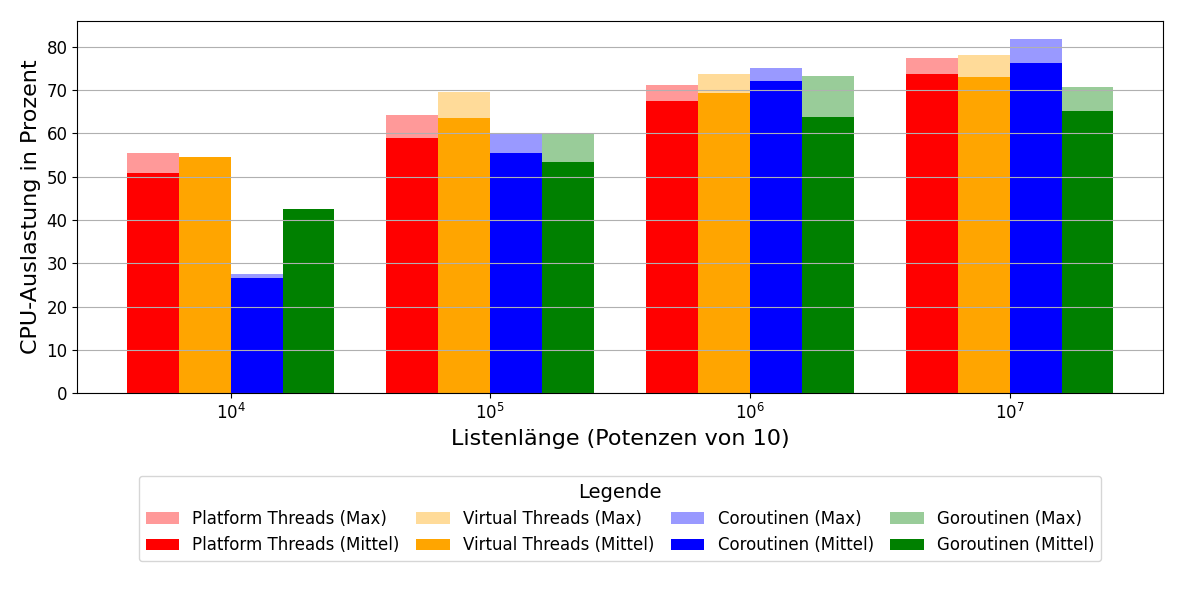
\includegraphics[scale=0.5]{figures/mergesort/Listenlaenge/cpu_usage_bar_plot.png}
	\caption{Mergesort Listenlänge: CPU-Auslastung}
	\label{fig:mslaengeCPU}
\end{figure}

\begin{table}[H]
	\centering
	\renewcommand{\arraystretch}{1.2} % Erhöhte Zeilenhöhe
	\rowcolors{2}{gray!10}{white} % Alternierende Zeilenfarben ab der zweiten Zeile
	\begin{tabularx}{\textwidth}{>{\hsize=4\hsize}X*{8}{>{\hsize=3.11\hsize}X}}
		\toprule
		\rowcolor{gray!20} % Kopfzeile farbig
		\textbf{\makecell[l]{Listen- \\ länge}} & 
		\textbf{\makecell[l]{JVT \\ Max \\ CPU}} & 
		\textbf{\makecell[l]{JVT \\ Mittel \\ CPU}} & 
		\textbf{\makecell[l]{JPT \\ Max \\ CPU}} & 
		\textbf{\makecell[l]{JPT \\ Mittel \\ CPU}} & 
		\textbf{\makecell[l]{Coro\\ Max \\ CPU}} & 
		\textbf{\makecell[l]{Coro\\ Mittel \\ CPU}} & 
		\textbf{\makecell[l]{Goro\\ Max \\ CPU}} & 
		\textbf{\makecell[l]{Goro\\ Mittel \\ CPU}} \\
		\midrule
		\csvreader[
		head to column names,
		late after line=\\
		]{measurements/mergesort/Listenlaenge/cpu_usage_aggregated.csv}{}
		{\csvcoli & 
			\pgfmathparse{\csvcolii}\pgfmathprintnumber{\pgfmathresult}\% & 
			\pgfmathparse{\csvcoliii}\pgfmathprintnumber{\pgfmathresult}\% & 
			\pgfmathparse{\csvcoliv}\pgfmathprintnumber{\pgfmathresult}\% & 
			\pgfmathparse{\csvcolv}\pgfmathprintnumber{\pgfmathresult}\% & 
			\pgfmathparse{\csvcolvi}\pgfmathprintnumber{\pgfmathresult}\% & 
			\pgfmathparse{\csvcolvii}\pgfmathprintnumber{\pgfmathresult}\% & 
			\pgfmathparse{\csvcolviii}\pgfmathprintnumber{\pgfmathresult}\% & 
			\pgfmathparse{\csvcolix}\pgfmathprintnumber{\pgfmathresult}\%}
		\bottomrule
	\end{tabularx}
	\caption{\textbf{Mergesort Listenlänge: CPU-Auslastung}}
	\label{tab:mslaengeCPU}
\end{table}

\begin{figure}[H]
	\centering
	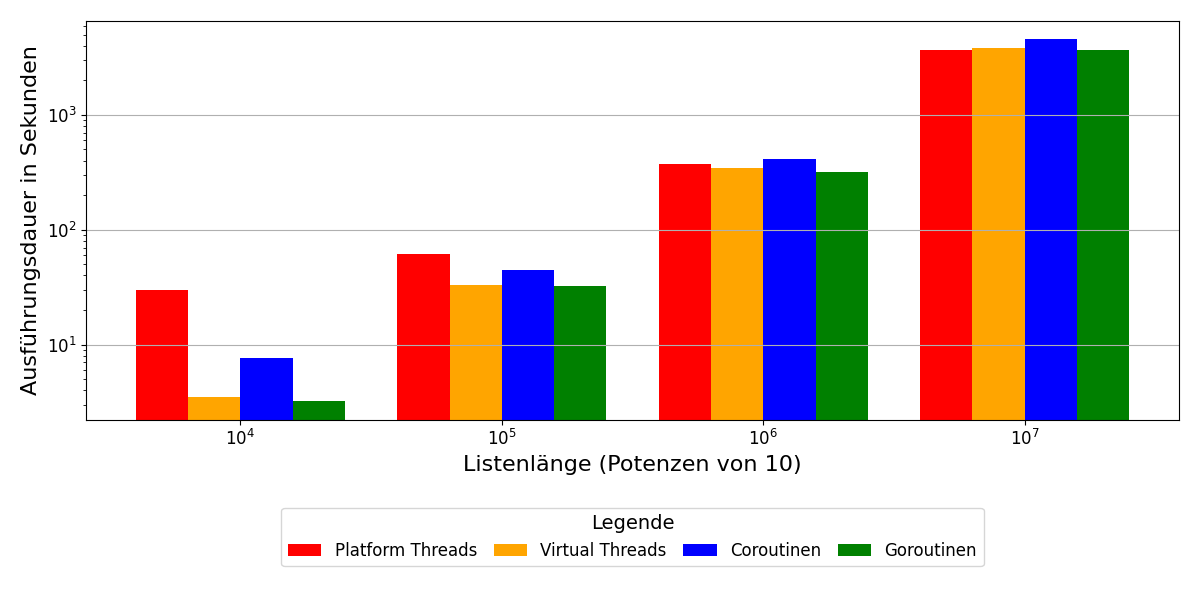
\includegraphics[scale=0.5]{figures/mergesort/Listenlaenge/execution_time_plot.png}
	\caption{Mergesort Listenlänge: Ausführungszeit}
	\label{fig:mslaengeZeit}
\end{figure}

\begin{table}[H]
	\centering
	\renewcommand{\arraystretch}{1.2} % Erhöhte Zeilenhöhe
	\rowcolors{2}{gray!10}{white} % Alternierende Zeilenfarben ab der zweiten Zeile
	\begin{tabularx}{\textwidth}{XXXXX} % 5 gleichmäßig verteilte Spalten
		\toprule
		\rowcolor{gray!20} % Kopfzeile farbig
		\textbf{\makecell[l]{Listen- \\ länge}} & 
		\textbf{\makecell[l]{JVT \\ Zeit \\ Gesamt}} & 
		\textbf{\makecell[l]{JPT \\ Zeit \\ Gesamt}} & 
		\textbf{\makecell[l]{Coro \\ Zeit \\ Gesamt}} &
		\textbf{\makecell[l]{Goro \\ Zeit \\ Gesamt}} \\
		\midrule
		\csvreader[
		head to column names,
		late after line=\\
		]{measurements/mergesort/Listenlaenge/execution_time_aggregated.csv}{}
		{\csvcoli & 
			\pgfmathparse{\csvcolii}\pgfmathprintnumber{\pgfmathresult} s & 
			\pgfmathparse{\csvcoliii}\pgfmathprintnumber{\pgfmathresult} s & 
			\pgfmathparse{\csvcoliv}\pgfmathprintnumber{\pgfmathresult} s & 
			\pgfmathparse{\csvcolv}\pgfmathprintnumber{\pgfmathresult} s}
		\bottomrule
	\end{tabularx}
	\caption{\textbf{Mergesort Listenlänge: Ausführungszeit}}
	\label{tab:mslaengeZeit}
\end{table}

\begin{figure}[H]
	\centering
	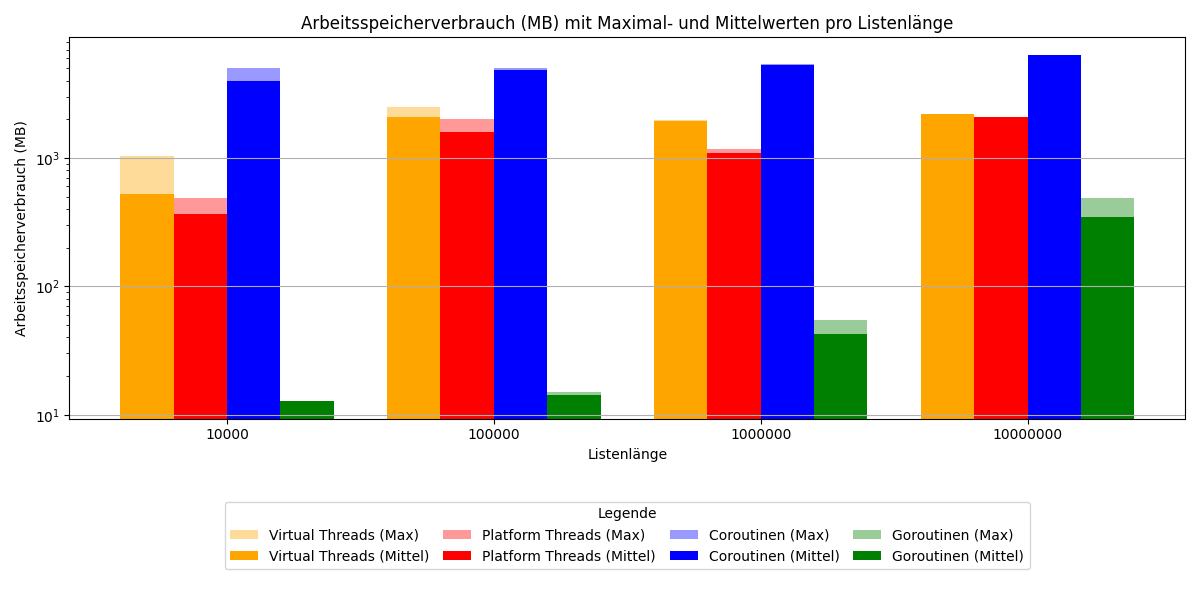
\includegraphics[scale=0.5]{figures/mergesort/Listenlaenge/memory_usage_bar_plot.png}
	\caption{Mergesort Listenlänge: Arbeitsspeicherverbrauch}
	\label{fig:mslaengeRAM}
\end{figure}

\begin{table}[H]
	\centering
	\renewcommand{\arraystretch}{1.2} % Erhöhte Zeilenhöhe
	\rowcolors{2}{gray!10}{white} % Alternierende Zeilenfarben ab der zweiten Zeile
	\begin{tabularx}{\textwidth}{>{\hsize=4\hsize}X*{8}{>{\hsize=3.11\hsize}X}}
		\toprule
		\rowcolor{gray!20} % Kopfzeile farbig
		\textbf{\makecell[l]{Listen- \\ länge}} & 
		\textbf{\makecell[l]{JVT \\ Max \\ RAM}} & 
		\textbf{\makecell[l]{JVT \\ Mittel \\ RAM}} & 
		\textbf{\makecell[l]{JPT \\ Max \\ RAM}} & 
		\textbf{\makecell[l]{JPT \\ Mittel \\ RAM}} & 
		\textbf{\makecell[l]{Coro\\ Max \\ RAM}} & 
		\textbf{\makecell[l]{Coro\\ Mittel \\ RAM}} & 
		\textbf{\makecell[l]{Goro\\ Max \\ RAM}} & 
		\textbf{\makecell[l]{Goro\\ Mittel \\ RAM}} \\
		\midrule
		\csvreader[
		head to column names,
		late after line=\\
		]{measurements/mergesort/Listenlaenge/memory_usage_aggregated.csv}{}
		{\csvcoli & 
			\pgfmathparse{\csvcolii}\pgfmathprintnumber{\pgfmathresult} & 
			\pgfmathparse{\csvcoliii}\pgfmathprintnumber{\pgfmathresult} & 
			\pgfmathparse{\csvcoliv}\pgfmathprintnumber{\pgfmathresult} & 
			\pgfmathparse{\csvcolv}\pgfmathprintnumber{\pgfmathresult} & 
			\pgfmathparse{\csvcolvi}\pgfmathprintnumber{\pgfmathresult} & 
			\pgfmathparse{\csvcolvii}\pgfmathprintnumber{\pgfmathresult} & 
			\pgfmathparse{\csvcolviii}\pgfmathprintnumber{\pgfmathresult} & 
			\pgfmathparse{\csvcolix}\pgfmathprintnumber{\pgfmathresult}}
		\bottomrule
	\end{tabularx}
	\caption{\textbf{Mergesort Listenlänge: Arbeitsspeicherverbrauch}}
	\label{tab:mslaengeRAM}
	\vspace{-10mm}  % optional: Anpassung des Abstands zur Tabelle
	\textit{Einheit: MB}
\end{table}

\begin{figure}[H]
	\centering
	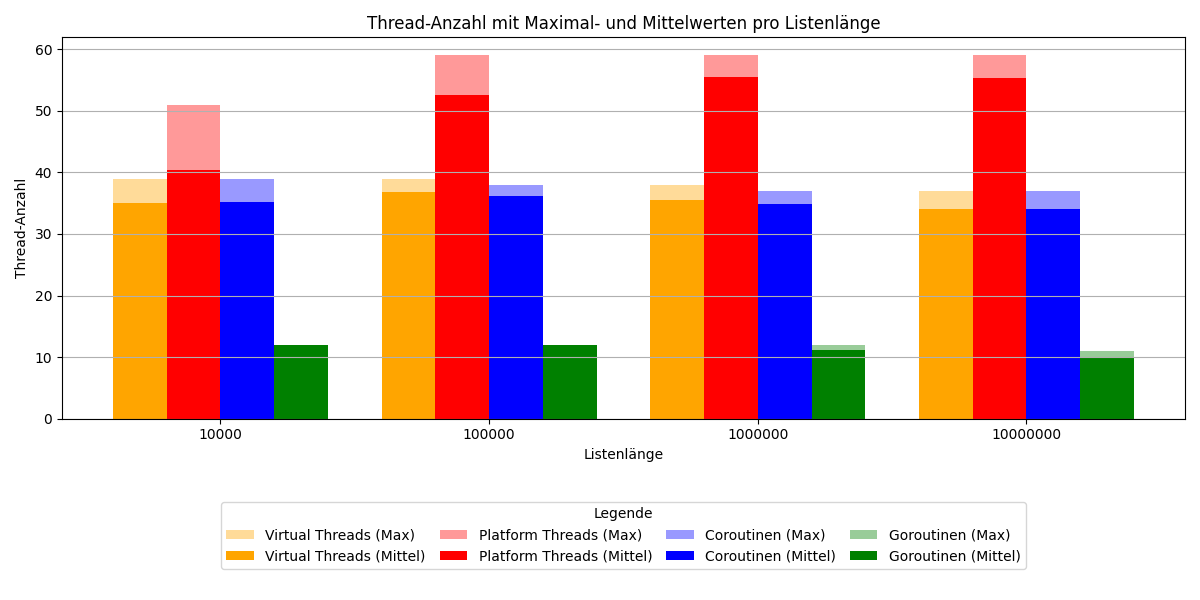
\includegraphics[scale=0.5]{figures/mergesort/Listenlaenge/num_threads_bar_plot.png}
	\caption{Mergesort Listenlänge: Thread-Anzahl}
	\label{fig:mslaengeThreads}
\end{figure}

\begin{table}[H]
	\centering
	\small
	\renewcommand{\arraystretch}{1.2} % Erhöhte Zeilenhöhe
	\rowcolors{2}{gray!10}{white} % Alternierende Zeilenfarben ab der zweiten Zeile
	\begin{tabularx}{\textwidth}{>{\hsize=4\hsize}X*{8}{>{\hsize=3.34\hsize}X}}
		\toprule
		\rowcolor{gray!20} % Kopfzeile farbig
		\textbf{\makecell[l]{Liste- \\ länge}} & 
		\textbf{\makecell[l]{JVT \\ Max \\ Thread}} & 
		\textbf{\makecell[l]{JVT \\ Mittel \\ Thread}} & 
		\textbf{\makecell[l]{JPT \\ Max \\ Thread}} & 
		\textbf{\makecell[l]{JPT \\ Mittel \\ Thread}} & 
		\textbf{\makecell[l]{Coro\\ Max \\ Thread}} & 
		\textbf{\makecell[l]{Coro\\ Mittel \\ Thread}} & 
		\textbf{\makecell[l]{Goro\\ Max \\ Thread}} & 
		\textbf{\makecell[l]{Goro\\ Mittel \\ Thread}} \\
		\midrule
		\csvreader[
		head to column names,
		late after line=\\
		]{measurements/mergesort/Listenlaenge/num_threads_aggregated.csv}{}
		{\csvcoli & 
			\pgfmathparse{\csvcolii}\pgfmathprintnumber{\pgfmathresult} & 
			\pgfmathparse{\csvcoliii}\pgfmathprintnumber{\pgfmathresult} & 
			\pgfmathparse{\csvcoliv}\pgfmathprintnumber{\pgfmathresult} & 
			\pgfmathparse{\csvcolv}\pgfmathprintnumber{\pgfmathresult} & 
			\pgfmathparse{\csvcolvi}\pgfmathprintnumber{\pgfmathresult} & 
			\pgfmathparse{\csvcolvii}\pgfmathprintnumber{\pgfmathresult} & 
			\pgfmathparse{\csvcolviii}\pgfmathprintnumber{\pgfmathresult} & 
			\pgfmathparse{\csvcolix}\pgfmathprintnumber{\pgfmathresult}}
		\bottomrule
	\end{tabularx}
	\caption{\textbf{Mergesort Listenlänge: Thread-Anzahl}}
	\label{tab:mslaengeThreads}
\end{table}

\section{Benchmark 2}

\subsection{Beschreibung: Benchmark 2}

PostgreSQL bietet ein robustes Transaktionskonzept, das die ACID-Eigenschaften (Atomicity, Consistency, Isolation, Durability) gewährleistet.

Eine Transaktion in PostgreSQL ist eine Sequenz von Datenbankoperationen, die als eine einzige, unteilbare Einheit behandelt wird1. Sie beginnt mit dem Befehl BEGIN und endet entweder mit COMMIT, um die Änderungen zu speichern, oder mit ROLLBACK, um sie rückgängig zu machen

PL/pgSQL-Funktionen laufen bereits in einem Transaktionskontext, daher ist die explizite Transaktionskontrolle innerhalb der Funktion nicht erforderlich

Die Fehlerbehandlung mit EXCEPTION ist korrekt implementiert. Sie fängt alle Fehler ab und führt ein ROLLBACK durch, bevor der Fehler weitergegeben wird. Dies ist eine gute Praxis zur Sicherstellung der Datenintegrität.,

Bei der Verwendung von PostgREST sollten Sie beachten, dass es automatisch Transaktionen für jede HTTP-Anfrage verwaltet. Ihre Funktion wird also in diesem Kontext korrekt funktionieren, ohne dass Sie sich um die explizite Transaktionskontrolle kümmern müssen.

Sperren und Wartezeiten:
PostgreSQL verwendet Zeilensperren, um konkurrierende Zugriffe zu verwalten. Wenn eine andere Transaktion bereits Sperren auf den betroffenen Konten hält, wird Ihre transfer\_balance Funktion warten, bis diese Sperren freigegeben werden

Deadlock-Erkennung:
Wenn zwei Transaktionen gegenseitig aufeinander warten, erkennt PostgreSQL den Deadlock und bricht eine der Transaktionen ab


\chapter{Auswertung}

\section{Ergebnisse und Beobachtungen}

\section{Diskussion und Bewertung}



\chapter{Zusammenfassung und Ausblick}

\section{Zusammenfassung}

\section{Ausblick}
%Java VT kein pinning bei Synchronized
%Structured Concurrency(jeps/preview)
%Scoped Values(jeps/preview)



\printbibliography


%\input{abkuerz.tex}      % Einbinden von Tex-Files
%\input{einfuehrung.tex}
%
%\include{normen}        % Einbinden von größeren Tex-Files,z.B. Kapiteln
%\include{aufbau}
%\include{zitieren}
%\include{form}
%\include{allgtips}
%
%\bibliographystyle{alpha}  % Schlüssel als Buchstaben
%\bibliography{literaturverzeichnis}      % Literaturverzeichnis

\end{document}


